

%----------
% DOCUMENT CONFIGURATION
%----------

\documentclass[12pt]{report} %font 12pt

% MARGINS
\usepackage[
a4paper,
vmargin=2.5cm,
hmargin=3cm
]{geometry}

\renewcommand{\baselinestretch}{1.15}
\parskip=6pt

\usepackage{pdflscape}

% COLORS for cover and code
\usepackage[table]{xcolor}
\definecolor{azulUC3M}{RGB}{0,0,102}
\definecolor{gray97}{gray}{.97}
\definecolor{gray75}{gray}{.75}
\definecolor{gray45}{gray}{.45}

% Soporte para GENERAR PDF/A --es importante de cara a su inclusión en e-Archivo porque es el formato óptimo de preservación y a la generación de metadatos, tal y como se describe en http://uc3m.libguides.com/ld.php?content_id=31389625. En la carpeta incluímos el archivo plantilla_tfg_2017.xmpdata en el que puedes incluir los metadatos que se incorporarán al archivo PDF cuando lo compiles. Ese archivo debe llamarse igual que tu archivo .tex. Puedes ver un ejemplo en esta misma carpeta.
\usepackage[a-1b]{pdfx}

% LINKS
\usepackage{hyperref}
\hypersetup{colorlinks=true,
	linkcolor=black,
	urlcolor=blue}

% MATH
\usepackage{amsmath,amssymb,amsfonts,amsthm}

\usepackage{txfonts} 
\usepackage[T1]{fontenc}
\usepackage[utf8]{inputenc}

\usepackage[english]{babel} 
\usepackage[babel, english=american]{csquotes}
\AtBeginEnvironment{quote}{\small}

\usepackage{fancyhdr}
\usepackage{tikz}

% FOOTER
\fancypagestyle{fancy}{
\fancyhf{}
\renewcommand{\headrulewidth}{1pt}
\fancyhead{}         
\fancyhead[LO]{CHAPTER \thechapter}     
\fancyhead[RO]{\rightmark}  
\rfoot{\thepage}
}

\fancypagestyle{plain}{
	%\fancyhf{}
	\pagestyle{plainnofancy}
	%\renewcommand{\headrulewidth}{0pt}
}

\fancypagestyle{plainnofancy}%
{%
\fancyhf{}
\renewcommand{\headrulewidth}{0pt}
\rfoot{\thepage}
}

%LANDSCAPE PAGES
\fancypagestyle{lscape}{% 
\fancyhf{} % clear all header and footer fields 
\fancyfoot{%
    \tikz[remember picture,overlay]
      \node[outer sep=1cm,above,rotate=90] at (current page.45) {\thepage};}
\renewcommand{\headrulewidth}{0pt} 
\renewcommand{\footrulewidth}{0pt}
}




%%
\pagestyle{plainnofancy}



% TITLES
\usepackage{titlesec}
\usepackage{titletoc}
\titleformat{\chapter}[block]
{\large\bfseries\filcenter}
{\thechapter.}
{5pt}
{\MakeUppercase}
{}
\titlespacing{\chapter}{0pt}{0pt}{*3}
\titlecontents{chapter}
[0pt]                                               
{}
{\contentsmargin{0pt}\thecontentslabel.\enspace\uppercase}
{\contentsmargin{0pt}\uppercase}                        
{\titlerule*[.7pc]{.}\contentspage}                 

\titleformat{\section}
{\bfseries}
{\thesection.}
{5pt}
{}
\titlecontents{section}
[5pt]                                               
{}
{\contentsmargin{0pt}\thecontentslabel.\enspace}
{\contentsmargin{0pt}}
{\titlerule*[.7pc]{.}\contentspage}

\titleformat{\subsection}
{\normalsize\bfseries}
{\thesubsection.}
{5pt}
{}
\titlecontents{subsection}
[10pt]                                               
{}
{\contentsmargin{0pt}                          
	\thecontentslabel.\enspace}
{\contentsmargin{0pt}}                        
{\titlerule*[.7pc]{.}\contentspage}  


% TABLE DESIGN
\usepackage{multirow}
\usepackage{caption}
\usepackage{floatrow} 
\usepackage{array}
\newcolumntype{P}[1]{>{\centering\arraybackslash}p{#1}}
\DeclareCaptionFormat{upper}{#1#2\uppercase{#3}\par}

\captionsetup[table]{
	%format=upper,  UPPER??? Set by the template, but it looks really weird, I got this off
	justification=centering,
	labelsep=period,
	width=.75\linewidth,
	labelfont=small,
	font=small,
}


% FIGURES DESIGN
\usepackage{graphicx}
\graphicspath{{images/}}

\captionsetup[figure]{
	format=hang,
	name=Fig.,
	singlelinecheck=off,
	labelsep=period,
	labelfont=small,
	font=small,
	%THE FOLLOWING WAS ADDED BY ME, is this ok? I think it was missed on the template
	justification=centering		
}


% FOOT NOTES
\usepackage{chngcntr}
\counterwithout{footnote}{chapter}

% CODE LISTINGS
\usepackage{listings}

\lstdefinestyle{estilo}{ frame=Ltb,
	framerule=0pt,
	aboveskip=0.5cm,
	framextopmargin=3pt,
	framexbottommargin=3pt,
	framexleftmargin=0.4cm,
	framesep=0pt,
	rulesep=.4pt,
	backgroundcolor=\color{gray97},
	rulesepcolor=\color{black},
	%
	basicstyle=\ttfamily\footnotesize,
	keywordstyle=\bfseries,
	stringstyle=\ttfamily,
	showstringspaces = false,
	commentstyle=\color{gray45},     
	%
	numbers=left,
	numbersep=15pt,
	numberstyle=\tiny,
	numberfirstline = false,
	breaklines=true,
	xleftmargin=\parindent
}


\captionsetup[lstlisting]{font=small, labelsep=period}

\lstset{style=estilo}
\renewcommand{\lstlistingname}{\uppercase{Code}}

% IEEE BIBLIOGRAPHY
\usepackage[backend=biber, style=ieee, isbn=false,sortcites, maxbibnames=5, minbibnames=1 ]{biblatex}

\addbibresource{bibliography/bibliography.bib}


%-------------
%	DOCUMENT
%-------------

\begin{document}
\pagenumbering{roman}
	
%----------
%	COVER
%----------	
\begin{titlepage}
	\begin{sffamily}
	\color{azulUC3M}
	\begin{center}
		\begin{figure}[H] %university logotype
			\makebox[\textwidth][c]{
\includegraphics[width=16cm]{Portada_Logo.png}}
		\end{figure}
		\vspace{2.5cm}
		\begin{Large}
			University Degree in Computer Science and Engineering\\			
			Academic Year 2021-2022\\
			\vspace{2cm}		
			\textsl{Bachelor Thesis}
			\bigskip
			
		\end{Large}
		 	{\Huge ``An analysis of offensive capabilities of eBPF and implementation of a rootkit''}\\
		 	\vspace*{0.5cm}
	 		\rule{10.5cm}{0.1mm}\\
			\vspace*{0.9cm}
			{\LARGE Marcos Sánchez Bajo}\\ 
			\vspace*{1cm}
		\begin{Large}
			Juan Manuel Estévez Tapiador\\
			Leganés, 2022\\
		\end{Large}
	\end{center}
	\vfill
	\color{black}
	% Creative Commons license
	
\includegraphics[width=4.2cm]{images/creativecommons.png}\\  
	This work is licensed under Creative Commons \textbf{Attribution – Non Commercial – Non Derivatives}
	\end{sffamily}
\end{titlepage}

\newpage
\thispagestyle{empty}
\mbox{}

%----------
%	SUMMARY & KEYWORDS
%----------	
\renewcommand\abstractname{\large\uppercase{Summary}}
\begin{abstract}
\thispagestyle{plainnofancy}
\setcounter{page}{3}
	
	% So I read that acronyms are not allowed in abstracts and I should write the full name. At the same time, the official ebpf page says it is not an acronym anymore...

eBPF is a technology introduced in the 3.18 version of the Linux kernel that allows running code in the kernel without the need of loading a kernel module. Although originally intended for filtering packets, eBPF programs can be used for network monitoring, accessing kernel-exclusive resources and tracing activities at the user and kernel space. This has positioned eBPF as a leading environment for the development of network, security and observability tools. During the last years, however, eBPF has been found to be at the heart of the latest innovation on the development of rootkits.

This work identifies the offensive capabilities of eBPF that could be weaponized by a threat actor. Based on them, we have developed an 
eBPF-based rootkit that uses these capabilities to showcase multiple malicious use cases. Our rootkit, named TripleCross, incorporates (1) a
library injection module to execute malicious code by writing at processes virtual memory; (2) an execution hijacking module that modifies data passed to the kernel to execute malicious programs; (3) a local privilege escalation module that allows for running malicious programs with root privileges; (4) a backdoor with C2 capabilities that can monitor the network and execute commands sent from a remote rootkit client, incorporating multiple backdoor triggers so that these actions are transmitted with stealth in mind; (5) a rootkit client program that allows an attacker to establish 3 different types of shell-like connections for sending commands and actions that control the rootkit state
remotely; (6) a persistence module that ensures the
rootkit remains installed maintaining full privileges even after a reboot event; and (7) a stealth module that hides rootkit-related files and directories from the user.

TripleCross demonstrates the existing danger when running eBPF programs, a
technology also available by default in most distributions. It is intended for being used in pentesting and red teaming exercises.

%Apparently I must not repeat those appearing in the title
	\textbf{Keywords: Backdoor; Berkeley Packet Filter; Implant; Command and Control; Linux kernel; Malware; Computer security}
	% TODO KEYWORDS
	
	\vfill
\end{abstract}
	\newpage
	\thispagestyle{empty}
	\mbox{}
	
	
%----------
%	DEDICATION
%----------	
\chapter*{Dedication}
\thispagestyle{plainnofancy}
\setcounter{page}{5}

	
These lines are dedicated to those who have stayed by my side not only during the development of this thesis, but also during these last four years. 
	
I would like to thank my mother, father and sister. Without you any of this would have been ever possible. Thank you for teaching me the value of hard work and continuing to do so every day. Your patience, love and support are undoubtedly invaluable.

Thanks, too, to all with whom I have shared part of this long journey. Brandon, Carlos, Miguel and the rest, it would definitely have been different without you.

Finally, my special appreciation goes to my thesis supervisor Dr. Estévez Tapiador. I could not have had a project I was more excited about. Thank you for trusting me with this opportunity, and thanks for your commitment these months.

	
	
	\vfill
	
	\newpage
	\thispagestyle{empty}
	\mbox{}
	

%----------
%	INDEXES
%----------	

%--
%General indexes
%-

\tableofcontents
\clearpage
%\pagestyle{fancy}

\newpage
\thispagestyle{empty}
\mbox{}

%--
% List of figures
%-
\listoffigures


\newpage
\thispagestyle{empty}
\mbox{}

%--
% List of tables
%-
\listoftables

\newpage % página en blanco o de cortesía
\thispagestyle{empty}
\mbox{}

%----------
%	INTRODUCTION
%----------	
\clearpage
\pagenumbering{arabic}
\pagestyle{fancy}

% This prevents the underscores going out of the margins
\renewcommand\_{\textunderscore\allowbreak}
\chapter{Introduction}
\section{Motivation} \label{section:motivation}
%M-> SA bit long, but it summarizes and presents the ideas and background needed to understand the topic in order:
% Main idea: Malware keeps evolving -> 
% -> Relevance of innovating and researching on the new techniques ->
% -> Relevance of stealth software in targeted attacks-> 
% -> Introduce eBPF as the logical step of innovation in the field ->
% -> There is a need to research on this topic now.

As the efforts of the computer security community grow to protect increasingly critical devices and networks from malware infections, so do the techniques used by malicious actors become more sophisticated. Following the incorporation of ever more capable firewalls and Intrusion Detection Systems (IDS), cybercriminals have in turn sought novel attack vectors and exploits in common software, taking advantage of an inevitably larger attack surface that keeps growing due to the continued incorporation of new programs and functionalities into modern computer systems.

In contrast with ransomware incidents, which remained the most significant and common cyber threat faced by organizations on 2021 \cite{ransomware_pwc}, a powerful class of malware called rootkits is found considerably more infrequently, yet it is usually associated to high-profile targeted attacks that lead to greatly impactful consequences. 

A rootkit is a piece of computer software characterized for its advanced stealth capabilities. Once it is installed on a system it remains invisible to the host, usually hiding its related processes and files from the user, while at the same time performing the malicious operations for which it was designed. Common operations include storing keystrokes, sniffing network traffic, exfiltrating sensitive information from the user or the system, or actively modifying critical data at the infected device. The other characteristic functionality is that rootkits seek to achieve persistence on the infected hosts, meaning that they keep running on the system even after a system reboot, without further user interaction or the need of a new compromise.
The techniques used for achieving both of these functionalities depend on the type of rootkit developed, a classification usually made depending on the level of privileges on which the rootkit operates in the system.

\begin{itemize}
\item \textbf{User-mode} rootkits run at the same level of privilege as common user applications. They usually work by hijacking legitimate processes on which they may inject code by preloading shared libraries, thus modifying the calls issued to user APIs, on which malicious code is placed by the rootkit. Although easier to build, these rootkits are exposed to detection by common anti-malware programs.
%I am mentioning the kernel panic part because that could be considered an advantage for eBPF, there is less worry about crashing the system
\item \textbf{Kernel-mode} rootkits run at the same level of privilege as the operating system, thus enjoying unrestricted access to the whole computer. These rootkits usually come as kernel modules or device drivers and, once loaded, they reside in the kernel. This implies that special attention must be taken to avoid programming errors since they could potentially corrupt user or kernel memory, resulting in a fatal kernel panic and a subsequent system reboot, which goes against the original purpose of maintaining stealth.

Common techniques used for the development of their malicious activities include hooking system calls made to the kernel by user applications (on which malicious code is then injected), or modifying data structures in the kernel to change the data of user programs at runtime. Therefore, trusted programs on an infected machine can no longer be trusted to operate securely.

These rootkits are usually the most attractive (and difficult to build) option for a malicious actor, but the installation of a kernel rootkit requires of a complete previous compromise of the system, meaning that administrator or root privileges must have been already achieved by the attacker, commonly by the execution of an exploit or a local installation of a privileged user.
\end{itemize}

Historically, kernel-mode rootkits have been tightly associated with espionage activities on governments and research institutes by Advanced Persistent Threat (APT) groups \cite{rootkit_ptsecurity}, state-sponsored or criminal organizations specialized on long-term operations to gather intelligence and gain unauthorized persistent access to computer systems. Although rootkits' functionality is tailored for each specific attack, a common set of techniques and procedures can be identified being used by these organizations. However, during the last years, a new technology called eBPF has been found to be the heart of the latest innovation on the development of rootkits. 

%Yes, I am not mentioning that eBPF comes from "Extended Berkeley Packet %Filters here since apparently it is no longer considered an acronym, we'll %tackle that on the history section
eBPF is a technology incorporated in the 3.18 version of the Linux kernel \cite{ebpf_linux318}, which provides the possibility of running code in the kernel without the need of loading a kernel module. Programs are created in a restrictive version of the C language and compiled into eBPF bytecode, which is loaded into the kernel via a new bpf() system call. After a mandatory step of verification by the kernel in which the code is checked to be safe to run, the bytecode is compiled into native machine instructions. These programs can then get access to kernel-exclusive functionalities including network traffic filtering, system calls hooking or tracing.

Although eBPF has built an outstanding environment for the creation of networking and tracing tools, its ability to run kernel programs without the need to load a kernel module has attracted the attention of multiple APTs. On February 2022, the Chinese security team Pangu Lab reported about a NSA backdoor that remained unnoticed since 2013 that used eBPF for its networking functionality and that infected military and telecommunications systems worldwide \cite{bvp47_report}. Also on 2022, PwC reports about a China-based threat actor that has targeted telecommunications systems with a eBPF-based backdoor \cite{bpfdoor_pwc}.

Moreover, there currently exists official efforts to extend the eBPF technology into Windows \cite{ebpf_windows} and Android systems \cite{ebpf_android}, which spreads the mentioned risks to new platforms. Therefore, we can confidently claim that there is a growing interest on researching the capabilities of eBPF in the context of offensive security, in particular given its potential on becoming a common component found of modern rootkits. This knowledge would be valuable to the computer security community, both in the context of pen-testing and for analysts which need to know about the latest trends in malware to prepare their defences.


\section{Project objectives} \label{section:project_objectives}
The main objective of this project is to compile a comprehensive report of the capabilities in the eBPF technology that could be weaponized by a malicious actor. In particular, we will be focusing on functionalities present in the Linux platform, given the maturity of eBPF on these environments and which therefore offers a wider range of possibilities. We will be approaching this study from the perspective of a threat actor, meaning that we will develop an eBPF-based rootkit which shows these capabilities live in a current Linux system, including proof of concepts (PoC) showing an specific feature, and also by building a realistic rootkit system which weaponizes these PoCs and operates malicious activities. 

%According to the library guide, previous research should be around here. %Is it the best place tho?
Before narrowing down our objectives and selecting an specific list of rootkit capabilities to emulate using eBPF, we needed to consider previous research. The work on this matter by Jeff Dileo from NCC Group at DEFCON 27 \cite{evil_ebpf} is particularly relevant, setting the first basis of eBPF ability to overwrite userland data, highlighting the possibility of overwriting the memory of a running process and executing arbitrary code on it.

Subsequent talks on 2021 by Pat Hogan at DEFCON 29 \cite{bad_ebpf}, and by Guillaume Fournier and Sylvain Afchainthe from Datadog at DEFCON 29 \cite{ebpf_friends}, research deeper on eBPF's ability to behave like a rootkit. In particular, Hogan shows how eBPF can be used to hide the rootkit's presence from the user and to modify data at system calls, whilst Fournier and Afchainthe built the first instance of an eBPF-based backdoor with command-and-control(C2) capabilities, enabling to communicate with the malicious eBPF program by sending network packets to the compromised machine.

Taking the previous research into account, and on the basis of common functionality we described to be usually incorporated at rootkits, the objectives of our research on eBPF is set to be on the following topics:
\begin{itemize}
\item Analysing eBPF's possibilities when hooking system calls and kernel functions.
\item Learning eBPF's potential to read/write arbitrary memory.
\item Exploring networking capabilities with eBPF packet filters.
\end{itemize}

The knowledge gathered by the previous three pillars will be then used as a basis for building our rootkit. We will present attack vectors and techniques different than the ones presented in previous research, although inevitably we will also tackle common points, which will be clearly indicated and on which we will try to perform further research. In essence, our eBPF-based rootkit aims at:
\begin{itemize}
\item Hijacking the execution of user programs while they are running, injecting libraries and executing malicious code, without impacting their normal execution.
\item Featuring a command-and-control module powered by a network backdoor, which can be operated from a remote client. This backdoor should be controlled with stealth in mind, featuring similar mechanisms to those present in rootkits found in the wild.
\item Tampering with user data at system calls, resulting in running malware-like programs and for other malicious purposes.
\item Achieving stealth, hiding rootkit-related files from the user.
\item Achieving rootkit persistence, the rootkit should run after a complete system reboot.
\
\end{itemize}

The rootkit will work in a fresh-install of a Linux system with the following characteristics:
\begin{itemize}
%Maybe a table for this?
\item Distribution: Ubuntu 21.04.
\item Kernel version: 5.11.0-49.
\end{itemize} 

\section{Regulatory framework}
%MARCOS-> Is this the appropiate place? Looking at other TFGs it is sometimes here and others in a final chapter

%TODO - Leaving this for the end

\subsection{Social and economic environment}
%M-> Mentioned talking about community outreach and its role under pentesting
%TODO Talk about the difference between having always on BPF and always on kernel modules, BPF is consider "safe" in production while it's almost as dangerous (I think this might fit here)

%TODO - Leaving this for the end

\subsection{Budget}
%TODO - Leaving this for the end

\section{Structure of the document}
%TODO - Best to be done at the end

\section{Code availability}
%TODO


\chapter{Background}
This chapter introduces all the background needed for our research into offensive eBPF applications. Although our rootkit has been developed using a library that will provide us with a layer of abstraction over the underlying operations, this background is needed to understand how eBPF is embedded in the kernel and which capabilities and limits we can expect to achieve with it.

Firstly, we will analyse the origins of the eBPF technology, understanding what it is and how it works, and discuss the reasons why it is a necessary component of the Linux kernel today. Afterwards, we will cover the main features of eBPF in detail and discuss the security features incorporated in the system, together with an study of the currently existing alternatives for developing eBPF applications.

Finally, we will offer an overview into multiple aspects of the Linux system (memory, networking and executable files), which will be critical during the design of the offensive techniques incorporated in our rootkit.

\section{BPF}
In this section we will detail the origins of eBPF in the Linux kernel. By offering us background into the earlier versions of the system, the goal is to acquire insight on the design decisions included in modern versions of eBPF.

\subsection{Introduction to the BPF system}
Nowadays eBPF is not officially considered to be an acronym anymore \cite{ebpf_io}, but it remains largely known as "extended Berkeley Packet Filters", given its roots in the Berkeley Packet Filter (BPF) technology, now known as classic BPF.

BPF was introduced in 1992 by Steven McCanne and Van Jacobson in the paper "The BSD Packet Filter: A New Architecture for User-level Packet Capture" \cite{bpf_bsd_origin}, as a new filtering technology for network packets in the BSD platform. It was first integrated in the Linux kernel on version 2.1.75 \cite{ebpf_history_opensource}.


\begin{figure}[htbp]
	\centering
	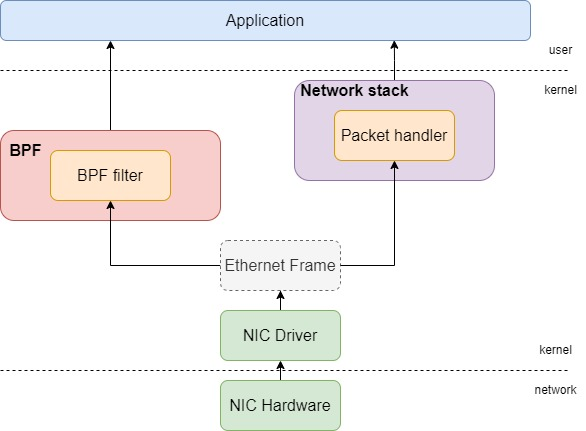
\includegraphics[width=12cm, keepaspectratio=true]{classic_bpf.jpg}
	\caption{Functionality of classic BPF. Based on the figure at the original paper \cite{bpf_bsd_origin_bpf_page2}.}
	\label{fig:classif_bpf}
\end{figure}

Figure \ref{fig:classif_bpf} shows how BPF was integrated in the existing network packet processing by the kernel. After receiving a packet via the Network Interface Controller (NIC) driver, it would first be analysed by BPF filters, which are programs directly developed by the user. This filter decides whether the packet is to be accepted by analysing the packet properties, such as its length or the type and values of its headers. If a packet is accepted, the filter proceeds to decide how many bytes of the original buffer are passed to the application at the user space. Otherwise, the packet is redirected to the original network stack, where it is managed as usual.


\subsection{The BPF virtual machine} \label{subsection:bpf_vm}
In a technical level, BPF comprises both the BPF filter programs developed by the user and the BPF module included in the kernel which allows for loading and running the BPF filters. This BPF module in the kernel works as a virtual machine \cite{bpf_bsd_origin_bpf_page1}, meaning that it parses and interprets the filter program by providing simulated components needed for its execution, turning into a software-based CPU. Because of this reason, it is usually referred as the BPF Virtual Machine (BPF VM). The BPF VM comprises the following components:
\begin{itemize}
\item \textbf{An accumulator register}, used to store intermediate values of operations.
\item \textbf{An index register}, used to modify operand addresses, it is usually incorporated to optimize vector operations \cite{index_register}.
\item \textbf{A scratch memory store}, a temporary storage.
\item \textbf{A program counter}, used to point to the next machine instruction to execute in a filter program.
\end{itemize}


\subsection{Analysis of a BPF filter program} \label{subsection:analysis_bpf_filter_prog}
As we mentioned in Section \ref{subsection:bpf_vm}, the components of the BPF VM are used to support running BPF filter programs. A BPF filter is implemented as a boolean function:
\begin{itemize}
\item If it returns \textit{true}, the kernel copies the packet to the application.
\item If it returns \textit{false}, the packet is not accepted by the filter (and thus the network stack will be the next to operate it).
\end{itemize}

Figure \ref{fig:cbpf_prog} shows an example of a BPF filter upon receiving a packet. In the figure, green lines indicate that the condition is true and red lines that it is evaluated as false. Therefore, the execution works as a control flow graph (CFG) which ends on a boolean value \cite{bpf_bsd_origin_bpf_page5}. The figure presents an example BPF program which accepts the following frames:
\begin{itemize}
\item Frames with an IP packet as a payload directed from IP address X.
\item Frames with an IP packet as a payload directed towards IP address Y.
\item Frames belonging to the ARP protocol and from IP address Y.
\item Frames not from the ARP protocol directed from IP address Y to IP address X.
\end{itemize}

\begin{figure}[ht]
	\centering
	\includegraphics[width=8cm]{cbpf_prog.jpg}
	\caption{Execution of a BPF filter.}
	\label{fig:cbpf_prog}
\end{figure}


\subsection{BPF bytecode instruction format}
In order to implement the CFG to be run at the BPF VM, BPF filter programs are made up of BPF bytecode, which is defined by a new BPF instruction set. Therefore, a BPF filter program is an array of BPF bytecode instructions \cite{bpf_organicprogrammer_analysis}.


\begin{table}[htbp]
\begin{tabular}{|c|c|c|c|c|}
\hline
& \textbf{OPCODE} & \textbf{JT} & \textbf{JF} & \textbf{K}\\
\hline
\textbf{BITS} & 16 & 8 & 8 & 32\\
\hline
\end{tabular}
\caption{BPF instruction format.}
\label{table:bpf_inst_format}
\end{table}

Table \ref{table:bpf_inst_format} shows the format of a BPF bytecode instruction. As it can be observed, it is a fixed-length 64-bit instruction composed of:
\begin{itemize}
\item An \textbf{opcode}, similar to assembly opcode, it indicates the operation to be executed.
\item Field \textbf{jt} indicates the offset to the next instruction to jump in case a condition is evaluated as \textit{true}.
\item Field \textbf{jf} indicates the offset to the next instruction to jump in case a condition is evaluated as \textit{false}.
\item Field \textbf{k} is miscellaneous and its contents vary depending on the instruction opcode.
\end{itemize}

Figure \ref{fig:bpf_instructions} shows how BPF instructions are defined according to the BPF instruction set. As we mentioned, similarly to assembly, instructions include an opcode which indicates the operation to execute, and the multiple arguments defining the arguments of the operation. The table shows, in order by rows, the following instruction types \cite{bpf_bsd_origin_bpf_page8}:
\begin{itemize}
\item Rows 1-4 are \textbf{load instructions}, copying the addressed value into the index or accumulator register.
\item Rows 4-6 are \textbf{store instructions}, copying the accumulator or index register into the scratch memory store.
\item Rows 7-11 are \textbf{jump instructions}, changing the program counter register. These are usually present on each node of the CFG and evaluate whether the condition to be evaluated is true or not.
\item Rows 12-19 and 21-22 are \textbf{arithmetic and miscellaneous instructions}, performing operations usually needed during the program execution.
\item Row 20 is a \textbf{return instruction}, it is positioned in the final end of the CFG, and indicate whether the filter accepts the packet (returning true) or otherwise rejects it (return false).
\end{itemize}

\begin{figure}[htbp]
	\centering
	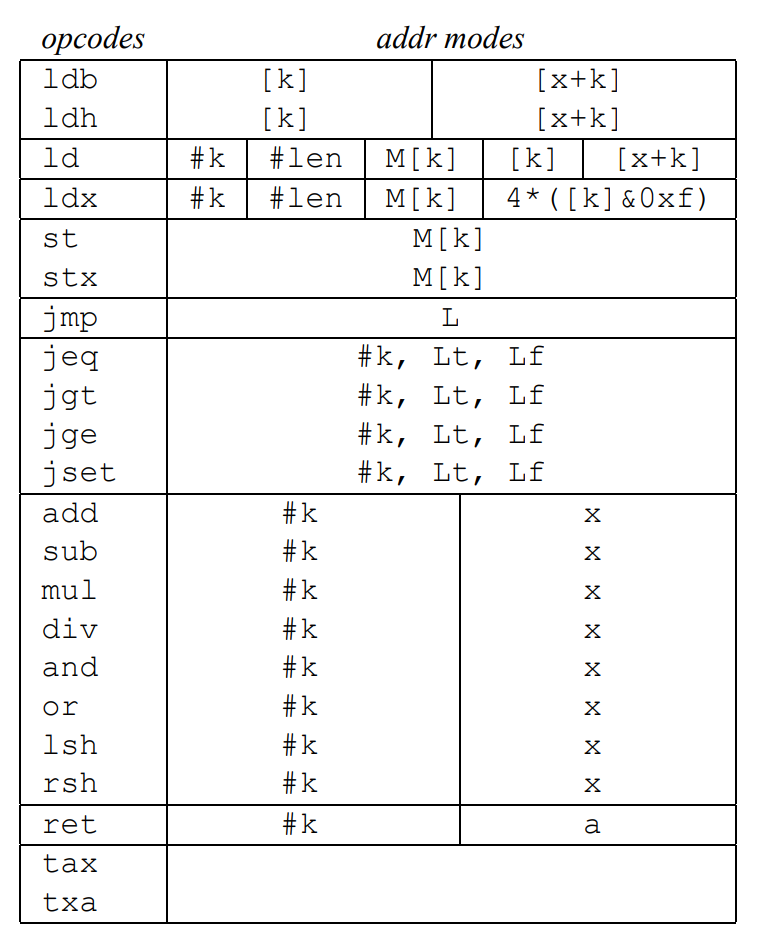
\includegraphics[width=8cm]{bpf_instructions.png}
	\caption{Supported classic BPF instructions, as shown by McCanne and Jacobson \cite{bpf_bsd_origin_bpf_page7}}
	\label{fig:bpf_instructions}
\end{figure}

The column \textit{addr modes} in Figure \ref{fig:bpf_instructions} describes how the parameters of a BPF instruction are referenced depending on the opcode. The address modes are detailed in Figure \ref{fig:bpf_address_mode}. As it can be observed, parameters may consist of immediate values, offsets to memory positions or on the packet, the index register or combinations of the previous.

\begin{figure}[htbp]
	\centering
	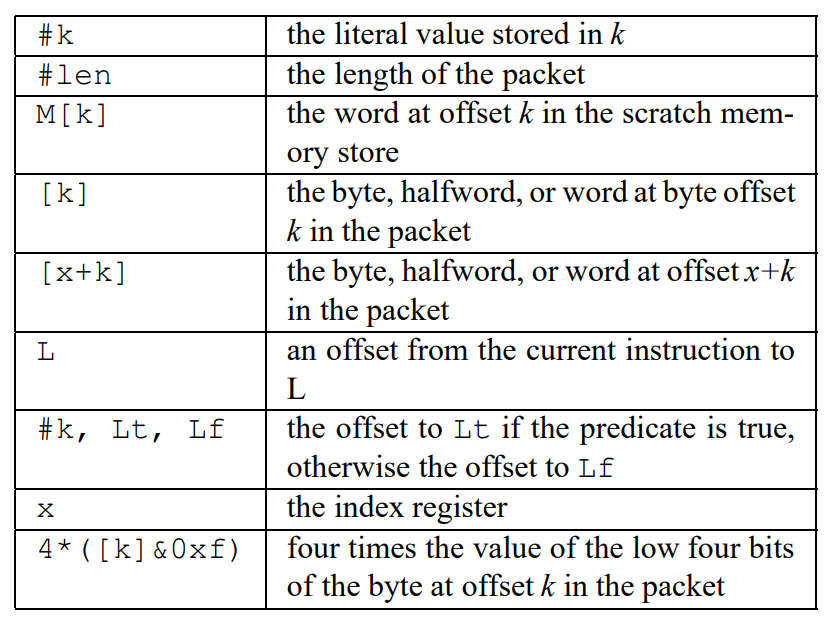
\includegraphics[width=8cm]{bpf_address_mode.png}
	\caption{BPF address modes, as shown by McCanne and Jacobson \cite{bpf_bsd_origin_bpf_page8}}
	\label{fig:bpf_address_mode}
\end{figure}

\subsection{An example of BPF filter with tcpdump} \label{subsection:tcpdump}
At the time, by filtering packets before they are handled by the kernel instead of using a user-level application, BPF offered a performance improvement between 10 and 150 times the state-of-the art technologies of the moment \cite{bpf_bsd_origin_bpf_page1}. Since then, multiple popular tools began to use BPF, such as the network tracing tool \textit{tcpdump} \cite{tcpdump_page}.

\textit{tcpdump} is a command-line tool that enables to capture and analyse the network traffic going through the system. It works by setting filters on a network interface, so that it shows the packets that are accepted by the filter. Still today, \textit{tcpdump} uses BPF for the filter implementation. Figure \ref{fig:bpf_tcpdump_example} shows an example of BPF code used by \textit{tcpdump} to implement a simple filter.

\begin{figure}[htbp]
	\centering
	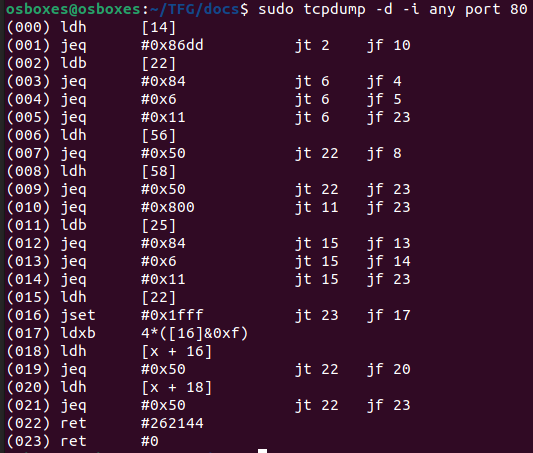
\includegraphics[width=10cm]{tcpdump_example.png}
	\caption{BPF bytecode tcpdump needs to set a filter to display packets directed to port 80.}
	\label{fig:bpf_tcpdump_example}
\end{figure}

In Figure \ref{fig:bpf_tcpdump_example} we can see how tcpdump sets a filter to display traffic directed to all interfaces (\textit{-i any}) directed to port 80. Flag \textit{-d} instructs tcpdump to display BPF bytecode.

In the example, using the \textit{jf} and \textit{jt} fields, we can label the nodes of the CFG described by the BPF filter. Figure \ref{fig:tcpdump_ex_sol} describes the shortest graph path that a true comparison will need to follow to be accepted by the filter. Note how instruction 010 is checking the value 80, the one our filter is looking for in the port.

\begin{figure}[htbp]
	\centering
	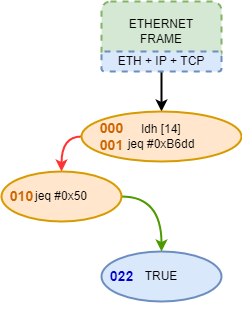
\includegraphics[width=6cm]{cBPF_prog_ex_sol.png}
	\caption{Shortest path in the CFG described in the code shown in Figure \ref{fig:bpf_tcpdump_example} that a packet needs to follow to be accepted by the BPF filter.}
	\label{fig:tcpdump_ex_sol}
\end{figure}

\section{Modern eBPF} \label{section:modern_ebpf}
This section discusses the current state of eBPF in the Linux kernel. By building on the previous architecture described in classic BPF, we will be able to provide a comprehensive picture of the underlying infrastructure in which eBPF relies today.

The addition of classic BPF in the Linux kernel set the foundations of eBPF, but nowadays it has already extended its presence to many other components other than traffic filtering. Similarly to how BPF filters were included in the networking module of the Linux kernel, we will now study the necessary changes made in the kernel to support these new program types. Table \ref{table:ebpf_history} shows the main updates that were incorporated and shaped modern eBPF of today.

\begin{table}[htbp]
\begin{tabular}{|c|c|c|}
\hline
\textbf{DESCRIPTION} & \textbf{KERNEL VERSION} & \textbf{YEAR}\\
\hline
\hline
\textit{BPF}: First addition in the kernel & 2.1.75 & 1997\\
\hline
\textit{BPF+}: New JIT assembler & 3.0 & 2011\\
\hline
\textit{eBPF}: Added eBPF support & 3.15 & 2014\\
\hline
\textit New bpf() syscall & 3.18 & 2014\\
\hline
\textit Introduction of eBPF maps & 3.19 & 2015\\
\hline
\textit eBPF attached to kprobes & 4.1 & 2015\\
\hline
\textit Introduction of Traffic Control & 4.5 & 2016\\
\hline
\textit eBPF attached to tracepoints & 4.7 & 2016\\
\hline
\textit Introduction of XDP & 4.8 & 2016\\
\hline
\end{tabular}
\caption{Relevant eBPF updates. Selection of the official complete table at \cite{ebpf_funcs_by_ver}.}
\label{table:ebpf_history}
\end{table}

As it can be observed in the table above, the main breakthrough happened in the 3.15 version, where Alexei Starovoitov, along with Daniel Borkmann, decided to expand the capabilities of BPF by remodelling the BPF instruction set and overall architecture \cite{brendan_gregg_bpf_book}.

Figure \ref{fig:ebpf_architecture} offers an overview of the current eBPF architecture. During the subsequent subsections, we will proceed to explain its components in detail.

\begin{figure}[htbp]
	\centering
	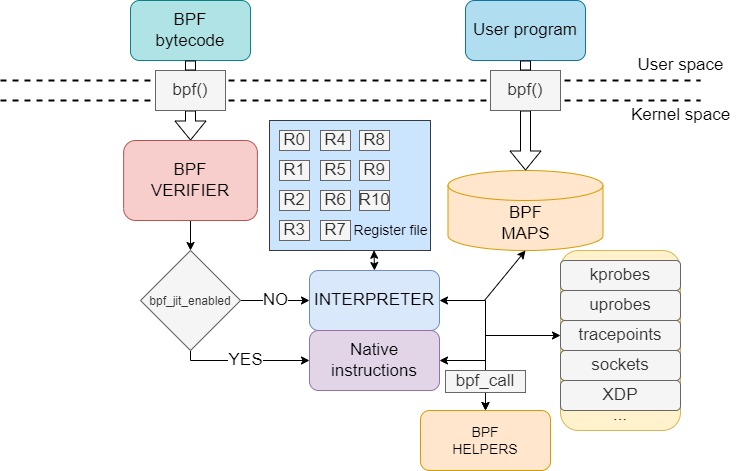
\includegraphics[width=15cm]{ebpf_arch.jpg}
	\caption{eBPF architecture in the Linux kernel and the process of loading an eBPF program. Based on \cite{brendan_gregg_bpf_book} and \cite{ebpf_io_arch}.}
	\label{fig:ebpf_architecture}
\end{figure}

\subsection{eBPF instruction set} \label{subsection:ebpf_inst_set}
The eBPF update included a complete remodel of the instruction set architecture (ISA) of the BPF VM. Therefore, eBPF programs will need to follow the new architecture in order to be interpreted as valid and executed.

Table \ref{table:ebpf_inst_format} shows the new instruction format for eBPF programs \cite{ebpf_inst_set}. As it can be observed, it is a fixed-length 64-bit instruction. The new fields are similar to x86\_64 assembly, incorporating the typically found immediate and offset fields, and source and destination registers \cite{8664_inst_set_specs}. Similarly, the instruction set is extended to be similar to the one typically found on x86\_64 systems, the complete list can be consulted in the official documentation \cite{ebpf_inst_set}.
%Should I talk about assembly or this more in detail?

\begin{table}[htbp]
\begin{tabular}{|c|c|c|c|c|c|}
\hline
& \textbf{IMM} & \textbf{OFF} & \textbf{SRC} & \textbf{DST} & \textbf{OPCODE} \\
\hline
\textbf{BITS} & 32 & 16 & 4 & 4 & 8\\
\hline
\end{tabular}
\caption{eBPF instruction format.}
\label{table:ebpf_inst_format}
\end{table}

With respect to the BPF VM registers, they get extended from 32 to 64 bits of length, and the number of registers is incremented to 10, instead of the original accumulator and index registers. These registers are also adapted to be similar to those in assembly, as it is shown in Table \ref{table:ebpf_regs}.

\begin{table}[htbp]
\begin{tabular}{|>{\centering\arraybackslash}p{2.5cm}|>{\centering\arraybackslash}p{2.5cm}|>{\centering\arraybackslash}p{7cm}|}
\hline
\textbf{eBPF REGISTER} & \textbf{x86\_64 REGISTER} & \textbf{PURPOSE}\\
\hline
\hline
r0 & rax & Return value from functions and exit value of eBPF programs\\
\hline
r1 & rdi & Function call argument 1\\
\hline
r2 & rsi & Function call argument 2\\
\hline
r3 & rdx & Function call argument 3\\
\hline
r4 & rcx & Function call argument 4\\
\hline
r5 & r8 & Function call argument 5\\
\hline
r6 & rbx & Callee saved register, value preserved between calls\\
\hline
r7 & r13 & Callee saved register, value preserved between calls\\
\hline
r8 & r14 & Callee saved register, value preserved between calls\\
\hline
r9 & r15 & Callee saved register, value preserved between calls\\
\hline
r10 & rbp & Frame pointer for stack, read only\\
\hline
\end{tabular}
\caption{eBPF registers and their purpose in the BPF VM. \cite{ebpf_inst_set} \cite{ebpf_starovo_slides}.}
\label{table:ebpf_regs}
\end{table}

\subsection{JIT compilation}
We mentioned in Section \ref{subsection:ebpf_inst_set} that eBPF registers and instructions describe an almost one-to-one correspondence to those in x86 assembly. This is in fact not a coincidence, but rather it is with the purpose of improving a functionality that was included in Linux kernel 3.0, called Just-in-Time (JIT) compilation \cite{ebpf_JIT} \cite{ebpf_JIT_demystify_page13}.

JIT compiling is an extra step that optimizes the execution speed of eBPF programs. It consists of translating BPF bytecode into machine-specific instructions, so that they run as fast as native code in the kernel. Machine instructions are generated during runtime, written directly into executable memory and executed there \cite{ebpf_JIT_demystify_page14}.

Therefore, when using JIT compiling (a setting defined by the variable \textit{bpf\_jit\_enable} \cite{jit_enable_setting}, BPF registers are translated into machine-specific registers following their one-to-one mapping and bytecode instructions are translated into machine-specific instructions \cite{ebpf_starovo_slides_page23}. There no longer exists an interpretation step by the BPF VM, since we can execute the code directly \cite{brendan_gregg_bpf_book_bpf_vm}.

The programs developed during this project will always have JIT compiling active.


\subsection{The eBPF verifier} \label{subsection:ebpf_verifier}
We introduced in Figure \ref{fig:ebpf_architecture} the presence of the so-called eBPF verifier. Provided that we will be loading programs in the kernel from user space, these programs need to be checked for safety before being valid to be executed.

The verifier performs a series of tests which every eBPF program must pass in order to be accepted. Otherwise, user programs could leak privileged data, result in kernel memory corruption, or hang the kernel in an infinite loop, between others. Therefore, the verifier limits multiple aspects of eBPF programs so that they are restricted to the intended functionality, whilst at the same time offering a reasonable amount of freedom to the developer.

The following are the most relevant checks that the verifier performs in eBPF programs \cite{ebpf_verifier_kerneldocs} \cite{ebpf_JIT_demystify_page17-22}:
\begin{itemize}
\item Tests for ensuring overall control flow safety:
	\subitem No loops allowed (bounded loops accepted since kernel version 5.3 \cite{ebpf_bounded_loops}.
	\subitem Function call and jumps safety to known, reachable functions.
	\subitem Sleep and blocking operations not allowed (to prevent hanging the kernel).
\item Tests for individual instructions:
	 \subitem Divisions by zero and invalid shift operations.
	 \subitem Invalid stack access and invalid out-of-bound access to data structures.
	 \subitem Reads from uninitialized registers and corruption of pointers.
\end{itemize}

These checks are performed by two main algorithms:
\begin{itemize}
\item Build a graph representing the eBPF instructions (similar to the one shown in Section \ref{subsection:analysis_bpf_filter_prog}. Check that it is in fact a direct acyclic graph (DAG), meaning that the verifier prevents loops and unreachable instructions.
\item Simulate execution flow by starting on the first instruction and following each possible path, observing at each instruction the state of every register and of the stack.
\end{itemize}

\subsection{eBPF maps} \label{subsection:ebpf_maps}
An eBPF map is a generic storage for eBPF programs used to share data between user and kernel space, to maintain persistent data between eBPF calls and to share information between multiple eBPF programs \cite{ebpf_maps_kernel}.

A map consists of a key + value tuple. Both fields can have an arbitrary data type, the map only needs to know the length of the key and the value field at its creation \cite{bpf_syscall}. Programs can open maps by specifying their ID, and lookup or delete elements in the map by specifying its key, also insert new ones by supplying the element value and they key to store it with.

Therefore, creating a map requires a struct with the fields shown in Table \ref{table:ebpf_map_struct}.

\begin{table}[htbp]
\begin{tabular}{|c|c|}
\hline
\textbf{FIELD} & \textbf{VALUE}\\
\hline
\hline
type & Type of eBPF map. Described in Table \ref{table:ebpf_map_types}\\
\hline
key\_size & Size of the data structure to use as a key\\
\hline
value\_size & Size of the data structure to use as value field\\
\hline
max\_entries & Maximum number of elements in the map\\
\hline
\end{tabular}
\caption{Common fields for creating an eBPF map.}
\label{table:ebpf_map_struct}
\end{table}

Table \ref{table:ebpf_map_types} describes the main types of eBPF maps that are available for use. During the development of our rootkit, we will mainly focus on hash maps (BPF\_MAP\_TYPE\_HASH), provided that they are simple to use and we do not require of any special storage for our research purposes.

\begin{table}[htbp]
\begin{tabular}{|c|>{\centering\arraybackslash}p{7cm}|}
\hline
\textbf{TYPE} & \textbf{DESCRIPTION}\\
\hline
\hline
BPF\_MAP\_TYPE\_HASH & A hast table-like storage, elements are stored in tuples.\\
\hline
BPF\_MAP\_TYPE\_ARRAY & Elements are stored in an array.\\
\hline
BPF\_MAP\_TYPE\_RINGBUF & Map providing alerts from kernel to user space, covered in Section \ref{subsection:bpf_ring_buf}\\
\hline
BPF\_MAP\_TYPE\_PROG\_ARRAY & Stores descriptors of eBPF programs\\
\hline
\end{tabular}
\caption{Relevant types of eBPF maps. Full list can be consulted in the man page \cite{bpf_syscall}}
\label{table:ebpf_map_types}
\end{table}

\subsection{The eBPF ring buffer} \label{subsection:bpf_ring_buf}
eBPF ring buffers are a special kind of eBPF maps, providing a one-way directional communication system, going from an eBPF program in the kernel to a user space program that subscribes to its events.


\subsection{The bpf() syscall} \label{subsection:bpf_syscall}
The bpf() syscall is used to issue commands from user space to kernel space in eBPF programs. This syscall is multiplexor, meaning that it can perform a great range of actions, changing its behaviour depending on the parameters.

The main operations that can be issued are described in Table \ref{table:ebpf_syscall}:

\begin{table}[htbp]
\begin{tabular}{|c|>{\centering\arraybackslash}p{4cm}|>{\centering\arraybackslash}p{4cm}|}
\hline
\textbf{COMMAND} & \textbf{ATTRIBUTES} & \textbf{DESCRIPTION}\\
\hline
\hline
BPF\_MAP\_CREATE & Struct with map info as defined in Table \ref{table:ebpf_map_struct} & Create a new map\\
\hline
BPF\_MAP\_LOOKUP\_ELEM & Map ID, and struct with key to search in the map & Get the element on the map with a specific key\\
\hline
BPF\_MAP\_UPDATE\_ELEM & Map ID, and struct with key and new value & Update the element of an specific key with a new value\\
\hline
BPF\_MAP\_DELETE\_ELEM & Map ID and struct with key to search in the map & Delete the element on the map with an specific key\\
\hline
BPF\_PROG\_LOAD & Struct describing the type of eBPF program to load & Load an eBPF program in the kernel\\
\hline
\end{tabular}
\caption{Relevant types of syscall actions. Full list and attribute details can be consulted in the man page \cite{bpf_syscall}}
\label{table:ebpf_syscall}
\end{table}

With respect to the program type indicated with BPF\_PROG\_LOAD, this parameter indicates the type of eBPF program, setting the context in the kernel in which it will run, and to which modules it will have access to. The types of programs relevant for our research are described in Table \ref{table:ebpf_prog_types}.

\begin{table}[htbp]
\begin{tabular}{|c|>{\centering\arraybackslash}p{5cm}|}
\hline
\textbf{PROGRAM TYPE} & \textbf{DESCRIPTION}\\
\hline
\hline
BPF\_PROG\_TYPE\_KPROBE & Program to instrument code to an attached kprobe\\
\hline
BPF\_PROG\_TYPE\_UPROBE & Program to instrument code to an attached uprobe\\
\hline
BPF\_PROG\_TYPE\_TRACEPOINT & Program to instrument code to a syscall tracepoint\\
\hline
BPF\_PROG\_TYPE\_XDP & Program to filter, redirect and monitor network events from the Xpress Data Path\\
\hline
BPF\_PROG\_TYPE\_SCHED\_CLS & Program to filter, redirect and monitor events using the Traffic Control classifier\\
\hline
\end{tabular}
\caption{Relevant types of eBPF programs. Full list and attribute details can be consulted in the man page \cite{bpf_syscall}.}
\label{table:ebpf_prog_types}
\end{table}

In Section \ref{section:ebpf_prog_types}, we will proceed to analyse in detail the different program types and what capabilities they offer.

\subsection{eBPF helpers} \label{subsection:ebpf_helpers}
Our last component to cover of the eBPF architecture are the eBPF helpers. Since eBPF programs have limited accessibility to kernel functions (which kernel modules commonly have free access to), the eBPF system offers a set of limited functions called helpers \cite{ebpf_helpers}, which are used by eBPF programs to perform certain actions and interact with the context on which they are run. The list of helpers a program can call varies between eBPF program types, since different programs run in different contexts.

It is important to highlight that, just like commands issued via the bpf() syscall can only be issued from the user space, eBPF helpers correspond to the kernel-side of eBPF program exclusively. Note that we will also find a symmetric correspondence to those functions of the bpf() syscall related to map operations (since these are accessible both from user and kernel space).

Table \ref{table:ebpf_helpers} lists the most relevant general-purpose eBPF helpers we will use during the development of our project. We will later detail those helpers exclusive to an specific eBPF program type in the sections on which they are studied.

\begin{table}[htbp]
\begin{tabular}{|c|>{\centering\arraybackslash}p{8cm}|}
\hline
\textbf{eBPF HELPER}& \textbf{DESCRIPTION}\\
\hline
\hline
bpf\_map\_lookup\_elem() & Query an element with a certain key in a map\\
\hline
bpf\_map\_delete\_elem() & Delete an element with a certain key in a map\\
\hline
bpf\_map\_update\_elem() & Update the value of the element with a certain key in a map\\
\hline
bpf\_probe\_read\_user() & Attempt to safely read data at an specific user address into a buffer\\
\hline
bpf\_probe\_read\_kernel() & Attempt to safely read data at an specific kernel address into a buffer\\
\hline
bpf\_trace\_printk() & Similarly to printk() in kernel modules, writes buffer in \/sys\/kernel\/debug\/tracing\/trace\_pipe\\
\hline
bpf\_get\_current\_pid\_tgid() & Get the process' Process Id (PID) and thread group id (TGID)\\
\hline
bpf\_get\_current\_comm() & Get the name of the executable\\
\hline
bpf\_probe\_write\_user() & Attempt to write data at a user memory address\\
\hline
bpf\_override\_return() & Override return value of a probed function\\
\hline
bpf\_ringbuf\_submit() & Submit data to an specific eBPF ring buffer, and notify to subscribers\\
\hline
bpf\_tail\_call() & Jump to another eBPF program preserving the current stack\\
\hline
\end{tabular}
\caption{Relevant common eBPF helpers. Helpers exclusive to an specific program type are not listed. Full list and attribute details can be consulted in the man page \cite{ebpf_helpers}.}
\label{table:ebpf_helpers}
\end{table}


\section{eBPF program types} \label{section:ebpf_prog_types}
In the previous subsection \ref{subsection:bpf_syscall} we introduced the new types of eBPF programs that are supported and that we will be developing for our offensive analysis. In this section, we will analyse in greater detail how eBPF is integrated in the Linux kernel in order to support these new functionalities.

\subsection{XDP} \label{subsection:xdp}
Express Data Path (XDP) programs are a novel type of eBPF program that allows for the lowest-latency traffic filtering and monitoring in the whole Linux kernel. In order to load an XDP program, a bpf() syscall with the command BPF\_PROG\_LOAD and the program type BPF\_PROG\_TYPE\_XDP must be issued. 

These programs are directly attached to the Network Interface Controller (NIC) driver, and thus they can process the packet before any other module \cite{xdp_gentle_intro}.

Figure \ref{fig:xdp_diag} shows how XDP is integrated in the network processing of the Linux kernel. After receiving a raw packet (in the figure, \textit{xdp\_md}, which consists on the raw bytes plus some very basic metadata about the packet) from the incoming traffic, XDP program can perform the following actions \cite{xdp_manual}:
\begin{itemize}
\item Analyse the data between the packet buffer bounds.
\item Modify the packet contents, and modify the packet length.
\item Decide between one of the actions displayed in Table \ref{table:xdp_actions_av}.
\end{itemize}

\begin{figure}[htbp]
	\centering
	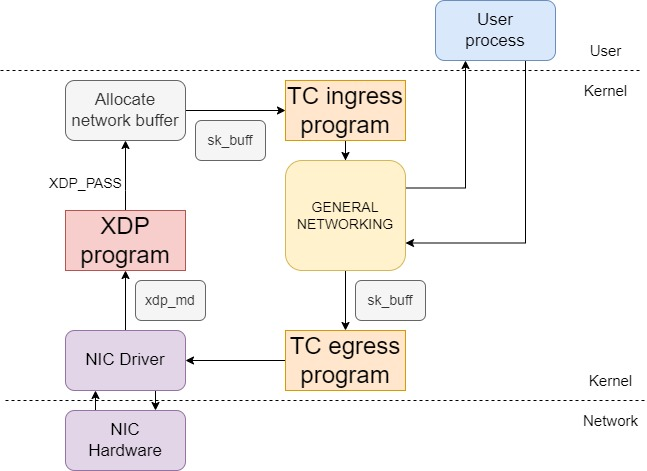
\includegraphics[width=15cm]{xdp_diag.jpg}
	% Either this caption, or change the text afterwards. I still need to know whether to put the long explanation here or on the paragraph, it gets repetitive.
	\caption{XDP and TC modules integration in the network processing module of the Linux kernel.}
	\label{fig:xdp_diag}
\end{figure}

\begin{table}[htbp]
\begin{tabular}{|c|>{\centering\arraybackslash}p{10cm}|}
\hline
\textbf{ACTION} & \textbf{DESCRIPTION}\\
\hline
\hline
XDP\_PASS & Let packet proceed with operated modifications on it.\\
\hline
XDP\_TX & Return the packet at the same NIC it was received from. Packet modifications are kept.\\
\hline
XDP\_DROP & Drops the packet completely, kernel networking will not be notified.\\
\hline
\end{tabular}
\caption{Relevant XDP return values.}
\label{table:xdp_actions_av}
\end{table}

Some of the XDP-exclusive eBPF helpers we will be discussing in later sections are shown in Table \ref{table:xdp_helpers}.
\begin{table}[htbp]
\begin{tabular}{|c|>{\centering\arraybackslash}p{8cm}|}
\hline
\textbf{eBPF HELPER} & \textbf{DESCRIPTION}\\
\hline
\hline
bpf\_xdp\_adjust\_head() & Enlarges or reduces the extension of a packet, by moving the address of its first byte.\\
\hline
bpf\_xdp\_adjust\_tail() & Enlarges or reduces the extension of a packet, by moving the address of its last byte.\\
\hline
\end{tabular}
\caption{Relevant XDP-exclusive eBPF helpers.}
\label{table:xdp_helpers}
\end{table}


\subsection{Traffic Control} \label{subsection:tc}
Traffic Control (TC) programs are also indicated for networking instrumentation. Similarly to XDP, their module is positioned before entering the overall network processing of the kernel. However, as it can be observed in Figure \ref{fig:xdp_diag}, they differ in some aspects:
\begin{itemize}
\item TC programs receive a network buffer with metadata (in the figure, \textit{sk\_buff}) about the packet in it. This renders TC programs less ideal than XDP for performing large packet modifications (like new headers), but at the same time the additional metadata fields make it easier to locate and modify specific packet fields \cite{tc_differences}.
\item TC programs can be attached to the \textit{ingress} or \textit{egress} points, meaning that an eBPF program can operate not only over incoming traffic, but also over the outgoing packets.
\end{itemize}

With respect to how TC programs operate, the Traffic Control system in Linux is greatly complex and would require a complete section by itself. In fact, it was already a complete system before the appearance of eBPF. Full documentation can be found at \cite{tc_docs_complete}. For this document, we will explain the overall process needed to load a TC program \cite{tc_direct_action}:
\begin{enumerate}
\item The TC program defines a so-called queuing discipline (qdisc), a packet scheduler that issues packets in a First-In-First-Out (FIFO) order as soon as they are received. This qdisc will be attached to a specific network interface (e.g.: wlan0).
\item Our TC eBPF program is attached to the qdisc. It will work as a filter, being run for every of the packets dispatched by the qdisc.
\end{enumerate}

Similarly to XDP, the TC eBPF programs can decide an action to be executed on a packet by specifying a return value. These actions are almost analogous to the ones in XDP, as it can be observed in Table \ref{table:tc_actions}.

\begin{table}[htbp]
\begin{tabular}{|c|>{\centering\arraybackslash}p{9cm}|}
\hline
\textbf{ACTION} & \textbf{DESCRIPTION}\\
\hline
\hline
TC\_ACT\_OK & Let packet proceed with operated modifications on it.\\
\hline
TC\_ACT\_RECLASSIFY & Return the packet to the back of the qdisc scheduling queue.\\
\hline
TC\_ACT\_SHOT & Drops the packet completely, kernel networking will not be notified.\\
\hline
\end{tabular}
\caption{Relevant TC return values. Full list can be consulted at \cite{tc_ret_list_complete}.}
\label{table:tc_actions}
\end{table}

Finally, as in XDP, there exists a list of useful BPF helpers that will be relevant for the creation of our rootkit. They are shown in Table \ref{table:tc_helpers}.
\begin{table}[htbp]
\begin{tabular}{|c|>{\centering\arraybackslash}p{9cm}|}
\hline
\textbf{eBPF HELPER} & \textbf{DESCRIPTION}\\
\hline
\hline
bpf\_l3\_csum\_replace() & Recomputes the network layer 3 (e.g.: IP) checksum of the packet.\\
\hline
bpf\_l4\_csum\_replace() & Recomputes the network layer 4 (e.g.: TCP) checksum of the packet.\\
\hline
bpf\_skb\_store\_bytes() & Write a data buffer into the packet.\\
\hline
bpf\_skb\_pull\_data() & Reads a sequence of packet bytes into a buffer.\\
\hline
bpf\_skb\_change\_head() & (Only) enlarges the extension of a packet, by moving the address of its first byte.\\
\hline
bpf\_skb\_change\_tail() & Enlarges or reduces the extension of a packet, by moving the address of its last byte.\\
\hline
\end{tabular}
\caption{Relevant TC-exclusive eBPF helpers.}
\label{table:tc_helpers}
\end{table}

\subsection{Tracepoints} \label{subsection:tracepoints}
Tracepoints are a technology in the Linux kernel that allows to hook functions in the kernel, connecting a 'probe': a function that is executed every time the hooked function is called \cite{tp_kernel}. These tracepoints are set statically during kernel development, meaning that for a function to be hooked, it needs to have been previously marked with a tracepoint statement indicating its traceability. At the same time, this limits the number of tracepoints available.

The list of tracepoint events available depends on the kernel version and can be visited under the directory \textit{/sys/kernel/debug/tracing/events}.

It is particularly relevant for our later research that most of the system calls incorporate a tracepoint, both when they are called (\textit{enter} tracepoint) and when they are exited (\textit{exit} tracepoints). This means that, for a system call sys\_open, both the tracepoint sys\_enter\_open and sys\_exit\_open are available. 

Also, note that the probe functions that are called when hitting a tracepoint receive some parameters related to the context on which the tracepoint is located. In the case of syscalls, these include the parameters with which the syscall was called (only for \textit{enter} syscalls, \textit{exit} ones will only have access to the return value). The exact parameters and their format which a probe function receives can be visited in the file \textit{/sys/kernel/debug/tracing/events/<subsystem>/<tracepoint>/format}. In the previous example with sys\_enter\_open, this is \textit{/sys/kernel/debug/tracing/events/syscalls/sys\_enter\_open/format}.

In eBPF, a program can issue a bpf() syscall with the command BPF\_PROG\_LOAD and the program type BPF\_PROG\_TYPE\_TRACEPOINT, specifying which is the function with the tracepoint to attach to and an arbitrary function probe to call when it is hit. This function probe is defined by the user in the eBPF program submitted to the kernel.

\subsection{Kprobes}
Kprobes are another tracing technology of the Linux kernel whose functionality has been become available to eBPF programs. Similarly to tracepoints, kprobes enable to hook functions in the kernel, with the only difference that it is dynamically attached to any arbitrary function, rather than to a set of predefined positions \cite{kprobe_manual}. It does not require that kernel developers specifically mark a function to be probed, but rather kprobes can be attached to any instruction, with a short list of blacklisted exceptions. 

As it happened with tracepoints, the probe functions have access to the parameters of the original hooked function. Also, the kernel maintains a list of kernel symbols (addresses) which are relevant for tracing and that offer us insight into which functions we can probe. It can be visited under the file \textit{/proc/kallsyms}, which exports symbols of kernel functions and loaded kernel modules \cite{kallsyms_kernel}.

Also similarly, since tracepoints could be found in their \textit{enter} and \textit{exit} variations, kprobes have their counterpart, named kretprobes, which call the hooked probe once a return instruction is reached after the hooked symbol. This means that a kretprobe hooked to a kernel function will call the probe function once it exits.

In eBPF, a program can issue a bpf() syscall with the command BPF\_PROG\_LOAD and the program type BPF\_PROG\_TYPE\_KPROBE, specifying which is the function with the kprobe to attach to and an arbitrary function probe to call when it is hit. This function probe is defined by the user in the eBPF program submitted to the kernel.

\subsection{Uprobes}
Uprobes is the last of the main tracing technologies which has been become accessible to eBPF programs. They are the counterparts of Kprobes, allowing for tracing the execution of an specific instruction in the user space, instead of in the kernel. When the execution flow reaches a hooked instruction, a probe function is run. 

For setting an uprobe on a specific instruction of a program, we need to know three components:
\begin{itemize}
\item The name of the program.
\item The address of the function where the instruction is contained.
\item The offset at which the specific instruction is placed from the start of the function.
\end{itemize}

Similarly to kprobes, uprobes have access to the parameters received by the hooked function. Also, the complementary uretprobes exist too, running the probe function once the hooked function returns.

In eBPF, programs can issue a bpf() syscall with the command BPF\_PROG\_LOAD and the program type BPF\_PROG\_TYPE\_UPROBE, specifying the function with the uprobe to attach to and an arbitrary function probe to call when it is hit. This function probe is also defined by the user in the eBPF program submitted to the kernel.

\section{Developing eBPF programs}
In Section \ref{section:modern_ebpf}, we discussed the overall architecture of the eBPF system which is now an integral part of the Linux kernel. We also studied the process which a piece of eBPF bytecode follows in order to be accepted in the kernel. However, for an eBPF developer, programming bytecode and working with bpf() calls natively is not an easy task, therefore an additional layer of abstraction was needed. 

Nowadays, there exist multiple popular alternatives for writing and running eBPF programs. We will overview which they are and proceed to analyse in further detail the option that we will use for the development of our rootkit.

\subsection{BCC}
BPF Compiler Collection (BCC) is one of the first and well-known toolkits for eBPF programming available \cite{bcc_github}. It allows to include eBPF code into user programs. These programs are developed in Python, and the eBPF code is embedded as a plain string.

Although BCC offers a wide range of tools to easy the development of eBPF programs, we found it not to be the most appropriate for our large-scale eBPF project. In particular, this was due to the feature of eBPF programs being stored as a python string, which leads to difficult scalability, poor development experience given that programming errors are detected at runtime (once the python program issues the compilation of the string), and simply better features from competing libraries.

\subsection{Bpftool}
Bpftool is not a development framework like BCC, but one of the most relevant tools for eBPF program development. Some of its functionalities include:
\begin{itemize}
\item Loading eBPF programs.
\item List running eBPF programs.
\item Dumping bytecode from live eBPF programs.
\item Extract program statistics and data from programs.
\item List and operate over eBPF maps.
\end{itemize}

Although we will not be covering bpftool during our overview on the constructed eBPF rootkit, it was used extensively during the development and became a key tool for debugging eBPF programs, particularly to peek data at eBPF maps during runtime.

\subsection{Libbpf} \label{subsection:libbpf}
Libbpf \cite{libbpf_github} is a library for loading and interacting with eBPF programs, which is currently maintained in the Linux kernel source tree \cite{libbpf_upstream}. It is one of the most popular frameworks to develop eBPF applications, both because it makes eBPF programming similar to common kernel development and because it aims at reducing kernel-version dependencies, thus increasing programs portability between systems \cite{libbpf_core}. During our research, however, we will not make use of this functionalities given that a portable program is not in our research goals.

As we discussed in Section \ref{section:modern_ebpf}, eBPF programs are composed of both the eBPF code in the kernel and a user space program that can interact with it. With libbpf, the eBPF kernel program is developed in C (a real program, not a string later compiled as with BCC), while user programs are usually developed in C, Rust or GO. For our project, we will use the C version of libbpf, so both the user and kernel side of our rootkit will be developed in this language.

When using libbpf with the C language, both the user-side and kernel eBPF program are compiled together using the Clang/LLVM compiler, translating C instructions into eBPF bytecode. As a clarification, Clang is the front-end of the compiler, translating C instructions into an intermediate form understandable by LLVM, whilst LLVM is the back end compiling the intermediate code into eBPF bytecode. As it can be observed in Figure \ref{fig:libbpf}, the result of the compilation is a single program, comprising the user-side which will launch a user process, the eBPF bytecode to be run in the kernel, and other structures libbpf generates about eBPF maps and other meta data. This program is encapsulated as an ELF file (a common executable format).

\begin{figure}[htbp]
	\centering
	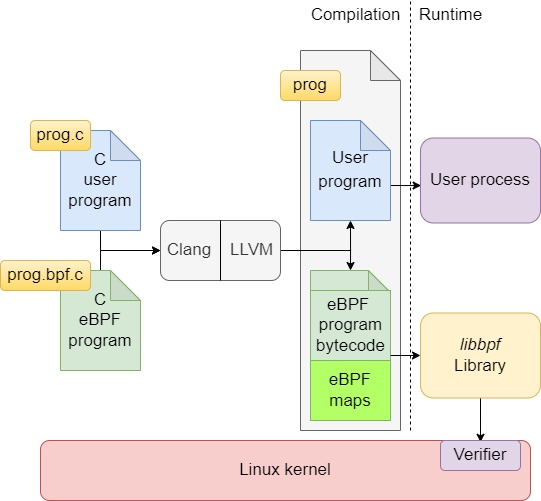
\includegraphics[width=12cm, keepaspectratio=true]{libbpf_prog.jpg}
	\caption{Compilation and loading process of a program developed with libbpf.}
	\label{fig:libbpf}
\end{figure}

Finally, we will overview one of the main functionalities of libbpf to simplify eBPF programming, namely the BPF skeleton. This is auto-generated code by libbpf whose aim is to simplify working with eBPF from the user-side program. As a summary, it parses the eBPF programs developed (which may be using different technologies such as XDP, kprobes, TC...) and the eBPF maps used, and as a result offers a simple set of functions for dealing with these programs from the user program. In particular, it allows for loading and unloading a specific eBPF program from user space at runtime.

Table \ref{table:libbpf_skel} describes the API offered by the BPF skeleton. Note that <name> is substituted by the name of the program being compiled.

\begin{table}[htbp]
\begin{tabular}{|c|>{\centering\arraybackslash}p{9cm}|}
\hline
\textbf{FUNCTION NAME} & \textbf{DESCRIPTION}\\
\hline
\hline
<name>\_\_open() & Parse the eBPF programs and maps.\\
\hline
<name>\_\_load() & Load the eBPF map in the kernel after its validation, create the maps. However, the programs are not active yet.\\
\hline
<name>\_\_attach() & Activate the eBPF programs, attaching them to their corresponding parts in the kernel (e.g. kprobes to kernel functions).\\
\hline
<name>\_\_destroy() & Detach and unload the eBPF programs from the kernel.\\
\hline
\end{tabular}
\caption{BPF skeleton functions.}
\label{table:libbpf_skel}
\end{table}

Note that the BPF skeleton also offers further granularity at the time of dealing with programs, so that individual programs can be loaded or attached instead of all simultaneously. This is the approach we will generally use in the development of our rootkit, as it will be explained in Section \ref{subsection:ebpf_progs_config}.



\section{Security features in eBPF} \label{section:ebpf_security}
As we have shown in Section \ref{section:modern_ebpf}, eBPF has been an active part of the Linux kernel from its 3.18 version. However, as with many other components of the kernel, its availability to the user depends on the parameters with which the kernel has been compiled. Specifically, eBPF is only available to kernels compiled with the flags specified in Table \ref{table:ebpf_kernel_flags}.

\begin{table}[htbp]
\begin{tabular}{|c|c|>{\centering\arraybackslash}p{7cm}|}
\hline
\textbf{FLAG} & \textbf{VALUE} & \textbf{DESCRIPTION}\\
\hline
\hline
\multicolumn{1}{|c|}{CONFIG\_BPF} & \multicolumn{1}{c|}{y} & \multirow{2}{*}{Basic BPF compilation (mandatory)}\\
\cline{1-2}
\multicolumn{1}{|c|}{CONFIG\_BPF\_SYSCALL} & \multicolumn{1}{c|}{m} & \\
\hline
\multicolumn{1}{|c|}{CONFIG\_NET\_ACT\_BPF} & \multicolumn{1}{c|}{m} & \multirow{2}{*}{Traffic Control functionality}\\
\cline{1-2}
\multicolumn{1}{|c|}{CONFIG\_NET\_CLS\_BPF} & \multicolumn{1}{c|}{y} & \\
\hline
\multicolumn{1}{|c|}{CONFIG\_BPF\_JIT} & \multicolumn{1}{c|}{y} & \multirow{2}{*}{Enable JIT compliation}\\
\cline{1-2}
\multicolumn{1}{|c|}{CONFIG\_HAVE\_BPF\_JIT} & \multicolumn{1}{c|}{y} & \\
\hline
\multicolumn{1}{|c|}{CONFIG\_BPF\_EVENTS} & \multicolumn{1}{c|}{y} & \multirow{4}{*}{Enable kprobes, uprobes and tracepoints}\\
\cline{1-2}
\multicolumn{1}{|c|}{CONFIG\_KPROBE\_EVENTS} & \multicolumn{1}{c|}{y} & \\
\cline{1-2}
\multicolumn{1}{|c|}{CONFIG\_UPROBE\_EVENTS} & \multicolumn{1}{c|}{y} & \\
\cline{1-2}
\multicolumn{1}{|c|}{CONFIG\_TRACING} & \multicolumn{1}{c|}{y} & \\
\hline
CONFIG\_XDP\_SOCKETS & y & Enable XDP\\
\hline
\end{tabular}
\caption{Kernel compilation flags for eBPF.}
\label{table:ebpf_kernel_flags}
\end{table}

Table \ref{table:ebpf_kernel_flags} is based on BCC's documentation, but the full list of eBPF-related flags can be extracted in a live system via bpftool, as detailed in \nameref{annex:bpftool_flags_kernel}. Nowadays, all mainstream Linux distributions include kernels with full support for eBPF.


\subsection{Access control} \label{subsection:access_control}
It must be noted that, similarly to kernel modules, loading an eBPF program requires privileged access in the system. In old kernel versions, this means either a user having full root permissions, or having the Linux capability \cite{ubuntu_caps} CAP\_SYS\_ADMIN. Therefore, there existed two main options:

\begin{itemize}
\item \textbf{Privileged users} can load any kind of eBPF program and use any functionality.
\item \textbf{Unprivileged users} can only load and attach eBPF programs of type BPF\_PROG\_TYPE\_SOCKET\_FILTER \cite{evil_ebpf_p9}, offering the very limited functionality of filtering packets received on a socket.
\end{itemize}

More recently, in an effort to further granulate the permissions needed for loading, attaching and running eBPF programs, CAP\_SYS\_ADMIN has been substituted by more specific capabilities \cite{ebpf_caps_intro} \cite{ebpf_caps_lwn}. The current system is therefore described in Table \ref{table:ebpf_caps_current}.

\begin{table}[htbp]
\begin{tabular}{|>{\centering\arraybackslash}p{4cm}|>{\centering\arraybackslash}p{10cm}|}
\hline
\textbf{CAPABILITIES} & \textbf{eBPF FUNCTIONALITY}\\
\hline
\hline
No capabilities & Load and attach BPF\_PROG\_TYPE\_SOCKET\_FILTER, load BPF\_PROG\_TYPE\_CGROUP\_SKB programs.\\
\hline
CAP\_BPF & Load (but not attach) any type of program, create most types of eBPF map and access them if their id is known\\
\hline
CAP\_NET\_ADMIN & Attach networking programs (Traffic Control, XDP, ...)\\
\hline
CAP\_PERFMON & Attaching kprobes, uprobes and tracepoints. Read access to kernel memory.\\
\hline
CAP\_SYS\_ADMIN & Privileged eBPF. Includes iterating over eBPF maps, and CAP\_BPF, CAP\_NET\_ADMIN, CAP\_PERFMON functionalities.\\
\hline
\end{tabular}
\caption{Capabilities needed for eBPF.}
\label{table:ebpf_caps_current}
\end{table}

Therefore, eBPF network programs usually require both CAP\_BPF and CAP\_NET\_ADMIN, whilst tracing programs require CAP\_BPF and CAP\_PERFMON. CAP\_SYS\_ADMIN remains as the (non-preferred) capability to assign to eBPF programs with complete access in the system.

Although for a long time there have existed efforts towards enhancing unprivileged eBPF, it remains a worrying feature \cite{unprivileged_ebpf}. The main issue is that the verifier must be prepared to detect any attempt to extract kernel memory access or user memory modification by unprivileged eBPF programs, which is a complex task. In fact, there have existed numerous security vulnerabilities which allow for privilege escalation using eBPF, that is, execution of privileged eBPF programs by exploiting vulnerabilities in unprivileged eBPF \cite{cve_unpriv_ebpf}.

This influx of security vulnerabilities leads to the recent inclusion of an attribute into the kernel which allows for setting whether unprivileged eBPF is allowed in the system or not. This parameter is named \textit{kernel.unprivileged\_bpf\_disabled}, its values can be seen in Table \ref{table:unpriv_ebpf_values}.

\begin{table}[htbp]
\begin{tabular}{|>{\centering\arraybackslash}p{4cm}|>{\centering\arraybackslash}p{10cm}|}
\hline
\textbf{Value} & \textbf{Meaning}\\
\hline
\hline
0 & Unprivileged eBPF is enabled.\\
\hline
1 & Unprivileged eBPF is disabled. A system reboot is needed to enable it after changing this value.\\
\hline
2 & Unprivileged eBPF is disabled. A system reboot is not needed to enable it after changing this value.\\
\hline
\end{tabular}
\caption{Values for unprivileged eBPF kernel parameter.}
\label{table:unpriv_ebpf_values}
\end{table}

Nowadays, most Linux distributions have set value 1 to this parameter, therefore disallowing unprivileged eBPF completely. These include Ubuntu \cite{unpriv_ebpf_ubuntu}, Suse Linux \cite{unpriv_ebpf_suse} or Red Hat Linux \cite{unpriv_ebpf_redhat}, between others.



\section{Memory management in Linux}
Multiple of the techniques incorporated in our rootkit require a deep understanding into how memory is managed in a Linux process. Therefore, in this section we will present all the background about memory management needed for our later discussion of the offensive capabilities of eBPF in this context.

\subsection{Memory pages and faults} \label{subsection:mem_faults}
Linux systems divide the available random-access memory (RAM) into 'pages', subsections of an specific length, usually 4 KB. The collection of all pages is called physical memory.

Likewise, individual memory sections need to be assigned to each running process in the system, but instead of assigning a set of pages from physical memory, a new address space is defined, named virtual memory, which is divided into pages as well. These virtual memory pages are related to physical memory pages via a page table, so that each virtual memory address of a process can be translated into a real, physical memory address in RAM \cite{mem_page_arch}. Figure \ref{fig:mem_arch_pages} shows a diagram of the described architecture.

\begin{figure}[htbp]
	\centering
	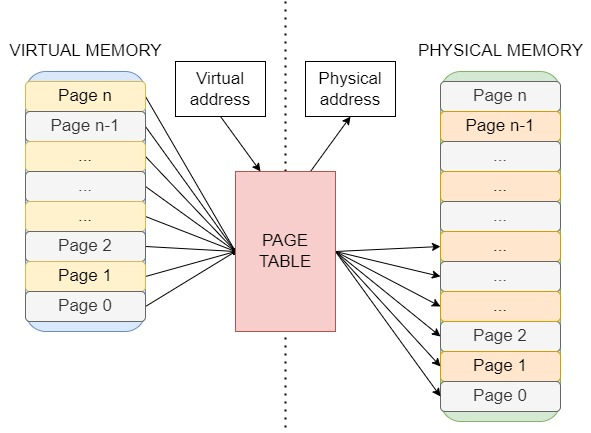
\includegraphics[width=13cm]{mem_arch_pages.jpg}
	\caption{Memory translation of virtual pages to physical pages.}
	\label{fig:mem_arch_pages}
\end{figure}

As we can observe in the figure, each virtual page is related to one physical page. However, RAM needs to maintain multiple processes and data simultaneously, and therefore sometimes the operating system (OS) will remove them from physical memory when it believes they are no longer being used. This leads to the occurrence of two type of memory events \cite{page_faults}:
\begin{itemize}
\item \textbf{Major page faults} occur when a process tries to access a virtual page, but the related physical page has been removed from RAM. In this case, the OS will need to request a secondary storage (such as a hard disk) for the data removed and allocate a new physical page for the virtual page. Figure \ref{fig:mem_major_page_fault} illustrates a major page fault.
\begin{figure}[htbp]
	\centering
	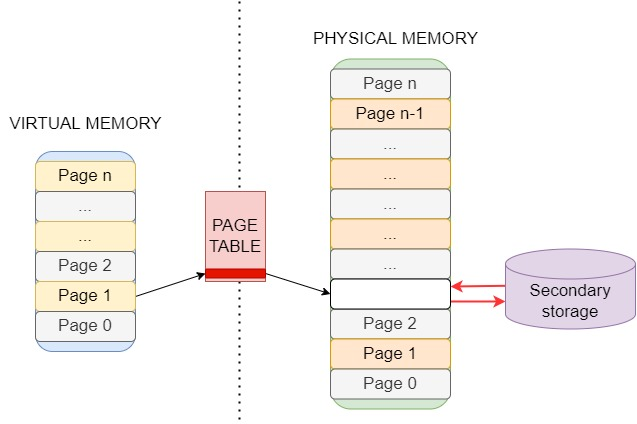
\includegraphics[width=11cm]{mem_major_page_fault.jpg}
	\caption{Major page fault after a page was removed from RAM.}
	\label{fig:mem_major_page_fault}
\end{figure}
\item \textbf{Minor page faults} occur when a process tries to access a virtual page, and although the related physical page exists, the connection in the page table has not been completed. A common event when these fault happen is on fork() calls, since with the purpose of making the call more efficient, the page table of the parent is not always completely copied into the child, leading into multiple minor page faults once the child tries to access the data on them. Figure \ref{fig:mem_minor_page_fault} illustrates a minor page fault after a fork.
\end{itemize}
\begin{figure}[htbp]
	\centering
	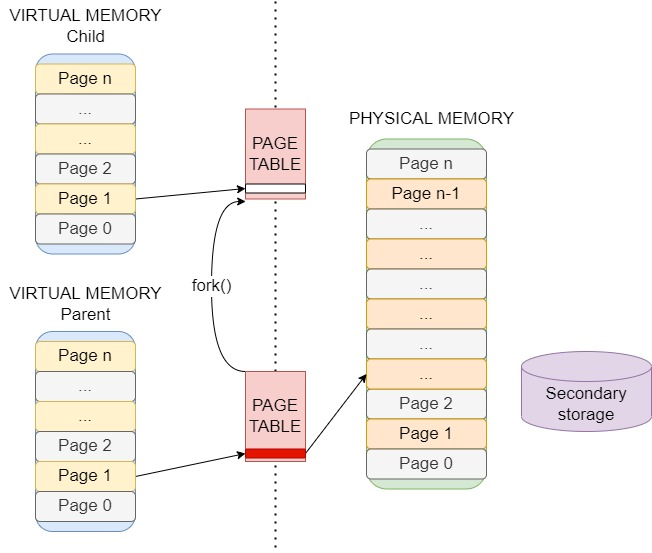
\includegraphics[width=11cm]{mem_minor_page_fault.jpg}
	\caption{Minor page fault after a fork() in which the page table was not copied completely.}
	\label{fig:mem_minor_page_fault}
\end{figure}

\subsection{Process virtual memory}
In the previous subsection we have studied that each process disposes of a virtual address space. We will now describe how this virtual memory is organized in a Linux system.

Figure \ref{fig:mem_proc_arch} describes how virtual memory is distributed within a process in the x86\_64 architecture. As we can observe, it is partitioned into multiple sections:
\begin{figure}[htbp]
	\centering
	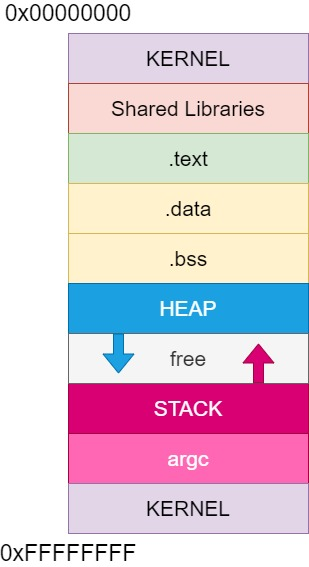
\includegraphics[width=6cm]{memory.jpg}
	\caption{Virtual memory architecture of a process \cite{mem_arch_proc}.}
	\label{fig:mem_proc_arch}
\end{figure}
\begin{itemize}
\item Lower and upper memory addresses are reserved for the kernel.
\item A section where shared libraries code is stored.
\item A .text section, which contains the code of the program being run.
\item A .data section, containing initialized static and global variables.
\item A .bss section, which contains global and static variables which are uninitialized or initialized to zero.
\item The heap, a section which grows from lower to higher memory addresses, and which contains memory dynamically allocated by the program.
\item The stack, a section which grows from higher to lower memory addresses, towards the heap. It is a Last In First Out (LIFO) structure used to store local variables, function parameters and return addresses.
\item Right at the start of the stack we can find the arguments with which the programs has been executed.
\end{itemize}

\subsection{The process stack} \label{subsection:stack}
Among all the sections we identified in a process virtual memory, the stack will be particularly relevant during our research. We will therefore study it now in detail. 

Firstly, we will present how the stack is structured, and which operations can be executed on it. Figure \ref{fig:stack_pres} presents a stack during the execution of a program. Table \ref{table:systemv_abi_other} explains the purpose of the most relevant registers related to the stack and program execution:

\begin{figure}[htbp]
	\centering
	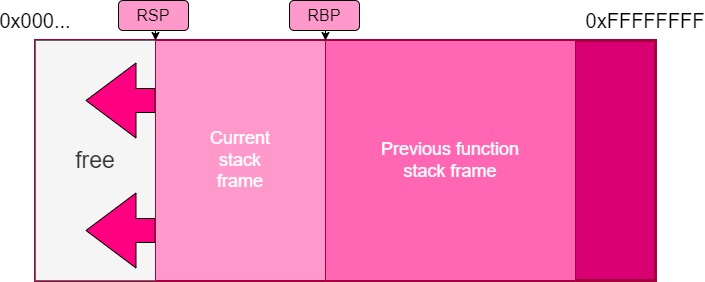
\includegraphics[width=14cm]{stack_pres.jpg}
	\caption{Simplified stack representation showing only stack frames.}
	\label{fig:stack_pres}
\end{figure}

\begin{table}[htbp]
\begin{tabular}{|>{\centering\arraybackslash}p{2cm}|>{\centering\arraybackslash}p{10cm}|}
\hline
\textbf{REGISTER} & \textbf{PURPOSE}\\
\hline
\hline
rip & Instruction Pointer - Memory address of the next instruction to execute\\
\hline
rsp & Stack Pointer - Memory address where next stack operation takes place\\
\hline
rbp & Base/Frame Pointer - Memory address of the start of the stack frame\\
\hline
\end{tabular}
\caption{Relevant registers in x86\_64 for the stack and control flow and their purpose.}
\label{table:systemv_abi_other}
\end{table}

As it can be observed in Figure \ref{fig:stack_pres}, the stack grows towards lower memory addresses, and it is organized in stack frames, delimited by the registers rsp and rbp. An stack frame is a division of the stack which contains all the data (variables, call arguments...) belonging to a single function execution. When a function is exited, its stack frame is removed, and if a function calls a nested function, then its stack frame is preserved and a new stack frame is inserted into the stack. 

As Table \ref{table:systemv_abi_other} explains, the rbp and rsp registers are used for keeping track of the starting and final position of the current stack frame respectively. We can see in Figure \ref{fig:stack_pres} that their value is a memory address pointing to their stack positions. On the other hand, the rip register does not point to the stack, but rather to the .text section (see Figure \ref{fig:mem_proc_arch}), where it points to the next instruction to be executed. However, as we will now see, its value must also be stored in the stack frame when a nested function is called, since after the nested function exits we need to restore the execution in the same instruction of the original function.

As with any LIFO structure, the stack supports two main operations: \textit{push} and \textit{pop}. In the x86\_64 architecture, it operates with chunks of data of either 16, 32 or 64 bytes. Table \ref{fig:stack_ops} shows a representation of these operations in the stack.
\begin{itemize}
\item A \textbf{push} operation writes data in the free memory pointed by register rsp. It then moves the value of rsp to point to the new end of the stack.
\item A \textbf{pop} operation moves the value of rsp by 16, 32 or 64 bytes, and reads the data previously saved in that position.
\end{itemize}

\begin{figure}[htbp]
	\centering
	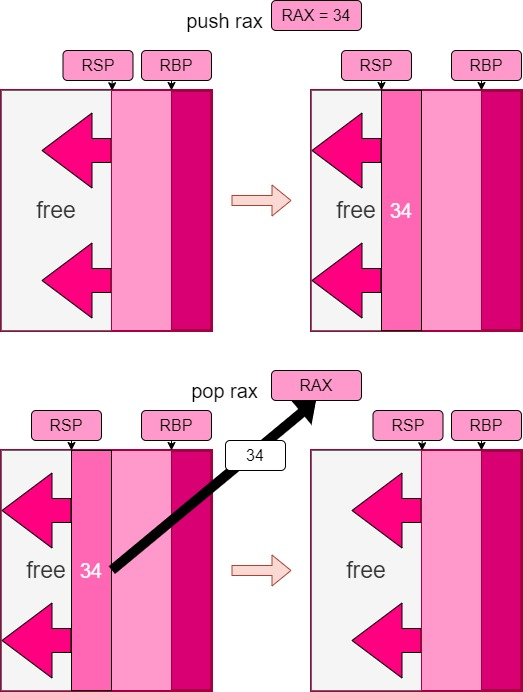
\includegraphics[width=10cm]{stack_ops.jpg}
	\caption{Representation of push and pop operations in the stack.}
	\label{fig:stack_ops}
\end{figure}


As we mentioned, the stack stores function parameters, return addresses and local variables inside a stack frame. We will now study how the processor uses the stack in order to call, execute, and exit a function. To illustrate this process, we will simulate the execution of function \lstinline{func(char* a, char* b, char* c)} \lstinline{}. Figures \ref{fig:stack_before} and \ref{fig:stack} show a representation of the stack during these operations.

\begin{figure}[htbp]
	\centering
	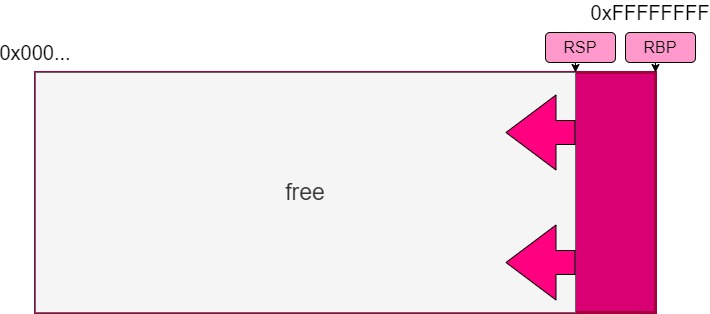
\includegraphics[width=14cm]{stack_before.jpg}
	\caption{Stack representation right before starting the function call process.}
	\label{fig:stack_before}
\end{figure}

\begin{figure}[htbp]
	\centering
	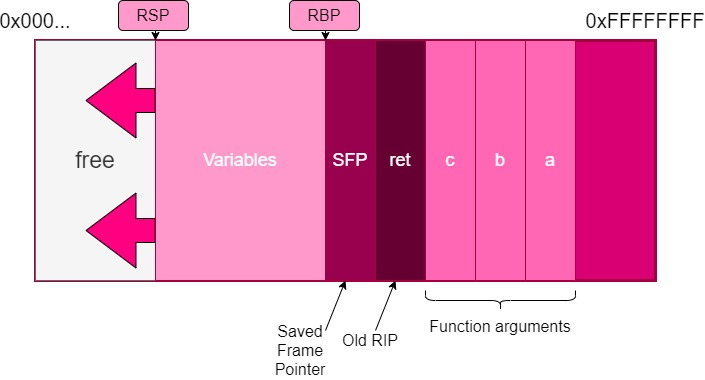
\includegraphics[width=14cm]{stack.jpg}
	\caption{Stack representation right after the function preamble.}
	\label{fig:stack}
\end{figure}

\begin{enumerate}
\item The function arguments are pushed into the stack. We can see them in the stack of Figure \ref{fig:stack} in reverse order. 
\item The function is called:
\begin{enumerate}
	\item The value of register rip is pushed into the stack, so that it is saved for when the function exists. We can see it on Figure \ref{fig:stack} as 'ret'.
	\item The value of rip changes to point to the first instruction of the called function.
\item We execute what is called as the \textit{function preamble} \cite{8664_params_abi_p18}, which prepares the stack frame for the called function:
\begin{enumerate}
	\item The value of rbp is pushed into the stack, so that we can restore the previous stack frame when the function exits. We can see it on Figure \ref{fig:stack} as the 'saved frame pointer'.
	\item The value of rsp is moved into rbp. Therefore, now rbp points to the end of the previous stack frame.
	\item The value of rsp is usually decremented (since the stack needs to go to lower memory addresses) so that we allocate some space for function variables.
\end{enumerate}
\end{enumerate}
\item The function instructions are executed. The stack may be further modified, but on its end rsp must point to the same address of the beginning. Register rbp always keeps pointing to the end of the stack.
\item We execute what is called the \textit{function epilogue}, which removes the stack frame and restores the original function:
\begin{enumerate}
	\item The value of rbp is moved into rsp, so that rsp points to the start of the previous stack frame. All data allocated in the previous stack frame is considered to be free.
	\item The value of the saved frame pointer is popped and stored into rbp, so that rbp now points to the start of the previous stack frame.
	\item The value of the saved rip value is popped into register rip, so that the next instruction to execute is the instruction right after the function call.
\end{enumerate}
\item Since the function arguments where pushed into the stack, they are popped now.
\end{enumerate}


\section{Attacks at the stack} \label{section:attacks_stack}
In Section \ref{subsection:stack}, we studied how the stack works and which is the process that a program follows in order to call a function. As we saw in Figure \ref{fig:stack}, the processor pushes into the stack several data which is used to restore the context of the original function once the called function exits. These pushed arguments included:
\begin{itemize}
\item The arguments with which the function is being called (if they need to be passed in the stack, such as byte arrays).
\item The original value of the rip register (ret), to restore the execution on the original function.
\item The original value of the rbp register (sfp), to restore the frame pointer of the original stack frame.
\end{itemize}

Although this process is simple enough, it opens the possibility for an attacker to easily hijack the flow of execution if it can modify the value of ret, as it is shown in figure \ref{fig:stack_ret_hij_simple}.
\begin{figure}[htbp]
	\centering
	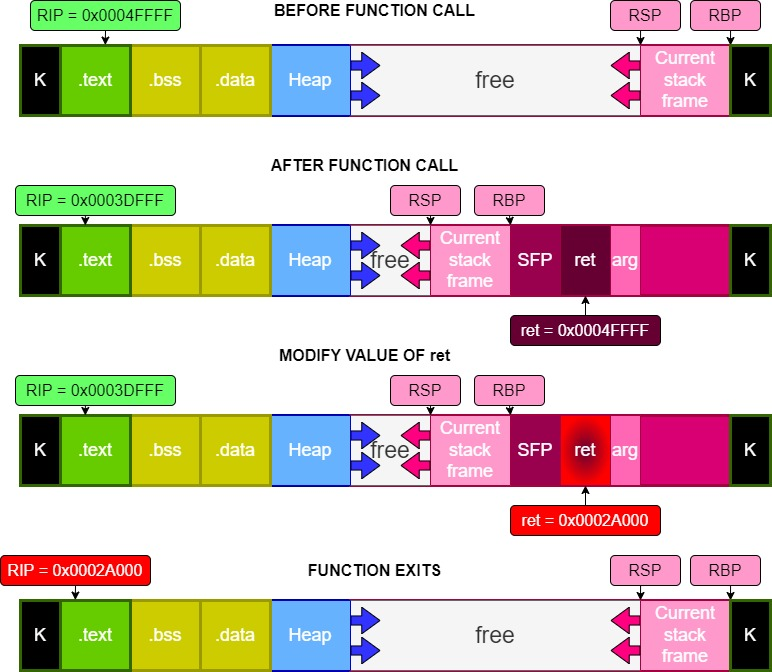
\includegraphics[width=15cm]{stack_ret_hij_simple.jpg}
	\caption{Execution hijack overwriting saved rip value.}
	\label{fig:stack_ret_hij_simple}
\end{figure}

In the Figure, we can observe how, during the execution of the called function, the attacker overwrites the value of ret in the stack. Once the function exists, as we explained in Section \ref{subsection:stack}, during the function epilogue the value of ret will be popped and moved into rip, so that the execution is directed to the original next instruction. However, because the value was modified, the attacker controls which instructions are executed next.

Attackers have historically used multiple techniques to overwrite the ret value in the stack. In this section, we will present two of the most popular techniques, which will be used as a basis for designing our own attacks using eBPF.

\subsection{Buffer overflow} \label{subsection: buf_overflow}
The stack buffer overflow is one of the most popular exploitation techniques to overwrite data at the stack. In this technique, an attacker takes advantage of a program receiving a user value stored in a buffer whose capacity is smaller of that of the supplied value. Code Snippet \ref{code:vuln_overflow} shows an example of a vulnerable program:

\begin{lstlisting}[language=C, caption={Program vulnerable to buffer overflow.}, label={code:vuln_overflow}]
void foo(char *bar){ // bar may be larger than 12 characters
   char buffer[12];
   strcpy(buffer, bar); //no bounds checking 
}

int main(int argc, char *argv[]){
   foo(argv[1]);
   return 0;
}
\end{lstlisting}

During the execution of the above program, since the char array \textit{buffer} is a buffer of length 12 stored in the stack, then if the value of \textit{bar} is larger than 12 bytes it will overflow the allocated space in the stack. This is usually the case of using unsafe functions for processing user input such as strcpy(), which do not check whether the array fits in the buffer. Figure \ref{fig:buffer_overflow} shows how the overflow happens in the stack.

\begin{figure}[htbp]
	\centering
	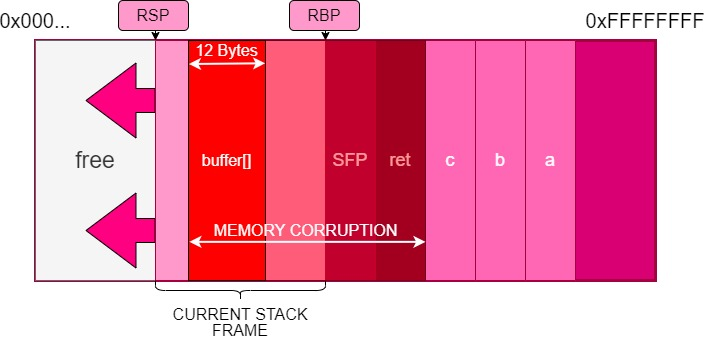
\includegraphics[width=15cm]{buffer_overflow.jpg}
	\caption{Stack buffer overflow overwriting ret value.}
	\label{fig:buffer_overflow}
\end{figure}

As we can observe in the figure, the new data written into the buffer has also overwritten other fields which were pushed into the stack, such as sfp and ret, resulting in changing the flow of execution once the function exists.

Usually, an attacker exploiting a program vulnerable to stack buffer overflow is interested in running arbitrary (malicious) code. For this, the attacker follows the process shown in Figure \ref{fig:buffer_overflow_shellcode}:

\begin{figure}[htbp]
	\centering
	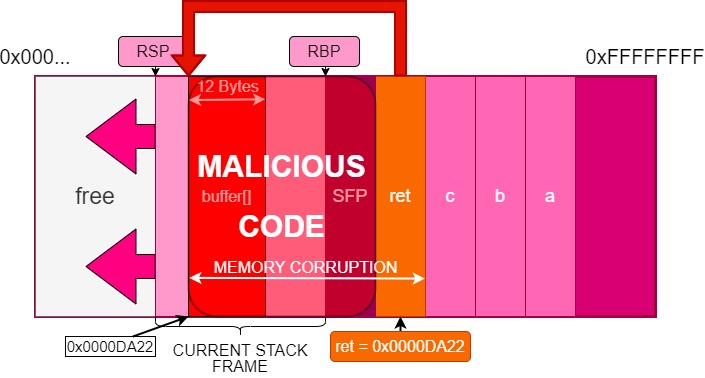
\includegraphics[width=15cm]{buffer_overflow_shellcode.jpg}
	\caption{Executing arbitrary code exploiting a buffer overflow vulnerability.}
	\label{fig:buffer_overflow_shellcode}
\end{figure}

As we can observe in the figure, the attacker will take advantage of the buffer overflow to overwrite not only ret, but also the rest of the current stack frame and sfp with malicious code. This code is known as shellcode, consisting of instruction opcodes (machine assembly instructions translated to their representation in hexadecimal values) which the processor will execute. We will explain how to write shellcode in Section \ref{subsection:got_attack}. Therefore, in this technique the attacker will:
\begin{itemize}
\item Introduce a byte array that overflows the buffer, consisting on SHELLCODE + the address of the buffer.
\begin{itemize}
	\item The shellcode overwrites the buffer and all data until ret.
	\item ret is overwritten by the value of the address where the buffer starts.
\end{itemize}
\item When the function exits and ret is popped from the stack, the register rip will now point to the address of the buffer at the stack, processing the stack data as instructions part of a program. The malicious code will be executed.
\end{itemize}

Although the classic buffer overflow is one of the best-known techniques in binary exploitation, it is also one of the oldest and thus numerous protections have historically been incorporated to mitigate this type of exploits. This is why the attack presented here does not work work in a modern system anymore. 

The reason is that one of the protections consists of the prohibition of executing code from the stack. By marking the stack as non-executable, in the case of rip pointing to an address in the stack any malicious code will not be run, even if an application was vulnerable to a buffer overflow. We will explain more in detail the main protections that nowadays are incorporated in modern systems in Section \ref{subsection:hardening_elf}.

\subsection{Return oriented programming attacks} \label{subsection:rop}
After the stack was marked non-executable, a new refined technique was invented to circumvent this restriction and adapt the classic buffer overflow to modern systems. In the end, attackers still maintained the ability to overflow the buffer in the stack of vulnerable applications, writing shellcode and overwriting ret, the only issue was that the shellcode could not be executed.

Return Oriented Programming (ROP) is an exploitation technique that takes advantage of the fact that, even if malicious code in the stack cannot be executed, the attacker can still redirect the flow of execution by modifying ret to any other piece of executable code. The challenge for the attacker is executing malicious code, since any available executable instructions are either at the .text section (which will correspond to the normal functioning of the program) or at shared libraries, but none are useful for malware. 

ROP tackles this challenge by designing a method of reconstructing malicious code from parts of already-existing code, as in a 'collage'. Assembly instructions are selected from multiple places, so that, when put together and executed sequentially, they recreate the shellcode which the attacker wants to execute. These pieces of code are called ROP gadgets, and consist of a set of arbitrary instructions followed by a final \textit{ret} instruction, which triggers the function exit and pops the value of ret. These gadgets may belong to any code in the process memory, usually selected between the code of the shared libraries (see Figure \ref{fig:stack}) to which the process is linked.

Finding ROP gadgets and writing ROP-compatible payloads manually is hard, thus multiple programs exist that automatically scan the system libraries and construct provide the gadgets given the shellcode to execute \cite{rop_prog_finder}.

However, we will now illustrate how ROP works with an example. Suppose that an attacker has discovered a buffer overflow vulnerability, but the stack is marked as not executable. The attacker wants to execute the assembly code shown in Code Snippet \ref{code:rop_ex}:

\begin{lstlisting}[language=C, caption={Sample program to run using ROP.}, label={code:rop_ex}]
mov rdx, 10
mov rax, [rsp]
\end{lstlisting}

After finding the address of the ROP gadgets manually or using an automated tool, the attacker takes advantage of a buffer overflow (or, in our case, a direct write using eBPF's bpf\_probe\_write\_user()) to overwrite the value of ret with the address of the first ROP gadget, and also additional data in the stack. Figure \ref{fig:rop_compund} shows how we can execute the original program using ROP:

\begin{figure}[htbp]
	\centering
	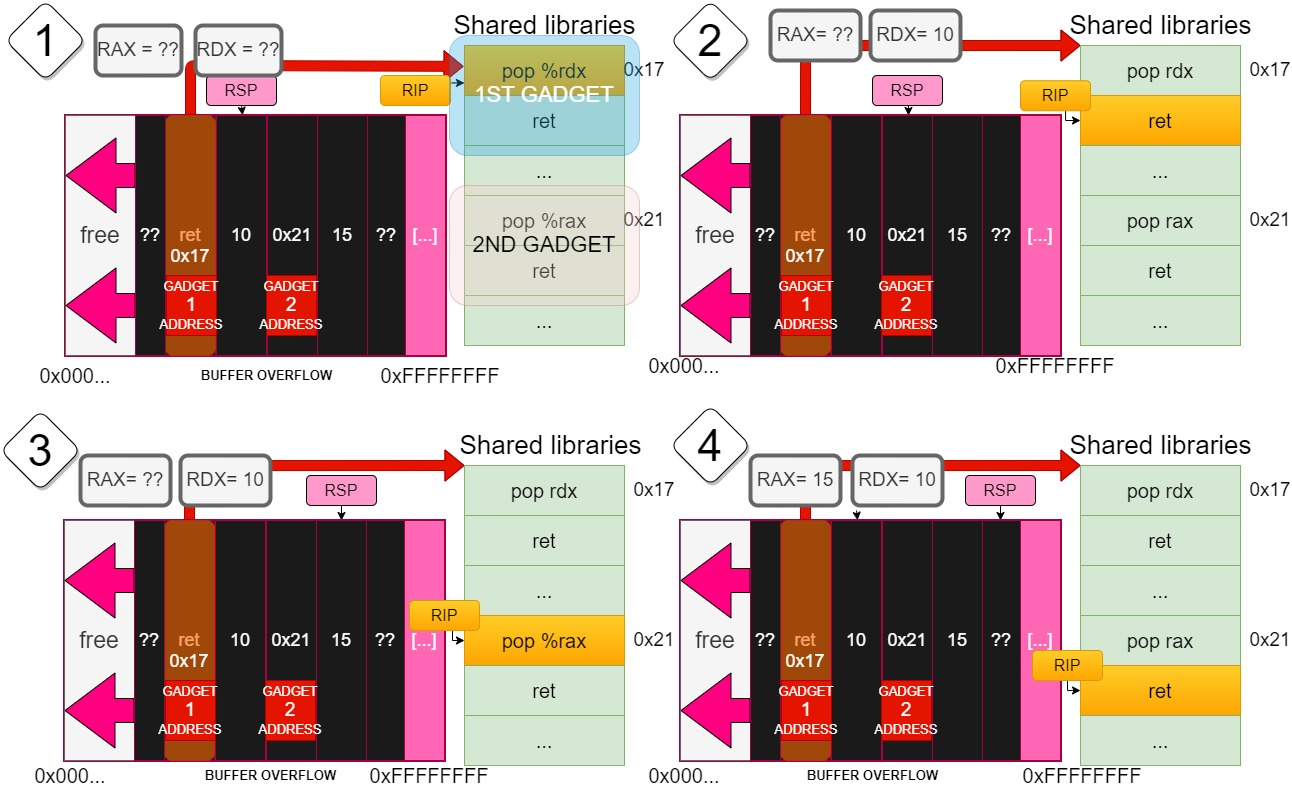
\includegraphics[width=15cm]{ROPcompound.jpg}
	\caption{Steps for executing code sample using ROP.}
	\label{fig:rop_compund}
\end{figure}

The steps described in the figure are the following:
\begin{enumerate}
\item First step shows the two gadgets located and their addresses, and the overwritten data in the stack. The function has already exited and, because ret was overwritten with the address of the first gadget, register rip now points to that location, and thus it is the next instruction to execute. Register rsp, in turn, now points to the bottom address of the current stack frame, which is right next to the old ret (see Section \ref{subsection:stack} for stack frames functioning).
\item The first instruction of the gadget is executed, popping the value from the stack (which also moves register rsp, see stack push and pop operations in Section \ref{subsection:stack}). As we can observe, the value "10" was specifically put in that position by the attacker, so that, according to the instruction to execute \lstinline{mov rdx, 10} \lstinline{}, we now have loaded that data into register rdx.
\item The return instruction is executed, which pops from the stack what is supposed to be the value of the saved rip, but in turn the attacker has placed the address of the next gadget there. Now, rip has jumped to the address of the second gadget. By continuing with this process, we can chain an infinite number of gadgets.
\item Finally, we repeated the same process as before, using a pop instruction to load a value from the stack. This illustrates that push and pop instructions, commonly used on most programs, are also possible to be using ROP.

After this step, the return instruction will be executed. Note that, at this point, if the attacker wants to be stealthy and avoid crashing the program (since we overwrote the original data in the stack), the original stack must be restored, together with the value of the registers before the malicious code execution. We will see an example of a technique for reconstructing the original state during our explanation of the library injection in Section \ref{subsection:got_attack}.
\end{enumerate}



\section{Networking fundamentals in Linux} \label{section:networking_fundamentals}
This section presents an overview on the most relevant aspects of the network system in Linux, which will be needed to tackle multiple of the techniques discussed during the design of the network capabilities of our rootkit. In particular, we will be focusing on the Ethernet, IP and TCP protocols.

\subsection{An overview on the network layer}
Firstly, we will describe the data structure we will be dealing with in networking programs. This will be Ethernet frames containing TCP/IP packets. Figure \ref{fig:frame} shows the frame in its completeness:

\begin{figure}[htbp]
	\centering
	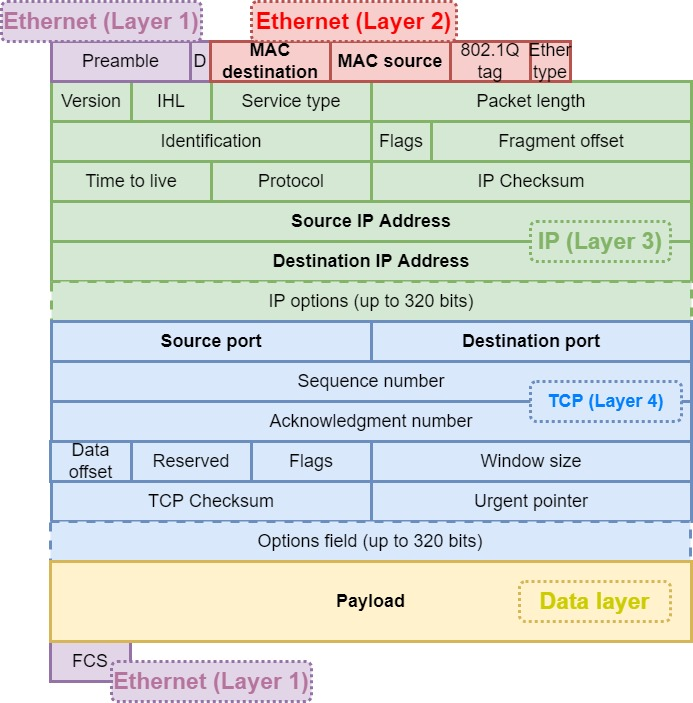
\includegraphics[width=14cm]{frame.jpg}
	\caption{Ethernet frame with TCP/IP packet.}
	\label{fig:frame}
\end{figure}

As we can observe, we can distinguish five different network layers in the frame. This division is made according to the OSI model \cite{network_layers}:
\begin{itemize}
\item Layer 1 corresponds to the physical layer, and it is processed by the NIC hardware, even before it reaches the XDP module (see Figure \ref{fig:xdp_diag}). Therefore, this layer is discarded and completely invisible to the kernel. Note that it does not only include a header, but also a trailer (a Frame Check Sequence, a redundancy check included to check frame integrity).
\item Layer 2 is the data layer, it is in charge of transporting the frame via physical media, in our case an Ethernet connection. Most relevant fields are the MAC destination and source, used for physical addressing.
\item Layer 3 is the network layer, in charge of packet forwarding and routing. In our case, packets will be using the IP protocol. Most relevant fields are the source and destination IP, used to indicate the host that sent the packet and who is the receiver.
\item Layer 4 is the transport layer, in charge of providing end-to-end connection services to applications in a host. We will be focusing on TCP during our research. Relevant fields include the source and destination port, which indicate the ports involved in the communication on which the applications on each host are listening and sending packets.
\item The last layer is the payload of the TCP packet, which contains, according to the OSI model, all layers belong to application data.
\end{itemize}


\subsection{Introduction to the TCP protocol} \label{subsection:tcp}
We will now focus our view on the transport layer, specifically on the TCP protocol, since it will be a major concern at the time of designing the network capabilities of our rootkit.

Firstly, since TCP aims to offer a reliable and ordered packet transmission \cite{tcp_reliable}, it includes sequence numbers (see Table \ref{fig:frame}) which mark the order in which they are transmitted. However, since the physical medium may corrupt or lose packets during the transmission, TCP must incorporate mechanisms for ensuring the order and delivery of all packets:
\begin{itemize}
\item Mechanism for opening and establishing a reliable connection between two parties.
\item Mechanism for ensuring that packets are retransmitted in case of an error during the connection.
\end{itemize}

With respect to the establishment of a reliable connection, this is achieved via a 3-way handshake, in which certain TCP flags will be set in a series of interchanged packets (see in Figure \ref{fig:frame} the field TCP flags). Most relevant TCP flags are described in Table \ref{table:tcp_flags}.

\begin{table}[htbp]
\begin{tabular}{|>{\centering\arraybackslash}p{3cm}|>{\centering\arraybackslash}p{10cm}|}
\hline
\textbf{FLAG} & \textbf{PURPOSE}\\
\hline
\hline
ACK & Acknowledges that a packet has been successfully received. In the acknowledgment number (see figure \ref{fig:frame}), it is stored the sequence number of the packet being acknowledged + 1. \\
\hline
SYN & Used during the 3-way handshake, indicates request for establishing a connection.\\
\hline
FIN & Used to request a connection termination.\\
\hline
RST & Abruptly terminates the connection, usually sent when a host receives an unexpected or unrecognized packet.\\
\hline
\end{tabular}
\caption{Relevant TCP flags and their purpose.}
\label{table:tcp_flags}
\end{table}

Taking the above into account, Figure \ref{fig:tcp_conn} shows a depiction of the 3-way handshake \cite{tcp_handshake}:
\begin{figure}[htbp]
	\centering
	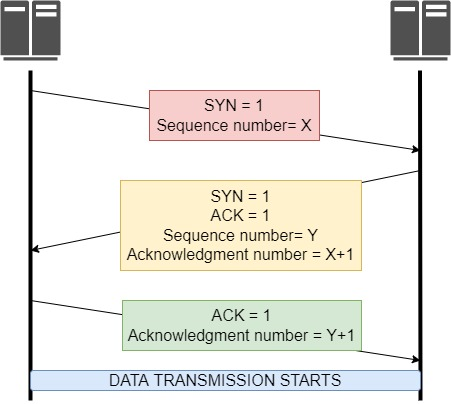
\includegraphics[width=12cm]{tcp_conn.jpg}
	\caption{TCP 3-way handshake.}
	\label{fig:tcp_conn}
\end{figure}

As we can observe in the figure, the hosts interchange a sequence of SYN, SYN+ACK, ACK packets, after which the communication starts. During this communication, the sender transmits packets with data (and no flags set), to which it expects an ACK packet acknowledging having received it.

With respect to maintaining the integrity of the connection once it starts, TCP works using timers, as it is illustrated in Figure \ref{fig:tcp_retransmission}:
\begin{enumerate}
\item A data packet with sequence number X is sent. The timer starts.
\item The destination host receives the packet and returns an ACK packet with acknowledgment number X+1.
\item The sender receives the ACK packet and stops the timer. If, for any reason, the ACK packet is not received before the timer ends, then the same packet is retransmitted.
\end{enumerate}

\begin{figure}[htbp]
	\centering
	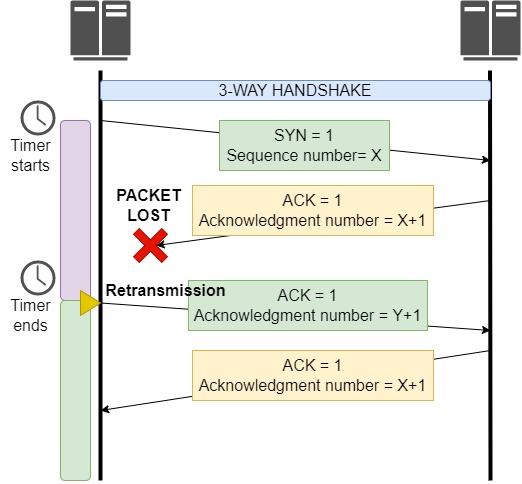
\includegraphics[width=12cm]{tcp_retransmission.jpg}
	\caption{TCP packet retransmission on timeout.}
	\label{fig:tcp_retransmission}
\end{figure}

\section{ELF binaries} \label{section:elf}
This section details the Executable and Linkable Format (ELF) \cite{elf}, the format in which we find executable files (between other file types) in Linux systems. We will perform an analysis from a security standpoint, that is, mainly oriented to describe the most relevant sections and the permissions incorporated into them. We will also focus on several of these sections which will be relevant for designing our attack.

After that, we will overview the security hardening techniques that have been historically incorporated into Linux to mitigate possible exploitation techniques when running ELF executables (such as the stack buffer overflow we explained in Section \ref{subsection: buf_overflow}). During the design of our rootkit, we will attempt to bypass these techniques using multiple workarounds.

\subsection{The ELF format and Lazy Binding} \label{subsection:elf_lazy_binding}
Linux supports multiple tools that enable a deep inspection of ELF binaries and its sections. Table \ref{table:elf_tools} shows the main tools we will use during this analysis:

\begin{table}[htbp]
\begin{tabular}{|>{\centering\arraybackslash}p{3cm}|>{\centering\arraybackslash}p{10cm}|}
\hline
\textbf{TOOL} & \textbf{PURPOSE}\\
\hline
\hline
Readelf & Display information about ELF files\\
\hline
Objdump & Display information about object files, mainly used for decompiling programs\\
\hline
GDB & The GNU Project Debugger, allows for debugging programs during runtime\\
\hline
GDB-peda & The Python Exploit Development Assistance for GDB, allows for multiple advanced operations that ease exploit development, such as showing register values, the stack state or memory information. It works as a plugin for GDB.\\
\hline
\end{tabular}
\caption{Tools used for analysis of ELF programs.}
\label{table:elf_tools}
\end{table}

Firstly, we will analyse the main sections we can find in an ELF executable. We will approach this study using a sample program that has been compiled using Clang/LLVM, and that consists on a simple timer that counts twice up to number 3, available at our repository \cite{repo_simple_timer}.

The commands used for this analysis and complete list of headers can be found in \nameref{annex:readelf_commands}. The most relevant sections we found at the program are described in Table \ref{table:elf_sec_headers}:

\begin{table}[htbp]
\begin{tabular}{|>{\centering\arraybackslash}p{1cm}|>{\centering\arraybackslash}p{9cm}|>{\centering\arraybackslash}p{2cm}|}
\hline
\textbf{TOOL} & \textbf{PURPOSE} & \textbf{PERMS}\\
\hline
\hline
.init & Contains instructions executed before the \textit{main} function of the program & Alloc, Executable\\
\hline
.plt & Procedure Linkage Table (PLT), contains code stubs that use the addresses at .got.plt for jumping to position-independent code & Alloc, Executable\\
\hline
.got & Global Offset Table (GOT), it contains addresses of global variables and functions once the linker resolves them at runtime & Alloc, Writable\\
\hline
.got.plt & A subset of .got section separated from .got with some compilers, it contains only the target addresses of position-independent code once the linker loads them at runtime, used by .plt section. & Alloc, Writable\\
\hline
.plt.got & Generated depending on compiler options, it is a PLT section which does not use lazy binding. & Alloc, Executable\\
\hline
.text & Stores executable instructions. & Alloc, Executable\\
\hline
.data & Contains initialized static and global variables. & Alloc, Writable\\
\hline
.bss & Contains global and static variables which are uninitialized or initialized to zero. & Alloc, Writable\\
\hline 
\end{tabular}
\caption{Sections in an ELF file.}
\label{table:elf_sec_headers}
\end{table}

As it can be observed in Table \ref{table:elf_sec_headers}, we can find that all sections have the Alloc flag, meaning they will be loaded into process memory during runtime.

Apart from those we have already discussed previously, we can find the GOT and PLT sections, whose purpose is to support Position Independent Code (PIC), that is, instructions whose address in virtual memory is not hardcoded by the compiler into the executable, but rather they are not known until resolved at runtime. This is usually the case of shared libraries, which can be loaded into virtual memory starting at any address \cite{plt_got_overlord}.

Therefore, in order to call a function of a shared library, the dynamic linker follows a process called 'Lazy binding' \cite{plt_got_technovelty}:
\begin{enumerate}
\item From the .text section, instead of calling a direct absolute address as usual, a PLT stub (in the .plt section) is called. Snippet \ref{code:lazy_bind_1} shows a call to the function timerfd\_settime, implemented by the shared library glibc and thus using a PLT.
\begin{lstlisting}[language=C, caption={Call to PLT stub seen from objdump.}, label={code:lazy_bind_1}]
$ objdump -d simple_timer
4014cb:	b9 00 00 00 00       	mov    $0x0,%ecx
4014d0:	be 01 00 00 00       	mov    $0x1,%esi
4014d5:	89 c7                	mov    %eax,%edi
4014d7:	e8 44 fc ff ff       	call   401120 <timerfd_settime@plt>
\end{lstlisting}

\item In the PLT stub, the flow of execution jumps to an address which is stored in the GOT section, which is the absolute address of the function at glibc. This address must be written there by the dynamic linker but, according to lazy binding, the first time to call this function the linker has not calculated that address yet. 

\begin{figure}[htbp]
	\centering
	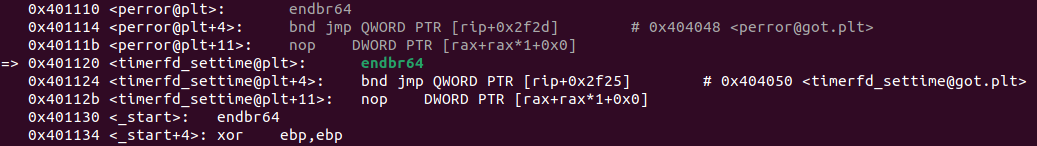
\includegraphics[width=14.5cm]{sch_gdb_plt.png}
	\caption{PLT stub for timerfd\_settime, seen from gdb-peda.}
	\label{fig:lazy_bind_2}
\end{figure}

\begin{figure}[htbp]
	\centering
	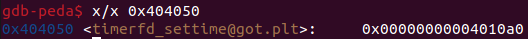
\includegraphics[width=14.5cm]{sch_gdb_got_prev.png}
	\caption{Inspecting address stored in GOT section before dynamic linking, seen from gdb-peda.}
	\label{fig:lazy_bind_3}
\end{figure}

\item As we can see in Figures \ref{fig:lazy_bind_2} and \ref{fig:lazy_bind_3}, the PLT stub calls address 0x4010a0, which leads to a dynamic linking routine, which proceeds to write the address into the GOT section and jump back to the start of the PLT stub. This time, the memory address at GOT to which the PLT jumps is already loaded with the address to the function at the shared library, as shown by Figure \ref{fig:lazy_bind_4}.

\begin{figure}[htbp]
	\centering
	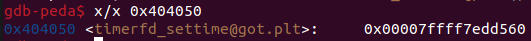
\includegraphics[width=14.5cm]{sch_gdb_got_after.png}
	\caption{Inspecting address stored in GOT section after dynamic linking, seen from gdb-peda.}
	\label{fig:lazy_bind_4}
\end{figure}

\begin{figure}[htbp]
	\centering
	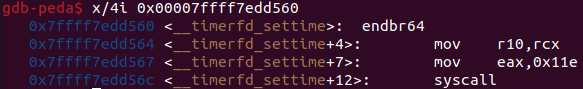
\includegraphics[width=14.5cm]{sch_glibc_func.png}
	\caption{Glibc function to which PLT jumps using address stored at GOT, seen from gdb-peda.}
	\label{fig:lazy_bind_5}
\end{figure}

\end{enumerate}

Therefore, in essence, when using lazy binding the dynamic linker will individually load into GOT the addresses of the functions at the shared libraries, during the first time they are called in the program. After that, the address will remain in the GOT section and will be used by the PLT for all subsequent calls.

The reason lazy binding matters to us is because, as we will explain Section \ref{subsection:got_attack}, the GOT section is actually writable from an eBPF program. This is because this section specifically must be writeable at runtime for the dynamic linker to store the address once they are resolved. Therefore, we would be able to modify the GOT section from eBPF, redirecting the address at which the PLT jumps, and thus controlling the flow of execution in the program. 

\subsection{Hardening ELF binaries} \label{subsection:hardening_elf}
During Section \ref{section:attacks_stack}, we presented multiple of the classic attacks at the stack such as buffer overflow and ROP. However, as we mentioned, during the years multiple hardening measures have been introduced into modern compilers, which attempt to mitigate these and other techniques. We will now present them so that, during the design of our rootkit, we can attempt to bypass all of these.

Table \ref{table:compilers} shows the compilers that we will be considering during this study. We will be exclusively looking at those security features that are included by default.

\begin{table}[htbp]
\begin{tabular}{|>{\centering\arraybackslash}p{5cm}|>{\centering\arraybackslash}p{9cm}|}
\hline
\textbf{COMPILER} & \textbf{SECURITY FEATURES BY DEFAULT}\\
\hline
\hline
Clang/LLVM 12.0.0 (2021) & Stack canaries, DEP/NX, ASLR\\
\hline
GCC 10.3.0 (2021) & Stack canaries, DEP/NX, ASLR, PIE, Full RELRO\\
\hline 
\end{tabular}
\caption{Security features in C compilers used in the study.}
\label{table:compilers}
\end{table}

\textbf{Stack canaries}\\
Stack canaries are random data that is pushed into the stack before calling potentially vulnerable functions (such as strcpy()) that attempts to prevent attacks at the stack by ensuring that their value is the same before and after the execution of the called function. It is particularly useful at detecting buffer overflow attacks.

If a stack canary is present and a buffer overflow happened, it would potentially overwrite the value of the canary, therefore alerting of the attack, in which case the processor halts the execution of the program.

\textbf{DEP/NX}\\
Data Execution Prevention, also known as No Execute, is the option of marking the stack as non-executable. This prevents, as we explained in Section \ref{subsection: buf_overflow}, the possibility of executing injected shellcode in the stack after modifying the value of the saved rip.

The creation of advanced techniques like ROP is one reaction to this mitigation, that circumvents this protection.

\textbf{ASLR}\\
Address Space Layout Randomization is a technique that randomizes the position of memory sections in a process virtual memory, including the heap, stack and libraries, so that an attacker cannot rely on known addresses during exploitation (e.g.: libraries are loaded at a different memory address each time the program is run, so ROP gadgets change their position) \cite{aslr_pie_intro}.

In the context of a stack buffer overflow attack, the memory position of the stack is random, and therefore even if shellcode is injected into the stack by an attacker, the address at which it resides cannot be written into the saved value of rip in order to hijack the flow of execution.

\textbf{PIE}\\
Position Independent Executable is a mitigation introduced to reduce the ability of an attacker to locate symbols in virtual memory by randomizing the base address at which the program itself (including the .text section) is loaded. This base address determines an offset which is added to all memory addresses in the code, so that each instruction is located at an address + this offset. Therefore, all jumps are made using relative addresses \cite{aslr_pie_intro}.

\textbf{RELRO}\\
Relocation Read-Only is a hardening technique that mitigates the possibility of an attacker overwriting the GOT section, as we explained at Section \ref{subsection:elf_lazy_binding}. In order to achieve the lazy binding process is substituted by the linker resolving all entries in the GOT section right after the beginning of the execution, and then marking the .got section as read-only. 

Two settings for RELRO are the most widespread, either Partial RELRO (which only marks sections of the .got section not related to the PLT as read-only, leaving .got.plt writeable) or Full RELRO (which marks the .got section as read-only completely). Binaries with only Partial RELRO are still non-secure, as the address at which the PLT section jumps can still be overwriten (including from eBPF, as we will explain) \cite{relro_redhat}.

\textbf{Intel CET}\\
Intel Control-flow Enforcement Technology is a hardening feature fully incorporated in Windows 10 systems \cite{cet_windows} and a work in progress in Linux \cite{cet_linux}. Its purpose is to defeat ROP attacks and other derivates (e.g: Jump-oriented programming, JOP), by adding a strict kernel-supported control of the return addresses and strong restrictions over jump and call instructions.

In Linux, the kernel will support a hidden 'shadow stack' that will save the return addresses for each call. This prevents modifying the saved value of rip in the stack, since the kernel would realise that the flow of execution has been modified. We can also find that modern compilers (such as GCC 10.3.0) already generate Intel CET-related instructions such as \textit{endbr64}, whose purpose is to be placed at the start of functions, marking that as the only address to which an indirect jump can land (otherwise, jumps will be rejected if not landing at \textit{endbr64}).

As mentioned, we will not consider this feature since it is not active in the Linux kernel.

\section{The proc filesystem} \label{section:proc_filesystem}
The proc filesystem is a virtual filesystem which provides an interface to kernel data structures \cite{proc_fs}. It can be found mounted automatically at \textit{/proc}.

This filesystem offers a great range of capabilities to interact with the kernel internal structures, however, in this section, we will focus on the most relevant files and directories for our research.

Specifically, we will be studying the files under the \textit{/proc/<pid>/} directory, whose purpose is to expose information about the process with the corresponding process ID.

Note that the access control for the \textit{/proc/<pid>/} is governed by the value set at \textit{/proc/sys/kernel/yama/ptrace\_scope}. Table \ref{table:yama_values} show its possible values.

\begin{table}[htbp]
\begin{tabular}{|>{\centering\arraybackslash}p{3cm}|>{\centering\arraybackslash}p{11cm}|}
\hline
\textbf{VALUE} & \textbf{DESCRIPTION}\\
\hline
\hline
0 & Unprivileged processes may access any file or subdirectory\\
\hline
1 & Only privileged processes or those belonging to that PID may access the any file. Unprivileged process can still list the directories at \textit{/proc}, finding the complete list of running processes.\\
\hline
2 & Only privileged processes or those belonging to that PID may access the any file. Unlike with setting '1', unprivileged users cannot list the directores at \textit{/proc} anymore.\\ 
\hline
\end{tabular}
\caption{Values for \textit{/proc/sys/kernel/yama/ptrace\_scope}.}
\label{table:yama_values}
\end{table}

In Ubuntu 21.04, the value of this setting is of '1', therefore the access is limited to users with root privileges or to unprivileged users accessing only their own or their children process information.

\subsection{/proc/<pid>/maps} \label{subsection:proc_maps}
This file provides, for the process with process ID <pid>, its mapped memory regions and their access permissions, that is, those virtual memory pages actively connected to a physical memory page (as shown in Figure \ref{fig:mem_arch_pages}).

Figure \ref{fig:proc_maps_sample} shows the maps file of a simple program. As we can observe, by reading this file we can get information such as:
\begin{itemize}
\item The virtual addresses that limit each memory section.
\item The permissions over each memory section.
\item In the case of memory from a file, the offset from which the data was loaded.
\item A pathname, in the case that memory section was loaded from a file.

The ability to easily find memory sections on the virtual address space of a process with a specific set of permissions is particularly relevant for this research. Also, apart from disclosing the address of the stack (and sometimes the heap too), we can infer the address of other memory sections such as the .text section, which must be the only one marked as executable (in Figure \ref{fig:proc_maps_sample}, the second entry that appears).

\end{itemize}

\begin{figure}[htbp]
	\centering
	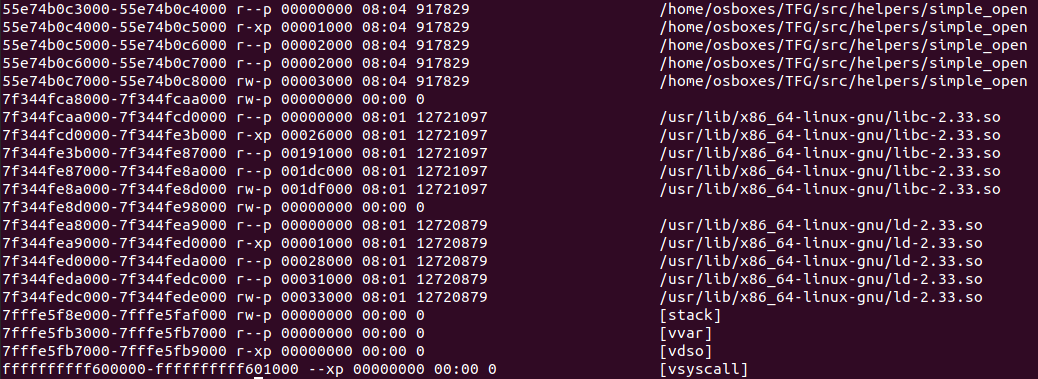
\includegraphics[width=15cm]{sch_proc_maps_sample.png}
	\caption{File /proc/<pid>/maps of a sample program.}
	\label{fig:proc_maps_sample}
\end{figure}

\subsection{/proc/<pid>/mem}
This file enables a process to access the virtual memory of the process with process id <pid>. According to the documentation, "this file can be used to access the pages of a process's memory through open(2), read(2), and lseek(2)" \cite{proc_fs}, meaning that we can read any memory address from the virtual memory space of the process.

However, we found the documentation not to be complete. In our experience, not only we can read virtual memory, but also freely write into it. There existed some discussions in the Linux community, and it was considered safe enough to be set as writeable by privileged programs \cite{proc_mem_write}, although the changes were never reflected in the official documentation.

Apart from being able to write into virtual memory, this write accesses are performed without regard of the permission flags set on each memory section. Therefore, we can modify non-writeable virtual memory by writing into the \textit{/proc/<pid>/mem} file.


\chapter{Analysis of offensive capabilities} \label{chapter:analysis_offensive_capabilities}
In the previous chapter, we detailed which functionalities eBPF offers and studied its underlying architecture. As with every technology, a prior deep understanding is fundamental for discussing its security implications. 

Therefore, given the previous background, this chapter is dedicated to an analysis in detail of the security implications of a malicious use of eBPF. For this, we will firstly explore the security features incorporated in the eBPF system. Then, we will identify the fundamental pillars onto which malware can build their functionality. As we mentioned during the project goals, these main topics of research will be the following:
\begin{itemize}
\item Analysing eBPF's possibilities when hooking system calls and kernel functions.
\item Learning eBPF's potential to read/write arbitrary memory.
\item Exploring networking capabilities with eBPF packet filters.
\end{itemize}


%TODO if this is finally not included, change the intro
Finally, we will study in detail some of the malicious applications that previous researchers have proposed to take advantage of these capabilities of eBPF. In the next chapter, we will proceed to elaborate on these ideas, find new purposes and design our own rootkit.


\section{eBPF maps security}
In table \ref{table:ebpf_caps_current}, we observed that only programs with CAP\_SYS\_ADMIN are allowed to iterate over eBPF maps. The reason why this is restricted to privileged programs is because it is functionality that is a potential security vulnerability, which we will now proceed to analyse.

In subsection \ref{subsection:ebpf_maps} we mentioned that eBPF maps are opened by specifying an ID (which works similarly to the typical file descriptors), while in table \ref{table:ebpf_map_types} we showed that, for performing operations over eBPF maps using the bpf() syscall, the map ID must be specified too. 

Map IDs are known by a program after creating the eBPF map, however, a program can also explore all the available maps in the system by using the BPF\_MAP\_GET\_NEXT\_ID operation in the bpf() syscall, which allows for iterating through a complete hidden list of all the maps created. This means that privileged programs can find and have read and write access to any eBPF map used by any program in the system.

Therefore, a malicious privileged eBPF program can access and modify other programs' maps, which can lead to:
\begin{itemize}
\item Modify data used for the program operation. This is the case for maps which mainly store data structures, such as BPF\_MAP\_TYPE\_HASH.
\item Modify the program control flow, altering the instructions executed by an eBPF program. This can be achieved if a program is using the bpf\_tail\_call() helper (introduced in table \ref{table:ebpf_helpers}) which is taking data from a map storing eBPF programs (BPF\_MAP\_TYPE\_PROG\_ARRAY, introduced in table \ref{table:ebpf_map_types}).
\end{itemize}


\section{Abusing tracing programs}
eBPF tracing programs (kprobes, uprobes and tracepoints) are hooked to specific points in the kernel or in the user space, and call probe functions once the flow of execution reaches the instruction to which they are attached. This section details the main security concerns regarding this type of programs.

\subsection{Access to function arguments}
As we saw in section \ref{section:ebpf_prog_types}, tracing programs receive as a parameter those arguments with which the hooked function originally was called. These parameters are read-only and thus, in principle, they cannot be modified inside the tracing program (we will show this is not entirely true in section \ref{section:mem_corruption}). The next code snippets show the format in which parameters are received when using libbpf (Note that libbpf also includes  some macros that offer an alternative format, but the parameters are the same).


\begin{lstlisting}[language=C, caption={Probe function for a kprobe on the kernel function vfs\_write.}, label={code:format_kprobe}]
SEC("kprobe/vfs_write")
int kprobe_vfs_write(struct pt_regs* ctx){
\end{lstlisting}

\begin{lstlisting}[language=C, caption={Probe function for an uprobe, execute\_command is defined from user space.}, label={code:format_uprobe}]
SEC("uprobe/execute_command")
int uprobe_execute_command(struct pt_regs *ctx){
\end{lstlisting}

\begin{lstlisting}[language=C, caption={Probe function for a tracepoint on the start of the syscall sys\_read.}, label={code:format_tracepoint}]
SEC("tp/syscalls/sys_enter_read") 
int tp_sys_enter_read(struct sys_read_enter_ctx *ctx) { 
\end{lstlisting}

In code snippets \ref{code:format_kprobe} and \ref{code:format_uprobe} we can identify that the parameters are passed to kprobe and uprobe programs as a pointer to a \textit{struct pt\_regs*}. This struct contains as many attributes as registers exist in the system architecture, in our case x86\_64. Therefore, on each probe function, we will receive the state of the registers at the original hooked function. This explains the format of the \textit{struct pt\_regs}, shown in code snippet \ref{code:format_ptregs}:

\begin{lstlisting}[language=C, caption={Format of struct pt\_regs.}, label={code:format_ptregs}]
struct pt_regs {
	long unsigned int r15;
	long unsigned int r14;
	long unsigned int r13;
	long unsigned int r12;
	long unsigned int bp;
	long unsigned int bx;
	long unsigned int r11;
	long unsigned int r10;
	long unsigned int r9;
	long unsigned int r8;
	long unsigned int ax;
	long unsigned int cx;
	long unsigned int dx;
	long unsigned int si;
	long unsigned int di;
	long unsigned int orig_ax;
	long unsigned int ip;
	long unsigned int cs;
	long unsigned int flags;
	long unsigned int sp;
	long unsigned int ss;
};
\end{lstlisting}

By observing the value of the registers, we are able to extract the parameters of the original hooked function. This can be done by using the System V AMD64 ABI\cite{8664_params_abi}, the calling convention used in Linux. Depending on whether we are in the kernel or in user space, the registers used to store the values of the function arguments are different. Table \ref{table:systemv_abi} summarizes these two interfaces. 

\begin{table}[H]
\begin{tabular}{|>{\centering\arraybackslash}p{2cm}|>{\centering\arraybackslash}p{3cm}|}
\hline
\multicolumn{2}{|c|}{User interface}\\
\hline
Register & Purpose\\
\hline
\hline
rdi & 1st argument\\
\hline
rsi & 2nd argument\\
\hline
rdx & 3rd argument\\
\hline
rcx & 4th argument\\
\hline
r8 & 5th argument\\
\hline
r9 & 6th argument\\
\hline
rax & Return value\\
\hline
\end{tabular}
\quad
\begin{tabular}{|>{\centering\arraybackslash}p{2cm}|>{\centering\arraybackslash}p{3cm}|}
\hline
\multicolumn{2}{|c|}{Kernel interface}\\
\hline
Register & Purpose\\
\hline
\hline
rdi & 1st argument\\
\hline
rsi & 2nd argument\\
\hline
rdx & 3rd argument\\
\hline
r10 & 4th argument\\
\hline
r8 & 5th argument\\
\hline
r9 & 6th argument\\
\hline
rax & Return value\\
\hline
\end{tabular}
\caption{Argument passing convention of registers for function calls in user and kernel space respectively.}
\label{table:systemv_abi}
\end{table}

In the case of tracepoints, we can see in code snippet \ref{code:format_tracepoint} that it receives a \textit{struct sys\_read\_enter\_ctx*}. This struct must be manually defined, as explained in \ref{subsection:tracepoints}, by looking at the file \textit{/sys/kernel/debug/tracing/events/syscalls/sys\_enter\_read/format}. Code snippet \ref{code:sys_enter_read_tp} shows the format of the struct.

\begin{lstlisting}[language=C, caption={Format for parameters in sys\_enter\_read specified at the format file.}, label={code:sys_enter_read_tp_format}]
field:unsigned short common_type; offset:0; size:2; signed:0;
field:unsigned char common_flags; offset:2; size:1; signed:0;
field:unsigned char common_preempt_count; offset:3; size:1; signed:0;
field:int common_pid; offset:4; size:4; signed:1;
field:int __syscall_nr;	offset:8; size:4; signed:1;
field:unsigned int fd; offset:16; size:8; signed:0;
field:char * buf; offset:24; size:8; signed:0;
field:size_t count; offset:32; size:8; signed:0;
\end{lstlisting}

\begin{lstlisting}[language=C, caption={Format of custom struct sys\_read\_enter\_ctx.}, label={code:sys_enter_read_tp}]
struct sys_read_enter_ctx {
    unsigned long long pt_regs;
    int __syscall_nr;
    unsigned int padding;
    unsigned long fd;
    char* buf;
    size_t count;
};
\end{lstlisting}

As we can observe, we are given a set of attributes which include the parameters with which the syscall was called. Moreover, we can still obtain an address pointing to another \textit{struct pt\_regs}, as in kprobes and uprobes, by combining the first four fields and considering it as a 32-bit long address. This means we will still be able to extract the value of the rest of the registers too. 

It must be noted that, in syscalls, in addition to use the kernel parameter passing convention specified in table \ref{table:systemv_abi}, the number specifying the syscall must be passed in register rax too.

On a final note, as we mentioned in section \ref{section:ebpf_prog_types}, there exist differences in the parameters received in probe functions depending on the two variations of tracing programs. Therefore:
\begin{itemize}
\item kprobe, uprobe and \textit{enter} tracepoints will receive the full parameters as we specified before, but not the return value of the function (since it is not executed yet).
\item kretprobes, uretprobes and \textit{exit} tracepoints will still receive the \textit{struct pt\_regs}, but without any of the parameters and with only the return value of the function.
\end{itemize}

Taking into account all the previous, the fact that tracing programs have read-only access to function arguments can be considered an useful and needed feature for tracing applications, but malicious eBPF can use this for purposes such as:
\begin{itemize}
\item Gather kernel and user data passed to a function as a parameter. In many cases this information can be potentially interesting for an attacker, such as passwords.
\item Store in eBPF maps information about system activities, to be used by other malicious eBPF programs.
\end{itemize}

Usually, since many function arguments are pointers to user or kernel addresses (such as buffers where a string or a struct with data is located), eBPF tracing programs can use two eBPF helpers that enable to read large byte arrays from both kernel and user space:
\begin{itemize}
\item bpf\_probe\_read\_user()
\item bpf\_probe\_read\_kernel()
\end{itemize}

These helpers, previously introduced in table \ref{table:ebpf_helpers}, enable to read an arbitrary number of bytes from an user or kernel address respectively, allowing us to extract the information pointed by the parameters received by eBPF programs.

\subsection{Reading memory out of bounds} \label{subsection:out_read_bounds}
As we introduced in the previous subsection, the bpf\_probe\_read\_user() and bpf\_probe\_read\_kernel() helpers can be used to access memory of pointers received as parameters in the hooked functions. 

However, although in general the eBPF verifier attempts to reject illegal memory accesses, it does not prevent a malicious program from passing an arbitrary memory address (in kernel or user space) to the above helpers. This means that an eBPF program can potentially read any address in user or kernel space, (as long as it is marked as readable in the corresponding memory pages). Furthermore, an attacker can locate specific data structures and memory sections by taking the function parameter as a reference point in memory.

A particularly relevant case (which we will later use for our rootkit) involves accessing user memory via the parameters of tracepoints attached at system calls. Provided the nature of syscalls, whose purpose is to communicate user and kernel space, all parameters received will belong to the user space, and therefore any pointer passed will be an address in user memory. This enables an eBPF program to get a foothold into the virtual address space of the process calling the syscall, which it can proceed to scan looking for data or specific instructions. This technique will be further elaborated in section \ref{subsection_bpf_probe_write_apps}.

\subsection{Overriding function return values}
A potentially dangerous functionality in eBPF tracing programs is the ability to modify the return value of kernel functions\cite{ebpf_friends_p15}\cite{ebpf_override_return}. This can be done via the eBPF helper bpf\_override\_return, and it works exclusively from kretprobes.

Apart from only working on kretprobes, additional restrictions are applied to this helper. It will only work if the kernel was compiled with the CONFIG\_BPF\_KPROBE\_OVERRIDE flag, and only if the kretprobe is attached to a function to which, during the kernel development, the macro ALLOW\_ERROR\_INJECTION() has been indicated. Currently, only a small selection of functions include this macro, but most system calls can be found to implement it. The following code snippets show how a system call like sys\_open is defined in kernel v5.11:

\begin{lstlisting}[language=C, caption={Definition of the syscall sys\_open in the kernel \cite{code_kernel_open}}, label={code:override_return_1}]
SYSCALL_DEFINE3(open, const char __user *, filename, int, flags, umode_t, mode)
{
	if (force_o_largefile())
		flags |= O_LARGEFILE;
	return do_sys_open(AT_FDCWD, filename, flags, mode);
}
\end{lstlisting}

\begin{lstlisting}[language=C, caption={Definition of the macro for creating syscalls, containing the error injection macro. Only relevant instructions included, complete macro can be found in the kernel \cite{code_kernel_syscall}}, label={code:override_return_2}]
#define SYSCALL_DEFINE3(name, ...) SYSCALL_DEFINEx(3, _##name, __VA_ARGS__)
#ifndef __SYSCALL_DEFINEx
#define __SYSCALL_DEFINEx(x, name, ...)\
	[...]
	ALLOW_ERROR_INJECTION(sys##name, ERRNO);\
	[...]
\end{lstlisting}


By looking at snippets \ref{code:override_return_1} and \ref{code:override_return_2}, we can observe that the system call sys\_open involves the inclusion of the ALLOW\_ERROR\_INJECTION macro. Therefore, any kretprobe attached to a system call function will be able to modify its return value.

In order to be able to modify the return value of functions, the aforementioned eBPF helper makes use of the fault injection framework of the Linux kernel\cite{fault_injection}, which was created before eBPF itself, and whose original purpose is to allow for generating errors in kernel programs for debugging purposes.

Taking the previous information into account, we can find that a malicious eBPF program, by tampering with the kernel-user space interface which are system calls, can mislead user programs, which trust the output of kernel code. This can lead to:
\begin{itemize}
\item A program believes a system call exited with an error, while in reality the kernel completed the operation with success, or viceversa. For instance, the result of a call to sys\_open can mislead a user program into thinking that a file does not exist.
\item A program receives incorrect data on purpose. For instance, a buffer may look empty or of a reduced size upon a sys\_read call, while in reality more data is available to be read.
\end{itemize}

\subsection{Sending signals to user programs}
Another eBPF helper that is subject to malicious purposes is bpf\_send\_signal. This helper enables to send an arbitrary signal to the thread of the process running a hooked function.

Therefore, this helper can be used to forcefully terminate running user processes, by sending the SIGKILL signal. In this way, combined with the observability into the parameters received at a function call, malicious eBPF can kill and deactivate processes to favour its malicious purposes.

\subsection{Takeaways} \label{subsection:tracing_attacks_conclusion}
As a summary, a malicious eBPF program loaded and attached as a tracing program undermines the existing trust between user programs and the kernel space. 

Its ability to access sensitive data in function parameters and reading arbitrary memory can lead to gathering extensive information on the running processes of a system, whilst the malicious use of eBPF helpers enables the modification of the data passed to the user space from the kernel, and the control over which programs are allowed to be running on the system.

\section{Memory corruption} \label{section:mem_corruption}
In the previous section we described how tracing programs can read user memory out of the bounds of function parameters via the helpers bpf\_probe\_read\_user() and bpf\_probe\_read\_kernel(). In this section, we will analyse another eBPF helper can be found to be the heart of malicious programs.

Privileged eBPF programs (or those with at least CAP\_BPF + CAP\_PERFMON capabilities) have the potential to use an experimental (it is labelled as so \cite{ebpf_helpers}) helper called bpf\_probe\_write\_user(). This helper enables to write into user memory from within an eBPF program. 

However, this helper has certain limitations that restrict its use. We will now proceed to review some background into how user memory works and, afterwards, we will analyse the restrictions and possible uses of this eBPF helper in the context of malicious applications.


\subsection{Attacks and limitations of bpf\_probe\_write\_user()} \label{subsection:bpf_probe_write_apps}
Provided the background into memory architecture and the stack operation, we will now study the offensive capabilities of the bpf\_probe\_write\_user() helper and which restrictions are imposed into its use by eBPF programs.

The bpf\_probe\_write\_user() helper, when used from a tracing eBPF program, can write into any memory address in the user space of the process responsible from calling the hooked function. However, the write operation fails has some restrictions:
\begin{itemize}
\item{The operation fails if the memory space pointed by the address is marked as non-writeable by the user space process. For instance, if we try to write into the .text section, the helpers fails because this section is only marked as readable and executable (for protection reasons).} Therefore, the process must indicate a writeable flag in the memory section for the helper to succeed.
\item{The operation fails if the memory page is served with a minor or major page fault. As we saw in section \ref{subsection:ebpf_verifier}, eBPF programs are restricted from executing any sleeping or blocking operations, to prevent hanging the kernel. Therefore, since during a page fault the operating system needs to block the execution and write into the page table or retrieve data from the secondary disk, bpf\_probe\_write\_user() is defined as a non-faulting helper\cite{write_helper_non_fault}, meaning that instead of issuing a page fault for accessing data, it will just return and fail.}
\item{Each time the helper is called, an alert message is written into the kernel logs, alerting that a potentially dangerous eBPF program is making use of the helper. Note that this message appears when the eBPF program is attached, and not each time the helper is called. This will be particularly relevant since we will be able to bypass this alert by taking advantage of this.}
\end{itemize}

Although we will not be able to modify kernel memory or the instructions of a program, this eBPF helper opens a range of possible attacks:
\begin{itemize}
\item Modify any of the arguments with which a system call is called (either with a tracepoint or a kprobe). Therefore, a malicious program can hijack any call to the kernel with its own arguments.
\item Modify user-provided arguments in kernel functions. When reading kernel code, we can find that data provided by the user is marked with the keyword \textit{\_\_user}. For instance, an internal kernel function in a nested call of the system call sys\_read receives an user buffer:
\begin{lstlisting}[language=C, caption={Definition of kernel function vfs\_read. \cite{code_vfs_read}}, label={code:vfs_read}]
ssize_t vfs_read(struct file *file, char __user *buf, size_t count, loff_t *pos)
\end{lstlisting}
Then, if we attach a kprobe to vfs\_read, we would be able to modify the value of the buffer.
\item Modify process memory by taking function parameters as a reference and scanning the stack. This technique, first introduced in section \ref{subsection:out_read_bounds} when we mentioned that tracing programs can read any user memory location with the bpf\_probe\_read\_user() helper, and which was publicly first used by Jeff Dileo at his talk in DEFCON 27\cite{evil_ebpf_p6974}, consists of:
\begin{enumerate}
\item Take an user-passed parameter received on a tracing program. The parameter must be a pointer to a memory location (such as a pointer to a buffer), so that we can use that memory address as the reference point in user space. According to the x86\_64 documentation, this parameter will be stored in the stack\cite{8664_params_abi_p1922}, so we will receive an stack address.
\item Locate the target data which we aim to write. There are two main methods for this:
\begin{itemize}
	\item Sequentially read the stack, using bpf\_probe\_read\_user(), until we locate the bytes we are looking for. This requires knowing which data we want to overwrite.
	\item By previously reverse engineering the user program, we can calculate the offset at which an specific data section will be stored in virtual memory with respect to the reference address we received as a parameter.
\end{itemize}
\item Overwrite the memory buffer using bpf\_probe\_write\_user().
\end{enumerate}
\end{itemize}

Figure \ref{fig:stack_scan_write_tech} illustrates a high-level overview of the stack scanning technique previously described:
%TODO i just noticed I included SFP outside the current stack frame, correct it here and everywhere
\begin{figure}[H]
	\centering
	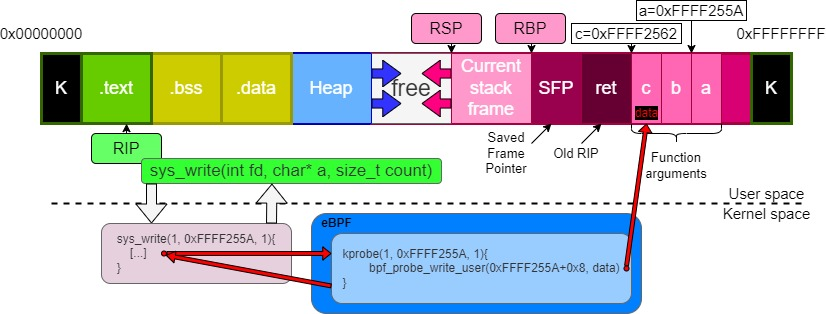
\includegraphics[width=16cm]{stack_scan_write_tech.jpg}
	\caption{Overview of stack scanning and writing technique.}
	\label{fig:stack_scan_write_tech}
\end{figure}

The above figure shows process memory executing a program similar to the following:
\begin{lstlisting}[language=C, caption={Sample program being executed on figure \ref{fig:stack_scan_write_tech}.}, label={code:stack_scan_write_tech}]
void func(char* a, char* b, char* c){
	int fd = open("FILE", 0);
	write(fd, a, 1);
}

int main(){
	char a[] = "AAA";
	char b[] = "BBB";
	char c[] = "CCC";
	func(a, b, c);
}
\end{lstlisting}

In the figure, we can clearly observe how the technique is used to overwrite an specific buffer. The attacker goal is to overwrite buffer \textit{c} with some other bytes, but the kprobe program only has direct access to buffer \textit{a}:
\begin{enumerate}
\item By reverse engineering the program (we will see how this process works in section \ref{TODO}) we notice that buffer \textit{c} is stored 8 bytes lower on the stack than buffer \textit{a}.
\item When register rip points to the write() instruction, the processor executes the instruction and a system call is issued to sys\_write().
\item The kprobe eBPF program hooked to the syscall hijacks the program execution. Since it has access to the memory address of buffer \textit{a} and it knows the relative position of buffer \textit{c}, it writes to that location whatever it wants (e.g.: "DDD") with the bpf\_probe\_write\_user() helper.
\item The eBPF program ends and the control flow goes back to the system call. It ends its execution successfully, and returns a value to the user space. The result of the program is that 1 byte has been written into file "FILE", and that buffer \textit{c} now contains "DDD".
\end{enumerate}

\subsection{Takeaways}
As a summary, the bpf\_probe\_write\_user() helper is one of the main attack vectors for malicious eBPF programs. Although it does contain some restrictions, its ability to overwrite any user parameter enables it to, in practice, execute arbitrary code by hijacking that of others. When it is combined with tracing programs' ability to read memory out of bounds, it unlocks a wide range of attacks, since any writeable section of the process memory is a possible target. 

Therefore, if on the conclusion of section \ref{subsection:tracing_attacks_conclusion} we discussed that the ability to change the return value of kernel functions and kill processes hinders the trust between the user and kernel space (since what the kernel returns may not be a correct result), then the ability to directly overwrite process data is a complete disrupt of trust in any of the data in the user space itself, since it is subject to the control of a malicious eBPF program.

Moreover, in the next sections we will discuss how we can create advanced attacks on the basis of the background and techniques previously discussed. We will research further into which sections of a process memory are writeable and whether they can lead to new attack vectors.


\section{Abusing networking programs}\label{section:abusing_networking}
The final main piece of a malicious eBPF program comes from taking advantage of the networking capabilities of TC and XDP programs. As we mentioned during sections \ref{subsection:xdp} and \ref{subsection:tc}, these type of programs have access to network traffic:
\begin{itemize}
\item Traffic Control programs can be placed either on egress or ingress traffic, and receive a struct \textit{sk\_buff}, containing the packet bytes and meta data that helps operating on it.
\item External Data Path programs can only be attached to ingress traffic, but in turn they receive the packet before any kernel processing (as a struct \textit{xdp\_md}) being able to access the raw data directly.
\end{itemize}

Networking eBPF programs not only have read access to the network packets, but also write access:
\begin{itemize}
\item XDP programs can directly modify the raw packet via memcpy() operations. They can also increment or reduce the size of the packet at any of its ends (adding bytes before the head or after the packet tail). This is done via the multiple helpers previously presented on table \ref{table:xdp_helpers}.
\item TC programs can also modify the packet via the helpers presented on table \ref{table:tc_helpers}. The packet can be expanded or reduced via these eBPF helpers too.
\end{itemize} 

Apart from write access to the packet, the other critical feature of networking programs is their ability to drop packets. As we presented in tables \ref{table:xdp_actions_av} and \ref{table:tc_actions}, this can be achieved by returning specific values.


\subsection{Attacks and limitations of networking programs}
Based on the previous background, we will now proceed to explore which limitations exist on which actions a network eBPF program can perform:
\begin{itemize}
\item Read and write access to the packet is heavily controlled by the eBPF verifier. It is not possible to read or write data out of bounds. Extreme care must also be taken before attempting to read any data inside the packet, since the verifier first requires making lots of checks beforehand. For any access to take place, the program must first classify the packet according to the network protocol it belongs, and later check that every header of every layer is well defined (e.g: Ethernet, IP and TCP). Only after that, the headers can be modified. 

If the program also wants to modify the packet payload, then it must be checked to be between the bounds of the packet and well defined according to the packet headers(using fields IHL, packet length and data offset, in figure \ref{fig:frame}). Also, after using any of the helpers that enlarge or reduce the size of the packet, all check operations must be repeated again before any subsequent operation.

Finally, note that after any modification in the packet, some network protocols (such as IP and TCP) require to recalculate their checksum fields. 

\item XDP and TC programs are not able to create packets, they can only operate over existing traffic.

\item If an XDP program modifies an incoming packet, the kernel will not know about the original data, but if an egress TC program modifies a packet being sent, the kernel will be able to notice the modification.
\end{itemize}

Having the previous restrictions in mind, we can find multiple possible malicious uses of an XDP/TC program:
\begin{itemize}
\item \textbf{Spy all network connections} in the system. An XDP or TC ingress program can read any packet from any interface, therefore achieving a comprehensive view on which are the running communications and opened ports (even if protocols with encryption are being used) and gathering transmitted data (if the connection is also in plaintext).
\item \textbf{Hide arbitrary traffic} from the host. If an XDP program drops a packet, the kernel will not be able to know any packet was received in the first place. This can be used to hide malicious incoming traffic. However, as we will mention in section{TODO}, malicious traffic may still be detected by other external devices, such as network-wide firewalls.
\item \textbf{Modify incoming traffic} with XDP programs. Every packet can be modified (as we mentioned at the beginning of section \ref{section:abusing_networking}), and any modification will be unnoticeable to the kernel, meaning that we will have complete, invisible control over the packets received by the kernel.
\item \textbf{Modify outgoing traffic} with TC egress programs. Since every packet can be modified at will, we will therefore have complete control over any packet sent by the host. This can be used to enable a malicious program to communicate over the network and exfiltrate data, since even if we cannot create a new connection from eBPF, we can still modify existing packets, writing any payload and headers on it (thus being able to, for instance, change the destination of the packet).

Notice, however, that these modifications are not transparent to the kernel as with XDP, and thus an internal firewall may detect our malicious traffic.
\end{itemize}

Although we mention the possibility of modifying outgoing traffic as an alternative to the impossibility of sending new packets from eBPF, there exists a major disadvantage by doing this, since the original packet of the application will be lost, and we will thus be disrupting the normal functioning of the system (which in a rootkit is unacceptable, as we mentioned in section \ref{section:motivation}, stealth is a priority).

There exists, however, a simple way of duplicating a packet so that the original packet is not lost but we can still send our overwritten packet. This technique, first presented by Guillaume Fournier and Sylvain Afchainthe in their DEFCON talk, consists of taking advantage of TCP retransmissions we described on section \ref{subsection:tcp}. Figure \ref{fig:tcp_exfiltrate_retrans} shows this process:

\begin{figure}[H]
	\centering
	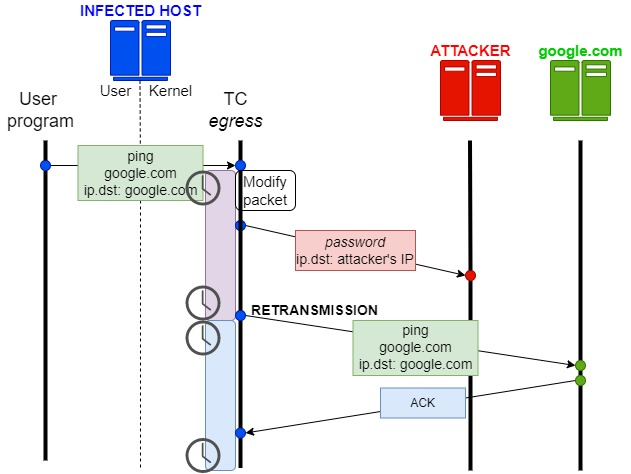
\includegraphics[width=15cm]{tcp_exfiltrate_retrans.jpg}
	\caption{Technique to duplicate a packet for exfiltrating data.}
	\label{fig:tcp_exfiltrate_retrans}
\end{figure}

In the figure, we can observe a host infected by a malicious TC egress program. An user space application at some point needs to send a packet (in this case a simple ping), and the TC program will overwrite it (in this case, it writes a password which it has been able to find, and substitutes the destination IP address with that of a listening attacker.
After the timer runs out, the TCP protocol itself will retransmit the same packet as previously and thus the original data is delivered too.

Using this technique, we will be able to send our own packets every time an application sends outgoing traffic. And, unless the network is being monitored, this attack will go unnoticed, provided that the delay of the original packet is similar to that when a single packet lost.

\subsection{Takeaways}
As a summary, networking eBPF programs offer complete control over incoming and outgoing traffic. If tracing programs and memory corruption techniques served to disrupt the trust in the execution of both any user or kernel program, then a malicious networking program has the potential to do the same with any communication, since any packet is under the control of eBPF.

Ultimately, the capabilities discussed in this section unlock complete freedom for the design of malicious programs. As we will explain in the next chapter, one particularly relevant type of application can be built:
\begin{itemize}
\item A \textbf{backdoor}, a stealthy program which listens on the network interface and waits for secret instructions from a remote attacker-controlled client program. This backdoor can have \textbf{Command and Control (C2)} capabilities, meaning that it can process commands sent by the attacker and received at the backdoor, executing a series of actions corresponding to the request received, and (when needed) answering the attacker with the result of the command.
\end{itemize}

%TODO maybe a conclusion for this section?

\chapter{Design of a malicious eBPF rootkit}
In the previous chapter, we discussed the functionality of eBPF programs from a security standpoint, detailing which helpers and program types are particularly useful for developing malicious programs, and analysing some techniques (stack scanning, overwriting packets together with TCP retransmissions) which helps us circumvent some of the restrictions of eBPF and find new attack vectors.

Taking as a basis these capabilities, this chapter is now dedicated to a comprehensive description of the advanced techniques and functionalities implemented in our eBPF rootkit, which show how these capabilities can lead to the creation of a real malicious application. As we mentioned during the project objectives, our goals for our rootkit include the following:
\begin{itemize}
\item Hijacking the execution of user programs while they are running, injecting libraries and executing malicious code, without impacting their normal execution.
\item Featuring a command-and-control module powered by a network backdoor, which can be operated from a remote client. This backdoor should be controlled with stealth in mind, featuring similar mechanisms to those present in rootkits found in the wild.
\item Tampering with user data at system calls, resulting in running malware-like programs and for other malicious purposes.
\item Achieving stealth, hiding rootkit-related files from the user.
\item Achieving rootkit persistence, the rootkit should run after a complete system reboot.

\end{itemize}
%TODO maybe this is the place to mention that, on top of those, explaining some of the DEFCON techniques will be done too. Im particular interested on the one of hiding the kernel log message of bpf_probe_write_user and on ROP.

We will be exploring each functionality individually, presenting the necessary background on each of them, and offering a final comprehensive view on how each of the systems work.

\section{Library injection attacks}
In this section, we will discuss how to hijack an user process running in the system so that it executes arbitrary code instructed from an eBPF program. For this, we will be injecting a library which will be executed by taking advantage of the fact that the GOT section in ELFs is flagged as writable (as we introduced in section \ref{subsection:elf_lazy_binding} and using the stack scanning technique covered in section \ref{subsection:bpf_probe_write_apps}. This injection will be stealthy (it must not crash the process), and will be able to hijack privileged programs such as systemd, so that the code is executed as root.

We will also research how to circumvent the protections which modern compilers have set in order to prevent similar attacks (when performed without eBPF).

This technique has some advantages and disadvantages to the one described by Jeff Dileo at DEFCON 27\cite{evil_ebpf_p6974}, which we will briefly cover before presenting ours. Both techniques will be later compared in section \ref{TODO EVALUATION}.


\subsection{ROP with eBPF} \label{subsection:rop_ebpf}
In 2019, Jeff Dileo presented in DEFCON 27 the first technique to achieve arbitrary code execution using eBPF\cite{evil_ebpf_p6974}. For this, he used the ROP technique we described in section \ref{subsection:rop} to inject malicious code into a process. We will present an overview on his technique, in order to later compare it to the one we will develop for our rootkit, and find advantages and disadvantages. Note that this is a summary and some aspects have been simplified, however we will go in full detail during the explanation of our own technique.

\begin{figure}[H]
	\centering
	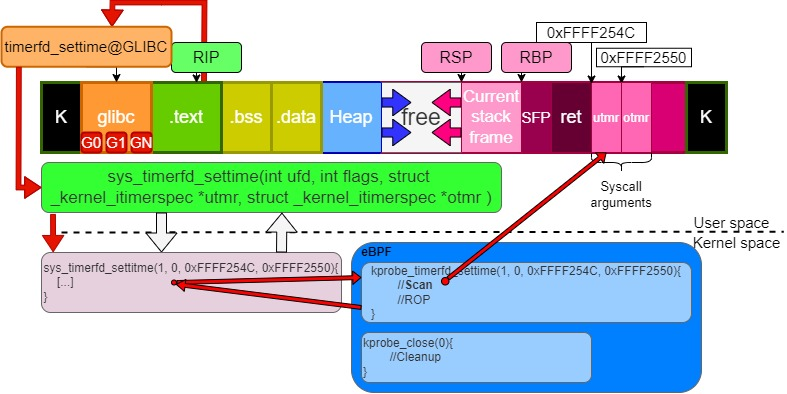
\includegraphics[width=15cm]{rop_evil_ebpf_1.jpg}
	\caption{Initial setup for the ROP with eBPF technique.}
	\label{fig:rop_evil_ebpf_1}
\end{figure}

Figure \ref{fig:rop_evil_ebpf_1} shows an overview on the process memory and the eBPF programs loaded. For this injection, we will use the stack scanning technique (section \ref{subsection:bpf_probe_write_apps}) using the arguments of a system call whose arguments are passed using the stack (sys\_timerfd\_settime, which receives two structs utmr and otmr). Therefore, a kprobe is attached to the system call, so that it can start to scan for the return address of the system call, which we know is the original value of register rip which was pushed into the stack (ret).

%TODO Maybe the glibc bit, because of its importance, is better somewhere else
An additional aspect must be introduced now (we will cover it more in detail in section \ref{TODO}): system calls are not directly called by the instructions in the .text section, but rather user programs in C make use of the C Standard Library to delegate the actual syscall, which in this case is the GNU Standard Library (glibc)\cite{glibc}. Therefore, a program calls a function in glibc (in this case timerfd\_settime) in which the syscall is performed, and the kernel executes it.

This means that, during the stack scanning technique, if we start from struct utmr and scan forward in the stack, what we will find in ret is the return address of the function of glibc, and not directly that of the syscall to the kernel. Therefore, our goal is, for every data in the stack while scanning forward, check whether it is the real return address of glibc. For an address to be the real return address, we will follow the next steps:
\begin{enumerate}
\item Take an address from the stack. If that is the return address (the old rip), then the instruction that called the function in glibc must be the previous instruction (rip - 1).
\item We now have a \textit{call} instruction, that directs us to the function at glibc. We check in the instruction to which address it moves the flow of execution, that is the address of timerfd\_settime in glibc.
\item We scan forward, inside timerfd\_settime of glibc, until we find a \textit{syscall} instruction. That is the point where the flow of execution moves to the kernel, so we have checked that the return address we found in the stack truly is the one we are looking for.
\end{enumerate}

Now that we have found the return address, we save a backup of the stack (to recover the original data later) and we proceed to overwrite the stack using bpf\_probe\_write\_user(), setting it for the ROP technique. For this, some gadgets (G0, G1 ... GN) have been previously discovered in the glibc library. Figure \ref{fig:rop_evil_ebpf_2} shows process memory after this overwrite:

\begin{figure}[H]
	\centering
	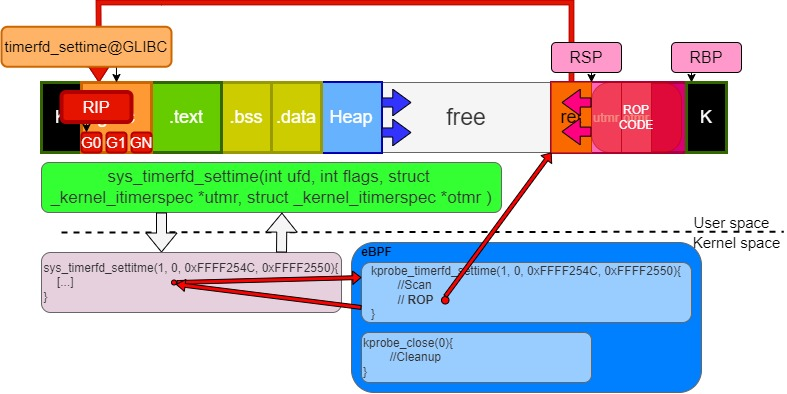
\includegraphics[width=15cm]{rop_evil_ebpf_2.jpg}
	\caption{Process memory after syscall exits and ROP code overwrites the stack.}
	\label{fig:rop_evil_ebpf_2}
\end{figure}

As we can see in the figure, the function has already exited, and ret has been popped into register rip. As we explained in section \ref{subsection:rop}, the attacker places in that position the address of the first ROP gadget. After that, the attacker can execute arbitrary code. Jeff Dileo, for instance, loads a malicious library into the process (we will do the same and explain this process in the next sections).

Once the attacker has finished executing the injected code, the stack must be restored to the original position so that the program can continue without crashing. A simplified view of this procedure consists of attaching a kprobe to a random system call (in this case, sys\_close()) so that, from the ROP code, we can alert the eBPF program when it is time to remove the ROP code and restore the original stack. Figure \ref{fig:rop_evil_ebpf_3} shows this final step:

\begin{figure}[H]
	\centering
	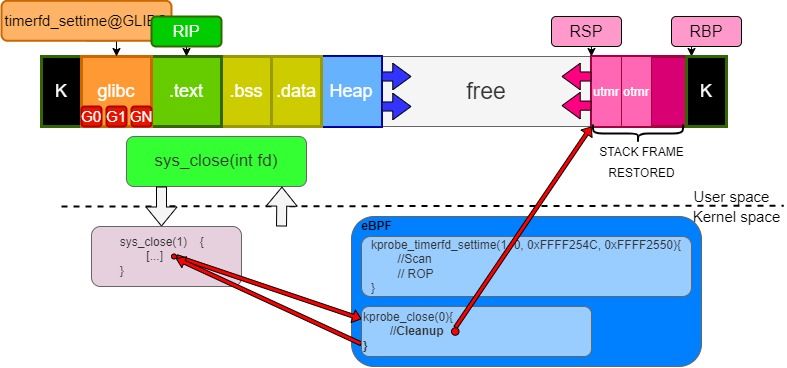
\includegraphics[width=15cm]{rop_evil_ebpf_3.jpg}
	\caption{Stack data is restored and program continues its execution.}
	\label{fig:rop_evil_ebpf_3}
\end{figure}

As we can see, eBPF writes back the original stack and thus the execution can continue. Note that, in practice, some final gadgets must also be executed in order to restore the state of rip and rsp, the stack data for this is written in the free memory zone, so that it does not need to be removed.


%TODO Eligible to writing more. This was merged with the explanation of each feature before, so it was more extense, but now it might need some more info??
\subsection{Bypassing hardening features in ELFs}
During section \ref{subsection:hardening_elf}, we presented multiple  security hardening measures that have been introduced to prevent common exploitation techniques (such as stack buffer overflows) and that nowadays can be incorporated, usually by default, in ELF binaries generated using modern compilers. We will now explore how to bypass these features, so that we can later design an injection technique that can target any process in the system, independently on whether it was compiled using these mitigations.

\textbf{Stack canaries}\\
Since stack canaries will be checked after the vulnerable function returns, an attacker seeking to overwrite the stack must ensure that the value of the canary remains constant. In the context of a buffer overflow attack, this can be achieved by leaking the value of the canary and incorporating it into the overflowing data at the stack, so that the same value is written on the same address\cite{canary_exploit}.

In our rootkit, unlike in the ROP technique presented in section \ref{subsection:rop_ebpf}, we will avoid overwriting the value of the saved rip in the stack completely. Therefore, as long as our eBPF program leaves all registers and stack data in the same state as before calling the function, we will not trigger any alerts.

\textbf{DEP/NX}\\
The only alternative for an attacker upon a non-executable stack is either injecting shellcode at any other executable memory address, or the use of advanced techniques like ROP that fully circumvent this mitigation since the data at the stack is not directly executed at any step.

In our rootkit, we will choose the first option, scanning the process virtual memory for an executable page where we will inject our shellcode. This process is usually known as finding 'code caves'.

\textbf{ASLR}\\
In order to bypass ASLR, attackers must take into account that, although the address at which, for instance, a library is loaded is random, the internal structure of the library remains unchanged, with all symbols in the same relative position, as figure \ref{table:aslr_offset} shows.

%TODO Add the .data section here
\begin{figure}[H]
	\centering
	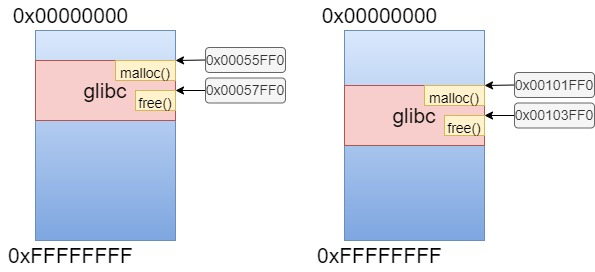
\includegraphics[width=13cm]{aslr_offset.jpg}
	\caption{Two runs of the same executable using ASLR, showing a library and two symbols.}
	\label{fig:alsr_offset}
\end{figure}

As we can observe in the figure, although glibc is loaded at a different base address each run, the offset between the functions it implements, malloc() and free(), remains constant. Therefore, a method for bypassing ASLR is to gather information about the absolute address of any symbol, which can then easily lead to knowing the address of any other if the attacker decompiles the executable and calculates the offset between a pair of addresses where one is known. This is the chosen method for our technique.

\textbf{PIE}\\
Similarly to ASLR, although the starting base address of each memory section is random, the internal structure of each section remains the same. Therefore, if an attacker is able to leak the address of some symbol in a section, and by knowing the offset at which it is located with respect to the base address of the section, then the address of any other symbol in the same section can be calculated\cite{pie_exploit}. This is the technique we will incorporate in our rootkit.

\textbf{RELRO}\\
If an executable was compiled using Partial RELRO, then the value of GOT can still be overwritten. If in turn it was compiled using Full RELRO, this stops any attempt of GOT hijacking, unless an attacker finds an alternative method for writing into the virtual memory of a process that bypasses the read-only flag. 

In our rootkit, we will directly write using eBPF the value of GOT if it was compiled with Partial RELRO, and use an alternative technique for writing into the virtual memory of a process whenever it was compiled using Full RELRO.


\subsection{Library injection via GOT hijacking} \label{subsection:got_attack}
Taking into account the background about stack attacks, ELF's lazy binding and hardening features for binaries we presented in section \ref{section:elf}, we will now present the exploitation technique incorporated in our rootkit to inject a malicious library into a running process. 

This attack is based on the possibility of overwriting the data at the GOT section. As we have mentioned previously, this section is marked as writeable if the program was compiled using Partial RELRO, meaning that we will be able to overwrite its value from an eBPF program using the helper bpf\_probe\_write\_user(). After modifying the value of GOT, a PLT stub will take the new value as the jump address (as we explained in section \ref{subsection:elf_lazy_binding}), effectively hijacking the flow of execution of the program. In the case that a program was compiled with Full RELRO (which will be the case of many programs running by default in a Linux system such as systemd), we will make use of the /proc filesystem for overwriting this value.

The rootkit will inject the library only after the second time that an specific syscall is called by a process, since the first time we will wait for the GOT address to be loaded by the dynamic linker. This is a necessary step because eBPF will need to validate that it really is the GOT section to overwrite.

This technique works both in compilers with low hardening fetaures by default (Clang) and also on a compiler with all of them active (GCC), see table \ref{table:compilers}. On each of the steps, we will detail the different existing methods depending on the compiler features.

For this research work, the rootkit is prepared to perform this attack on any process that makes use of either the system call sys\_openat or sys\_timerfd\_settime, which are called by the standard library glibc.

\textbf{Stage 1: eBPF tracing and scan the stack}\\
We load and attach a tracepoint eBPF program at the \textit{enter} position of syscall sys\_timerfd\_settime. Firstly we must ensure that the process calling the tracepoint is one of the processes to hijack.

We will then proceed with the stack scanning technique, as we explained in section \ref{subsection:bpf_probe_write_apps}. In this case, the algorithm will go as follows:
\begin{enumerate}
\item Take one of the syscall parameters and scan forward in the scan. For each iteration, we must check if the data at the stack corresponds to the saved rip:
\begin{enumerate}
\item Check that the previous instruction is a call instruction, by checking the instruction length and opcodes (call instructions always start with e8, and the length is 5 bytes, see figure \ref{fig:firstcall}).
\begin{figure}[H]
	\centering
	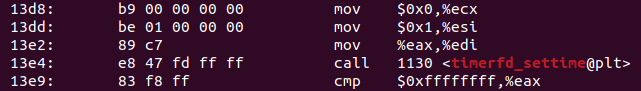
\includegraphics[width=13cm]{sch_firstcall.png}
	\caption{Call to the glibc function, using objdump}
	\label{fig:firstcall}
\end{figure}
\item Now that we know we localized a call instruction, we take the address at which it jumps. That should be an address in a PLT stub.
\item We analyze the instruction at the PLT stub. If the program was compiled with GCC, it will be an \textit{endbr64} instruction followed by the PLT jump instruction using the address at GOT (since it generates Intel CET-compatible programs, see table \ref{table:compilers}). Otherwise, if using Clang, the first instruction is the PLT jump.
%TODO Continue
\end{enumerate}
\end{enumerate}
\chapter{Evaluation} \label{chapter:evaluation}
This chapter evaluates the malicious capabilities developed in our rootkit by comparing them to the original objectives we presented at the beginning of our research in section \ref{section:project_objectives}. For this, we will analyse whether our rootkit meets the expected functionality by simulating a machine infection in a virtualized environment. A rootkit functionality will be considered fulfilled in the case it can be reproduced successfully in the experimental environment.

As we mentioned, the following are the functionalities we seeked to implement in our rootkit:
\begin{itemize}
\item Hijacking the execution of user programs while they are running, injecting libraries and executing malicious code, without impacting their normal execution.
\item Featuring a command-and-control module powered by a network backdoor, which can be operated from a remote client. This backdoor should be controlled with stealth in mind, featuring similar mechanisms to those present in rootkits found in the wild.
\item Tampering with user data at system calls, resulting in running malware-like programs and for other malicious purposes.
\item Achieving stealth, hiding rootkit-related files from the user.
\item Achieving rootkit persistence, the rootkit should run after a complete system reboot.
\end{itemize}

\section{Experimental setting}
The test environment that will be used to showcase the rootkit functionalities consists on two virtual machines running under Oracle VM VirtualBox \cite{virtualbox_page}. One of them will be the host infected with the rootkit, while the other will be used as the attacker machine from which to operate the rootkit client. 

Both virtual machines will be connected via a bridged adapter, as figure \ref{fig:vm_setting_bridged} shows. With this virtual networking setting, the virtual machines connect to a device driver of the host system which injects the data received from the physical network \cite{bridged_networking}. From the virtual machine point of view, both the attacker and the infected machine appear to be physically connected (via a network cable) to the same network interface, each with a different assigned IP address. The name of this interface will be "enp0s3".

\begin{figure}[htbp]
	\centering
	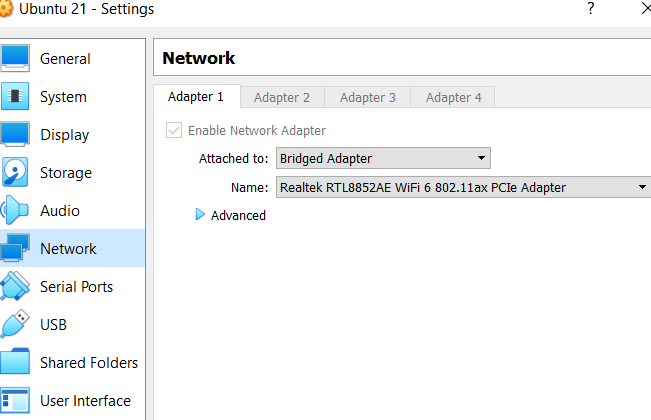
\includegraphics[width=13cm]{vm_setting_bridged.png}
	\caption{Network settings for both of the VMs on the test environment.}
	\label{fig:vm_setting_bridged}
\end{figure}

Table \ref{table:vm_config_test_environment} shows the role and charactersitics of the two machines. The overall test environment configuration with the described settings is illustrated in figure \ref{fig:test_env}.

\begin{table}[H]
\begin{tabular}{|>{\centering\arraybackslash}p{3cm}|>{\centering\arraybackslash}p{3cm}|}
\hline
\multicolumn{2}{|c|}{\textbf{INFECTED MACHINE}}\\
\hline
\textbf{Attribute} & \textbf{Value}\\
\hline
\hline
User & osboxes\\
\hline
Operating System & GNU/Linux\\
\hline
Distribution & Ubuntu 21.04\\
\hline
Kernel version & 5.11.0-49\\
\hline
IP address & 192.168.1.124\\
\hline
\end{tabular}
\quad
\begin{tabular}{|>{\centering\arraybackslash}p{3cm}|>{\centering\arraybackslash}p{3cm}|}
\hline
\multicolumn{2}{|c|}{\textbf{ATTACKER MACHINE}}\\
\hline
\textbf{Attribute} & \textbf{Value}\\
\hline
\hline
User & RED\\
\hline
Operating System & GNU/Linux\\
\hline
Distribution & Ubuntu 18.04\\
\hline
Kernel version & 5.4.0-96\\
\hline
IP address & 192.168.1.121\\
\hline
\end{tabular}
\caption{Configuration of virtual machines in the test environment.}
\label{table:vm_config_test_environment}
\end{table}

\begin{figure}[htbp]
	\centering
	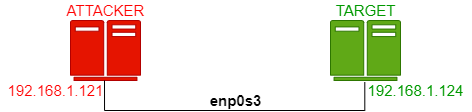
\includegraphics[width=13cm]{test_env.png}
	\caption{Network topology of test environment.}
	\label{fig:test_env}
\end{figure}


%Maybe this is not the place for story telling? I thought that telling it like this fits nicely here to put some context, but I can try to change it.
\section{Attack scenario} \label{section:attack_scenario}
This section presents an hypothetical attack scenario, covering each of the steps the attacker must follow in order to prepare the rootkit and infect a machine:

A security researcher called 'RED' has managed to exploit a high-severity RCE vulnerability in a critical system controlled by an adversary which was found exposed to the Internet (e.g.: not behind a NAT \cite{nat_comptia}). After this exploitation, RED has now spawned a reverse shell connection with the privileged user 'osboxes', but he knows that the system is often rebooted and that he may lose access soon. Furthermore, the vulnerability he exploited is already well-known and may get patched in the near future, so he needs to persist his access. RED decides to load a classic rootkit consisting of a malicious kernel module, but he finds out that this capability is restricted in the system (e.g.: kernel.modules\_disabled=1 \cite{kernel_modules_restrict}), so he must find an alternative approach. At some point, RED realises that even if kernel modules were restricted, the system administrator did not block eBPF, so he decides to use TripleCross.

Firstly, RED creates a secret directory where to hide the rootkit, and downloads it, as shown in figure \ref{fig:post_exp}.

\begin{figure}[htbp]
	\centering
	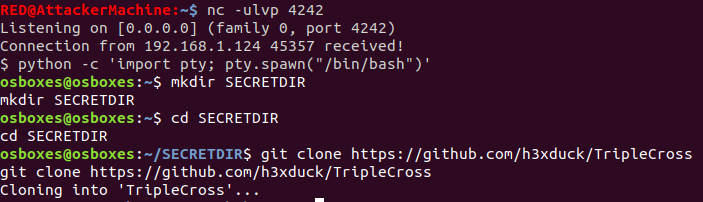
\includegraphics[width=13cm]{sch_post_exp.png}
	\caption{Creation of hidden directory and downloading rootkit.}
	\label{fig:post_exp}
\end{figure}

The rootkit C2 capabilities work out of the box, but RED wants to use all of the rootkit modules, so he must first make some configurations. Table \ref{table:rootkit_config} shows the configurations and the files to modify for each module.

\begin{table}[htbp]
\begin{tabular}{|>{\centering\arraybackslash}p{2cm}|>{\centering\arraybackslash}p{3cm}|>{\centering\arraybackslash}p{4cm}|>{\centering\arraybackslash}p{4cm}|}
\hline
\textbf{MODULE} & \textbf{FILENAME} & \textbf{CONSTANT} & \textbf{DESCRIPTION}\\
\hline
\hline
Execution hijacking & src/common/ constants.h & PATH\_EXECUTION\_HIJACK\_PROGRAM & Absolute path of malicious program\\
\hline
Privilege escalation & src/common/ constants.h & STRING\_FS\_SUDOERS\_ENTRY & Entry to inject in sudoers file\\
\hline
Library injection & src/helpers/ injection\_lib.h & ATTACKER\_IP \& ATTACKER\_PORT & IP address and port of attacker machine\\
\hline
Persistence module & src/helpers/ deployer.sh & CRON\_PERSIST \& SUDO\_PERSIST & Values to store at persistence files\\
\hline
\end{tabular}
\caption{Overall rootkit modules configuration.}
\label{table:rootkit_config}
\end{table}

Once the appropiate values have been written, RED executes the \textit{packager.sh} script, that will compile the rootkit. Alternatively, an attacker could have compiled it locally and sent it to the remote machine afterwards.

After the script execution finishes, a folder \textit{apps} is generated with all the rootkit files. This directory contains all the files and scripts needed for the rootkit installation. RED now executes the \textit{deployer.sh} script, which installs the rootkit and writes the persistence files, as shown in figure \ref{fig:deploy_root}

\begin{figure}[htbp]
	\centering
	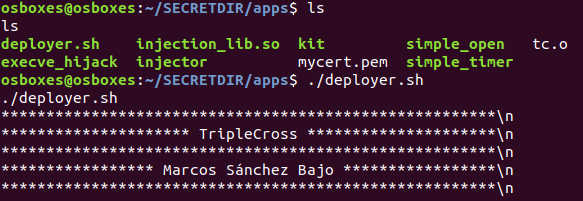
\includegraphics[width=13cm]{sch_deploy_root.png}
	\caption{Files created by packager.sh and execution of deployer.sh.}
	\label{fig:deploy_root}
\end{figure}

Once the script has been executed, all rootkit modules are loaded and the backdoor is already waiting for commands. RED can now close the reverse shell and open the rootkit client. He now has persistent privileged access to the infected machine.

\section{Hijacking execution of running processes}
Following the infection process described in section \ref{section:attack_scenario}, TripleCross can hijack the execution of running processes by means of the library injection module. This module incorporates two sample programs (\textit{src/helpers/simple\_timer.c and src/helpers/simple\_open.c}), both containing the execution of one of the hijacked syscalls (sys\_timerfd\_settime and sys\_openat respectively). Additionally, the functionality can be tested in any process of the infected machine by changing its settings. Table \ref{table:lib_injection_config} shows how to customize the functionality of the library injection module.

\begin{table}[htbp]
\begin{tabular}{|>{\centering\arraybackslash}p{3cm}|>{\centering\arraybackslash}p{5.5cm}|>{\centering\arraybackslash}p{5.5cm}|}
\hline
\textbf{FILENAME} & \textbf{CONSTANT} & \textbf{DESCRIPTION}\\
\hline
\hline
src/common/ constants.h & TASK\_COMM\_NAME\_INJECTION\_TARGET\_TIMERFD\_SETTIME & Name of process to hijack at syscall sys\_timerfd\_settime.\\
\hline
src/common/ constants.h & TASK\_COMM\_NAME\_INJECTION\_TARGET\_OPEN & Name of process to hijack at syscall sys\_openat.\\
\hline
src/helpers/ injection\_lib.c & ATTACKER\_IP \& ATTACKER\_PORT & IP address and port of attacker machine\\
\hline
\end{tabular}
\caption{Library injection module configuration.}
\label{table:lib_injection_config}
\end{table}

After a successful injection the malicious library will run a reverse shell against the attacker machine. Also, it will print a message for us to check it locally. Therefore, from the attacker machine, we will listen to the specified IP and port, considering the injection successful if a connection is opened.


\subsection{Test program simple\_timer}
Table \ref{table:lib_injection_config_simple_timer} shows the module configuration for running this attack.

\begin{table}[htbp]
\begin{tabular}{|>{\centering\arraybackslash}p{3cm}|>{\centering\arraybackslash}p{5.5cm}|>{\centering\arraybackslash}p{5.5cm}|}
\hline
\textbf{FILENAME} & \textbf{CONSTANT} & \textbf{VALUE}\\
\hline
\hline
src/common/ constants.h & TASK\_COMM\_NAME\_INJECTION\_TARGET\_TIMERFD\_SETTIME & "simple\_timer"\\
\hline
src/helpers/ injection\_lib.c & ATTACKER\_IP \& ATTACKER\_PORT & 192.168.1.127 \& 5555 \\
\hline
\end{tabular}
\caption{Library injection module configuration for attacking simple\_timer.c.}
\label{table:lib_injection_config_simple_timer}
\end{table}

Figure \ref{fig:sc_lib_inj_simple_timer_off} shows the execution of the simple\_timer process without the rootkit installed.

\begin{figure}[htbp]
	\centering
	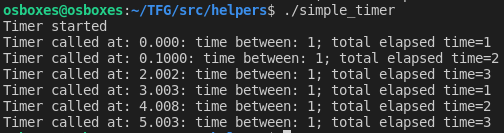
\includegraphics[width=13cm]{sch_sc_lib_inj_simple_timer_off.png}
	\caption{Normal execution of simple\_timer program.}
	\label{fig:sc_lib_inj_simple_timer_off}
\end{figure}

Once the rootkit is installed it starts the module automatically, looking for system calls from the simple\_timer process.
The attacker must in the mean time start a listener (e.g.: with netcat), as shown in figure \ref{fig:sc_lib_inj_nc}.

\begin{figure}[htbp]
	\centering
	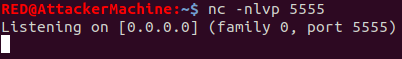
\includegraphics[width=12cm]{sch_sc_lib_inj_nc.png}
	\caption{Attacker waiting for a connection with netcat.}
	\label{fig:sc_lib_inj_nc}
\end{figure}

Then, the simple\_timer program gets executed on the infected machine. As we can observe in figure \ref{fig:sc_lib_inj_simple_timer_exec}, the injection suceeds and a message is printed from the library. 

\begin{figure}[htbp]
	\centering
	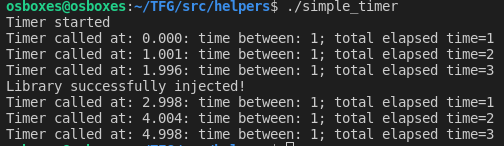
\includegraphics[width=12cm]{sch_sc_lib_inj_simple_timer_exec.png}
	\caption{Execution of simple\_timer.c with rootkit active.}
	\label{fig:sc_lib_inj_simple_timer_exec}
\end{figure}


Figure \ref{fig:sc_lib_inj_nc_success} shows the attacker connected to the reverse shell launched from the library.

\begin{figure}[htbp]
	\centering
	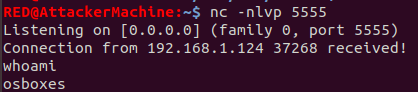
\includegraphics[width=12cm]{sch_sc_lib_inj_nc_success.png}
	\caption{Reverse shell received after library injection attack.}
	\label{fig:sc_lib_inj_nc_success}
\end{figure}


\subsection{Test program simple\_open}
The library injection module can also be tested with the simple\_timer program, which opens multiple files with sys\_openat. The rootkit configuration for this is shown in table \ref{table:lib_injection_config_simple_open}.

\begin{table}[htbp]
\begin{tabular}{|>{\centering\arraybackslash}p{3cm}|>{\centering\arraybackslash}p{5.5cm}|>{\centering\arraybackslash}p{5.5cm}|}
\hline
\textbf{FILENAME} & \textbf{CONSTANT} & \textbf{VALUE}\\
\hline
\hline
src/common/ constants.h & TASK\_COMM\_NAME\_INJECTION\_TARGET\_OPEN & "simple\_open"\\
\hline
src/helpers/ injection\_lib.c & ATTACKER\_IP \& ATTACKER\_PORT & 192.168.1.127 \& 5555 \\
\hline
\end{tabular}
\caption{Library injection module configuration for attacking simple\_open.c.}
\label{table:lib_injection_config_simple_open}
\end{table}

As we can observe in figure \ref{fig:sc_lib_inj_simple_open}, when the injection suceeds, a message is printed on screen. Also, the attacker receives a shell, like we showed in figure \ref{fig:sc_lib_inj_nc_success}.

\begin{figure}[htbp]
	\centering
	
\includegraphics[width=12cm]{sch_sc_lib_inj_simple_open.png}
	\caption{Execution of simple\_open with rootkit active.}
	\label{fig:sc_lib_inj_simple_open}
\end{figure}


\subsection{Hijacking systemd}
Apart from the test programs, the library injection module can also inject the malicious library on any process of the system that makes use of either sys\_openat or sys\_timerfd\_settime. By hijacking privileged system programs such as systemd, the malicious library can achieve automatic root permissions once it is run (although these are anyways automatically granted via the privilege escalation module). Table \ref{table:lib_injection_config_systemd} shows the module configuration for running an attack against this process.

\begin{table}[htbp]
\begin{tabular}{|>{\centering\arraybackslash}p{3cm}|>{\centering\arraybackslash}p{5.5cm}|>{\centering\arraybackslash}p{5.5cm}|}
\hline
\textbf{FILENAME} & \textbf{CONSTANT} & \textbf{VALUE}\\
\hline
\hline
src/common/ constants.h & TASK\_COMM\_NAME\_INJECTION\_TARGET\_TIMERFD\_SETTIME & "systemd"\\
\hline
src/common/ constants.h & TASK\_COMM\_NAME\_INJECTION\_TARGET\_OPEN & "systemd"\\
\hline
src/helpers/ injection\_lib.c & ATTACKER\_IP \& ATTACKER\_PORT & 192.168.1.127 \& 5555 \\
\hline
\end{tabular}
\caption{Library injection module configuration for attacking the systemd process.}
\label{table:lib_injection_config_systemd}
\end{table}

With these configurations, we can run the rootkit and wait for systemd to call one of these syscalls. Eventually this call occurs, and using the debug messages of the rootkit we can get information on what happened, as shown in figure \ref{fig:sch_sc_lib_inj_systemd_debug}.

\begin{figure}[htbp]
	\centering
	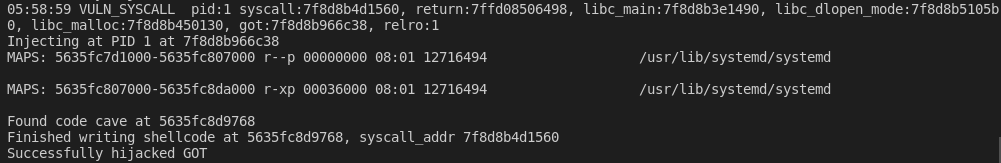
\includegraphics[width=12cm]{sch_sc_lib_inj_systemd_debug.png}
	\caption{Rootkit debug messages showing library injection.}
	\label{fig:sc_lib_inj_systemd_debug}
\end{figure}

As we can observe in the figure, the rootkit finds the relevant addresses via the technique we described on section \ref{section:lib_injection} and proceeds to overwrite the GOT address. The library is loaded and executed, and since systemd is executed by the root user, the attacker receives a root shell as shown in figure \ref{fig:lib_inj_success_root}. Most importantly, the systemd process does not crash after this attack.

\begin{figure}[htbp]
	\centering
	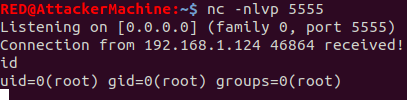
\includegraphics[width=12cm]{sch_lib_inj_success_root.png}
	\caption{Reverse shell received with root user after systemd library injection.}
	\label{fig:lib_inj_success_root}
\end{figure}


\section{Backdoor and C2}
The backdoor module works out of the box without any additional configurations needed. It includes the C2 capabilities and the rootkit client used to communicate with the backdoor. As we described in section \ref{subsection:rootkit_manual}, the client allows for the operations listed on table \ref{table:rootkit_client_actions}.

\begin{table}[htbp]
\begin{tabular}{|>{\centering\arraybackslash}p{5cm}|>{\centering\arraybackslash}p{9.5cm}|}
\hline
\textbf{PROGRAM ARGUMENTS} & \textbf{ACTION DESCRIPTION}\\
\hline
\hline
./injector -c <Victim IP> & Spawns a plaintext pseudo-shell by using the execution hijacking module.\\
\hline
./injector -e <Victim IP> & Spawns an encrypted pseudo-shell by commanding the backdoor with a pattern-based trigger.\\
\hline
./injector -s <Victim IP> & Spawns an encrypted pseudo-shell by commanding the backdoor with a multi-packet trigger (of both types).\\
\hline
./injector -p <Victim IP> & Spawns a phantom shell by commanding the backdoor with a pattern-based trigger.\\
\hline
./injector -a <Victim IP> & Orders the rootkit to activate all eBPF programs.\\
\hline
./injector -a <Victim IP> & Orders the rootkit to detach all of its eBPF programs.\\
\hline
./injector -S <Victim IP> & Showcases how the backdoor can hide a message from the kernel.\\
\hline
./injector -h & Displays help.\\
\hline
\end{tabular}
\caption{Rootkit client options.}
\label{table:rootkit_client_actions}
\end{table}

Once the rootkit is installed, the backdoor is launched automatically and will wait for backdoor triggers ready to launch the corresponding requested actions.

\subsection{Spawning encrypted pseudo-shells}
Encrypted pseudo-shells can be spawned using the rootkit client either with pattern-based or multi-packet backdoor triggers.

\textbf{Pattern-based triggers}\\
When using a pattern-based trigger, the attacker must indicate the following information:
\begin{itemize}
\item The IP address of the infected machine.
\item The network interface to use for sending the trigger.
\end{itemize}

As figure \ref{fig:sc_eps_rc} shows, the backdoor executes the requested action and starts an encrypted pseudo-shell connection with privileged permissions in which the attacker can introduce commands to be executed. Whenever the connection shall be closed, the attacker introduces the "EXIT" global command (as we explained in section \ref{subsection:rootkit_manual}), which ends the transmission gracefully.

\begin{figure}[htbp]
	\centering
	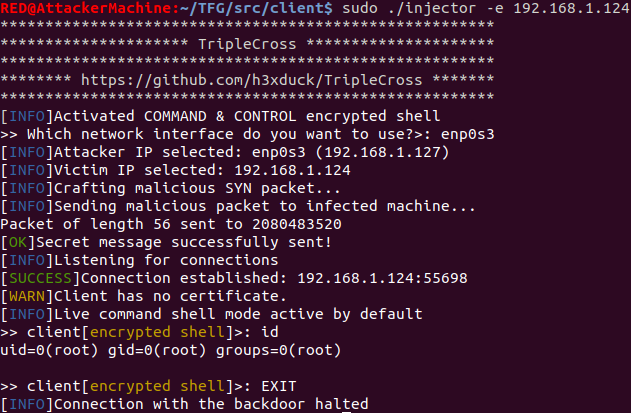
\includegraphics[width=12cm]{sch_sc_eps_rc.png}
	\caption{Encrypted pseudo-shell with rootkit client using pattern-based trigger.}
	\label{fig:sc_eps_rc}
\end{figure}

\textbf{Multi-packet triggers}\\
The rootkit client offers multiple options when using the multi-packet backdoor triggers. In particular, the attacker must specify the following fields:
\begin{itemize}
\item The IP address of the infected machine.
\item The network interface to use for sending the trigger.
\item Whether to hide the payload at the TCP sequence numbers or at the TCP source port.
\end{itemize}

Figure \ref{fig:sc_eps_seqnum} shows how the rootkit client asks for this data and spawns an encrypted pseudo-shell with the client when hiding the payload at the TCP sequence number. As we can observe in the figure, the payload is divided in 3 different chunks and injected to a stream of packets, which are sent in an orderly manner.

\begin{figure}[htbp]
	\centering
	\includegraphics[width=12cm]{sch_sc_eps_seqnum.png}
	\caption{Encrypted pseudo-shell with rootkit client using multi-packet trigger with payload hidden in TCP sequence number.}
	\label{fig:sc_eps_seqnum}
\end{figure}

Figure \ref{fig:sc_eps_srcport} shows the same process but using the TCP source port as a means for hiding the data payload. As we can observe in the figure, in this case the paylaod is divided in 6 chunks.

\begin{figure}[htbp]
	\centering
	\includegraphics[width=12cm]{sch_sc_eps_srcport.png}
	\caption{Encrypted pseudo-shell with rootkit client using multi-packet trigger with payload hidden in TCP source port.}
	\label{fig:sc_eps_srcport}
\end{figure}

\subsection{Spawning phantom shells}





\chapter{Related work} \label{chapter:related_work}
% Comparison of the rootkit with other eBPF and non eBPF rootkits.
In this work, we have developed a rootkit that loads itself in the kernel
and incorporates network-level capabilities and other functionalities both
at user and kernel space. Although eBPF, the technology used for this
rootkit, has been rarely explored before, some of the techniques presented
here are equivalent (or mimic) those historically incorporated in classic
rootkits, while others are also inspired by malicious uses of eBPF explored
in recent research. 

In this chapter, we provide a comprehensive review of previous
work on UNIX/Linux rootkits, their main types and most relevant examples.
We also offer a comparison in terms of techniques and functionality with
previous families. In particular, we highlight the differences of our
eBPF rootkit with respect to others that rely on traditional methods,
and also to those already built using eBPF.

\section{User-mode rootkits}
As discussed in Section \ref{section:motivation}, user-mode rootkits
are those that are run at the same level as common user applications. They
do not require to be loaded in the kernel to tamper with the execution of
programs. Instead, they usually redirect or substitute common system
programs to achieve their malicious purposes.

The most popular and commonly found technique in user-mode rootkits is the
LD\_PRELOAD technique, which enables to redefine function calls at shared
libraries. LD\_PRELOAD is an environment variable interpreted by the
dynamic linker at runtime that indicates to preload a shared library
before those already indicated at the ELF file \cite{ldpreload_pros}. If
this preloaded library implements the same function as some other library,
then the preloaded function overrides the original. This means that a
rootkit may define functions with malicious functionality that will run in
any program that loads the library instead of that from the original
function, without the need of modifying any of these programs.

This type of rootkits are considered trivial to detect by an investigator,
however they are easy to write and their capabilities can be quickly
extended, which has motivated the creation of many LD\_PRELOAD rootkits.

\subsection{Jynx/Jynx2} Jynx \cite{jynx_github} is one of the most
well-known rootkits using the LD\_PRELOAD technique. It injects the name of
its malicious library into the file \textit{/etc/ld.so.preload}, which acts
similarly to defining the LD\_PRELOAD environment variable for each
executable, but instead applying this setting to any program (since every
program checks this file to know the libraries to preload)
\cite{ldpreload_so_jynx}.

Its first version, Jynx, was best known for implementing a backdoor by
hooking the socket function accept() \cite{ldpreload_pros_2327}. This
function, responsible of accepting a connection, was defined in a preloaded
malicious library so that any connection (specifically encrypted ones)
could be checked to come from a remote attacker. If that is the case, the
rootkit would accept and establish a connection, and then execute a remote
root shell which provided the attacker with remote access.

In its later version, Jynx2 \cite{jynx2_github}, the rootkit incorporated
other mechanisms focused on hiding the rootkit activity
\cite{jynx2_infosecinstitute}. This included hiding Jynx's connections by
hooking read calls at the \textit{/proc} filesystem (which we covered in
Section \ref{section:proc_filesystem} so that processes related with the
rootkit activity remain undisclosed. Other functionalities include file
hiding, privilege escalation, or multi-factor authentication in the rootkit
backdoor.

\subsection{Azazel}
Azazel is another LD\_PRELOAD rootkit originally based on Jynx and that
extends its functionalities in multiple areas, including additional
anti-debugging and anti-detection techniques. This rootkit incorporates
more hooked functions into its preloaded library to achieve capabilities
such as:
\begin{itemize}
\item Avoid detection by programs such as \textit{ldd} (which lists
libraries to be loaded in an executable), \textit{ps} (which lists
processes) or \textit{lsof} (that displays opened files by processes).
\item Hide rootkit files and processes.
\item Hide rootkit-related network connections.
\item Incorporate backdoors (one launching an encrypted connection, another in plaintext).
\item Clean logs and allow for local privilege escalation.
\item Anti-debugging, by means of hooking ptrace() calls.
\end{itemize}

\subsection{TripleCross comparison}
Jynx---and, especially, Azazel---are advanced rootkits with many
functionalities, but they are restricted both because of the LD\_PRELOAD
technique and because of working from the user space.
%
In particular, the use of LD\_PRELOAD in a program can be detected by the
\textit{export} command and removed via \textit{unset}
\cite{ld_preload_detect}. In addition, this technique does not work on
statically-linked programs, that is, those where the calls to libraries
and exported functions are resolved at compile time \cite{ldpreload_pros}.
On the other hand, because they only have access to user-space programs and
components, their activities can be more easily detected than a rootkit
working from inside the kernel.

Since TripleCross is composed of both a kernel-side component (the eBPF
programs at the kernel) and a user-side component (the rootkit user program
that communicates with eBPF), the capabilities of user-mode rootkits are
more limited than those that could be eventually implemented in
TripleCross, yet they are easier and faster to implement, and do not
require loading an eBPF program in the kernel, an event which is likely to
be logged by EDRs and IDSs.

With respect to the capabilities offered, the ability to hook function
calls by preloading libraries so that malicious code is run can be
considered analogous to eBPF tracepoint, kprobe, and uprobes programs. On
the one hand, eBPF can modify parameters and execute kernel code
transparently from user programs. On the other hand, user-mode
rootkits may execute any instruction on the preloaded libraries, but eBPF
is restricted to a certain range of operations and those offered by eBPF
helpers. Nevertheless, both types of rootkits are able to implement the key
features needed for a usual rootkit, including a backdoor and a C2 system,
in addition to the basic stealth mechanisms.

\section{Kernel-mode rootkits}
As described in Section \ref{section:motivation}, kernel-mode
rootkits are run at the same level of privilege as the operating system,
thus enjoying unrestricted access in both the kernel- and user-space. These
are the hardest and riskiest to develop (since they need to work with
kernel structures and any error could cause a kernel panic), yet the offer
the richest and most powerful variety of functionalities. Also, they mostly
remain hidden from the user space, thus boosting their stealth, while at
the same time they are capable of further hiding their activities thanks
to their capabilities at both the user- and kernel-space.

Historically, kernel-mode rootkits in UNIX systems have been built as
Loadable Kernel Modules (LKM), whose original purpose is to expand the
capabilities of the kernel by adding new modules for specific tasks without
the need of recompiling or even reloading the kernel. 

\subsection{SucKIT rootkit}
Although the great majority of kernel-mode rootkits are loaded as LKMs,
SucKIT \cite{suckit_rootkit} remains one of the exceptions to this rule.
This old rootkit uses the \textit{/dev/kmem} special file \cite{dev_kmem}
for directly accessing kernel memory, including both reading and writing.
This means that the rootkit could potentially find and overwrite key data
at the kernel \cite{suckit_lasamhna}.

Nowadays, this type of rootkit is not relevant except for historical
reasons, since distributions such as Debian have limited access to this file to
kernels compiled with the CONFIG\_DEVKMEM parameter \cite{dev_kmem_debian}
which is disabled by default \cite{dev_kmem_off_default}.

\subsection{Diamorphine}
Diamorphine \cite{diamorphine_github} is one of the best known kernel-mode
rootkits, and it is implemented as a LKM. This type of rootkits commonly
intercept and hook system calls from the kernel, executing malicious code
(together with the original function) with the aim of achieving different
malicious purposes.

When a system call takes place in the user space, an interrupt is issued to
the kernel, which checks the type of syscall that has been issued. This is
done using a syscall table, which relates each system call to the function
at the kernel where its implementation is stored. A common technique by
LKMs is to modify the syscall table, so that it points to the functions
implemented by the LKM, where the malicious code will be executed
\cite{incibe_rootkit_lkm}. This code may be a modified version of the
original (e.g.: a sys\_getdents64 call that lists files but hides those
belonging to the rootkit) or modify kernel and user data received at the
hooked function.

Because LKMs are run directly inside the kernel, they are not limitied and thus
they can read, write and allocate kernel and user memory freely. It is also
possible to hook and modify data at internal kernel functions by means of,
for instance, kprobe programs.

In the case of Diamorphine, it uses the aforementioned capabilities to hide
processes, provide local privilege escalation, hide files and directories
and implement a messaging protocol using system calls (it enables a
malicious user to locally communicate actions to the rootkit with
\textit{kill} signals). Most importantly, it hides itself from commands
such as \textit{lsmod}, which list the LKMs loaded into the kernel, thus
turning invisible.

\subsection{Reptile}
Reptile \cite{reptile_github} is another LKM rootkit which incorporates
advanced stealth and network functionalities. Some of its most relevant
capabilities include:
\begin{itemize}
\item Hiding files, directories, processes and network connections related to the rootkit activity.
\item A backdoor that is operated via port-knocking triggers (which we explained in Section \ref{subsection:triggers}).
\item C2 capabilities via a custom shell (similar to the pseudo-shells of our rootkit).
\end{itemize}

\subsection{TripleCross comparison}
Although TripleCross incorporates many of the techniques mentioned in
Reptile and Diamorphine (backdooring, modification of files and directories
or local privilege escalation) these capabilities are achieved using
workarounds for the limitations of eBPF programs, namely not having write
access in kernel memory. For instance, Reptile can grant root privileges to
any program by overwriting the kernel data structure storing the user
privileges, whilst this is not achievable for TripleCross, which has to
take advantage of user buffers when reading the \textit{/etc/sudoers}
file.

Therefore, LKMs are more powerful since they enjoy almost no restrictions
in the kernel, while TripleCross' modules will always be limited to those
capabilities achievable without kernel memory modifications. In terms of
developing complexity, LKMs are more difficult to develop, since eBPF
programs will never crash the kernel (because of the eBPF verifier), whilst
developing kernel modules may incur in causing kernel panics, often because
of tiny kernel differences between kernel versions, which leads to having
to adjust the LKM for multiple kernels. On the other hand, although an eBPF
program is guaranteed to work once in the kernel, it requires deep
knowledge of which actions are accepted by the verifier, and about which
are the limitations of these programs.

With respect to the techniques used we can also find similarities, since
both LKMs and eBPF rootkits make heavy use of hooking syscalls and kernel
functions, with the only difference that the instructions that can be
executed at the eBPF probe function are restricted to those allowed by
the eBPF helpers, whilst LKMs may read or write any memory section. In
terms of network-related functions, both eBPF and LKMs enjoy similar
capabilities, with the exception that LKMs may create their own packets,
whilst eBPF may only modify or drop existing ones. Finally, both LKMs and
eBPF rootkits may execute user space programs (in eBPF, by hijacking calls
or triggering actions via a messaging system such as a ring buffer, and in
LKMs using, for instance, the function call\_usermodehelper
\cite{usermode_helper_lkm}).


\section{eBPF rootkits}
Although eBPF is loaded at the kernel like kernel-mode rootkits, we will
analyze this type of rootkits separately given their novelty and the
difference of their capabilities with classic LKMs.

Most research work on the offensive capabilities of eBPF has been conducted
in recent years, while the first publicly-released eBPF-only rootkit dates
from 2021. The work on this matter by Jeff Dileo and Andy Olsen from NCC
Group appeared first in 2018 at the 35th Chaos Communication Congress
(35C3) \cite{god_ebpf}, and later by Jeff Dileo at DEFCON 27 (2019)
\cite{evil_ebpf}. These works remain one of the first efforts to explore
the capabilities of eBPF applied to computer security. Between others
advancements, the capabilities of eBPF helpers, such as
bpf\_probe\_write\_user() or the possibility of hooking and modifying
syscalls, were first discussed in the CCC presentation. On the other
hand, the work presented at DEFCON 27 introduces the ROP technique for
achieving library injection, which we have discussed in Section
\ref{subsection:rop_ebpf}. NCC Group has made publicly available a set of
programs developed in BCC showing a proof of concept for this technique
\cite{evil_ebpf_github}.

In 2021, the work of Pat Hogan presented at DEFCON 29 \cite{bad_ebpf}
further elaborates on the offensive capabilities of eBPF both in the
network and at the user space. Specifically, the possibilities of eBPF
network programs as backdoors with C2 functionality are discussed, together
with the capabilities of eBPF to modify data read from critical files, such
as \textit{/etc/sudoers}. Although not a rootkit by itself, Hogan released
a set of tools that demonstrate some of these capabilities
\cite{bad_ebpf_github}, including local privilege escalation, hiding
processes, or replacing the content of files.

\subsection{Ebpfkit}
Ebpfkit is the first publicly released rootkit fully developed using eBPF.
It was presented in 2021at DEFCON 29 by Guillaume Fournier and Sylvain Afchain from
Datadog \cite{ebpf_friends}, and it is also available at
GitHub \cite{ebpf_friends_github}. The same rootkit was also presented at
BlackHat 2021 with some additional functionalities
\cite{ebpf_friends_blackhat}. This rootkit uses the Go version of the
libbpf library.

The work of Fournier and Afchainte is developed around the three
fundamental pillars on which eBPF programs operate: the network, the user
space and the kernel space.
\begin{itemize}
\item In the network, ebpfkit incorporates the first eBPF backdoor with C2 capabilities powered by an XDP and TC program. It presents for the first time the TCP retransmissions technique we explained in Section \ref{subsection:tcp} for sending new packets from the backdoor. It also incorporates a network scanning functionality based on this technique.

\item In the kernel space, ebpfkit incorporates hooks at open and read syscalls, with the purpose of hiding the rootkit (such as hiding the PID at the proc filesystem) or adding custom ssh keys when the keys file is read by the sshd process. Most importantly, it incorporates the first technique to hide the warning log messages shown in the kernel log buffer, which we mentioned in Section \ref{subsection:bpf_probe_write_apps}. This technique works by hooking sys\_read calls during the attachment process, during which the eBPF program will indicate the kernel that nothing is available to be read from the buffer by means of bpf\_override\_return(), followed by overwritting the warning messages using bpf\_probe\_write\_user().
\item At user space, ebpfkit incorporates multiple techniques to target specific versions of common software by hooking their function calls using uprobes and modifying its arguments. An example of this is bypassing the protection of Runtime Application Self Protection (RASP) software \cite{rasps}, which are programs oriented towards monitoring the data in a program to prevent malicious data input by an attacker, so that a SQL injection attack \cite{sql_injection} could take place.
\end{itemize}

\subsection{Boopkit}
After the creation of ebpfkit and during 2022, the computer security
community has contributed to the creation of more eBPF rootkits, being
Boopkit one of the best known, created by Kris Nóva and available publicly
on GitHub \cite{boopkit}. 

Boopkit incorporates a network backdoor which can be operated via a remote
boopkit-boop remote client. This backdoor incorporates C2 capabilities that
enable to spawn a reverse shell and execute commands remotely. Also, the
backdoor listens for 'Boop-Vectors', backdoor triggers consisting of either
TCP packets with bad calculated checksums or TCP packets with the RST and
ACK flags activated.

Note that Boopkit is younger than TripleCross and thus it takes no
inspiration on this project.

\subsection{Rootkits in the wild}
Most rootkits found to be actively being used to infect machines are not
completely eBPF-based, but rather incorporate eBPF programs for particular
modules of the rootkit, usually the network. This the case of rootkits
Bvp47 (on which as we mentioned we based our design of one backdoor
trigger) \cite{bvp47_report_p49} and BPFDoor, a rootkit that was discovered
by PwC to be targeting telecommunication companies at Asia and Middle East
\cite{bpfdoor_pwc}. Both rootkits were found to incorporate eBPF for
implementing a network backdoor and supporing C2 operations.

Because eBPF XDP programs allow for hiding network communications and
hooking packets before they are even received at the kernel (and LKMs
cannot access XDP), this type of rootkits with eBPF backdoors are a growing
tendency. For instance, in June 2022, a new Linux rootkit named Symbiote
discovered by Blackberry was found to combine the LD\_PRELOAD technique
with a eBPF backdoor \cite{symbiote}.

\subsection{TripleCross comparison}
Although ebpfkit and boopkit are the only major eBPF rootkits publicly
available, the capabilities incorporated into them, together with those
described by Jeff Dileo and Pat Hogan compound a great range of possible
functionalities for eBPF rootkits, and TripleCross development has been
greatly inspired by this past work. In particular, there exist the
following similarities:
\begin{itemize}
\item The backdoor module and C2 capabilities are based on those presented by ebpfkit, since both rootkits use a combination of XDP and TC programs (for managing incoming and outgoing traffic respectively). The phantom shell of TripleCross is also based on the TCP retransmissions technique of ebpfkit. With respect to backdoor triggers, these were based on the Bvp47 and Hive rootkits, as we mentioned in Section \ref{subsection:triggers}.
\item The privilege escalation module is based on the file sys\_read syscalls modification presented by Pat Hogan, which describes its possibilities for obtaining sudo privileges by modifying data read from the \textit{/etc/sudoers} file. Also, the execution hijacking process is based on the capability of modifying sys\_execve described by Hogan.
\item The stack scanning technique used by the library injection module is based on that presented for the ROP attack by Jeff Dileo.
\item The files and directories hiding technique is a common functionality incorporated at rootkits, although it was first discussed by Johann Rehberger \cite{embracethered_getdents}.
\end{itemize}

On the other hand, TripleCross incorporates new features, and builds new capabilities on top of those techniques in which as we mentioned it is inspired:
\begin{itemize}
\item The backdoor in TripleCross is the first incorporating the possibility of managing multi-packet triggers, apart from featuring a novel C2 system with stealth in mind and on which actions are not hardcoded values nor they need to be inserted in the TCP payload field (they can be hidden at the headers). Also, it features encrypted shell connections for the first time, disguising the malicious traffic with from common applications, together with the other three types of shells implemented. Finally, the new RawTCP\_Lib library allows the C2 system to incorporate its own protocol without the need of supplementary network traffic (like 3-way TCP handshakes) between other purposes, thus reducing the network noise.

It must also be noted that, although the ability to modify outgoing traffic and to duplicate packets using retransmissions is incorporated in ebpfkit, TripleCross remains as the only other rootkit to implement this functionality.
\item The library injection module not only presents an alternative technique to scan scanning presented by Jeff Dileo but also incorporates the possibility of performing GOT hijacking for the first time with the support of an eBPF program. Overwriting GOT is a well-known technique (and frequently used before the incorporation of RELRO), but TripleCross revives it to demonstrate the capabilities of eBPF at the user space.

\item The privilege escalation module mostly uses the same technique as Hogan, but it incorporates some improvements so that it also enables to work with \textit{/etc/sudoers} files which already have a sudo entry at that file.

\item The execution hijacking module just takes as a basis that the sys\_execve call could be hijacked, proceeding to build the module on top of that idea. Specifically, new research into the cases on which this substitution fails has been made (e.g.: page faults), together with the argument hiding and malicious program in charge of manipulating the hijacked calls so that it executes both the original program and malicious code.

\item The rootkit persistence module uses cron, which is widely known for rootkit development, however it is the first eBPF rootkit to incorporate it. On the other hand, hiding files and directories is one of the best known techniques in rootkits so it was the only module leaving little possibilities for innovation.

\item TripleCross in general has been designed and implemented to be as modular as possible, therefore its eBPF program configurator and multi-purpose events sent via the ring buffer compound another relevant feature.
\end{itemize}

In summary, TripleCross offers new techniques and modifies others presented in previous research work, while at the same time takes as a basis both well-known techniques in rootkit development and also those already presented in previous eBPF rootkits which are key for certain functionalities, such as ebpfkit's TCP retransmissions for duplicating packets.


\section{Rootkit features comparison}
This chapter compares the overall features and capabilities of the rootkits described in this chapter. Table \ref{table:rootkit_comparison} shows this comparison.

\newgeometry{hmargin=3cm,vmargin=2cm}
\thispagestyle{lscape}
\begin{landscape}
\begin{table}[htbp]
\begin{tabular}{|>{\centering\arraybackslash}p{3cm}|>{\centering\arraybackslash}p{3cm}|>{\centering\arraybackslash}p{3cm}|>{\centering\arraybackslash}p{3cm}|>{\centering\arraybackslash}p{3cm}|>{\centering\arraybackslash}p{3cm}|>{\centering\arraybackslash}p{3cm}|>{\centering\arraybackslash}p{3cm}|}
\hline
\textbf{ROOTKIT AND TYPE} & \textbf{BACKDOOR \& C2} & \textbf{CODE EXECUTION} & \textbf{DATA MANIPULATION} & \textbf{STEALTH} & \textbf{PRIVILEGE ESCALATION} & \textbf{PERSISTENCE}\\
\hline
\hline
Jynx2 (LD\_PRELOAD) & accept() hijacking & LD\_PRELOAD & User space & Files hiding. Process hiding. & Yes & No\\
\hline
Azazel (LD\_PRELOAD) & accept() hijacking & LD\_PRELOAD & User space & Files hiding. Process hiding. & Yes & No\\
\hline
SucKIT (/dev/kmem) & Magic packet trigger & Syscall table hijack with /dev/kmem & User and kernel space & No & No & /sbin/init hijack\\
\hline
Diamorphine (LKM) & Local, via kill signals & At kernel Kprobes & Kernel space (kprobes) & Files hiding. LKM hiding. & Yes & No\\
\hline
Reptile (LKM) & Port-knocking & At kernel Kprobes & User space (files) and kernel space (kprobes) & Files hiding. LKM hiding. Process hiding. & Yes & Yes\\
\hline
Ebpfkit (eBPF) & Port filtering. Data exfiltration. Network scans. & At eBPF programs only & User space (files, uprobes) Kernel space (kprobes) & BPF hiding. Files hiding. & No & Init system\\
\hline
boopkit (eBPF) & Command execution. Boop vectors. Remote shell. & User program and eBPF programs. & No & BPF process hiding. & No & No\\
\hline
TripleCross (eBPF) & Command execution. Pattern \& Multi packet trigger. Remote shells. & User and eBPF programs. Library injection and execution hijacking. & User space (files, uprobes) Kernel space (tracepoints). & Files hiding. Packet payload hiding. & Yes & Cron and sudo\\
\hline
\end{tabular}
\caption{Overall rootkit features comparison.}
\label{table:rootkit_comparison}
\end{table}
\end{landscape}
\restoregeometry

\chapter{Project budget}
This chapter describes the budget associated to the development of this
research project. For this, we will take into account the costs of the time
invested on research, development and documentation writing, along with
other indirect costs associated to the project activities.

\section{Gantt chart}
Figure \ref{fig:gantt_chart} shows a Gantt presenting the different stages of the project and the distribution of time between them. As we can observe in the figure, the project can be divided into three main sections:
\begin{itemize}
\item Preliminary research on previous work.
\item Development of each rootkit module.
\item Documentation.
\end{itemize}

It is relevant to note that in this research work, because of the complexity and variety of functionalities of the eBPF system, each of the offensive capabilities of eBPF has been discovered and implemented as a rootkit module individually. Therefore, there has not existed a single iteration of analysis, design and implementation, but rather multiple iterations have been made to develop each module. This is the reason why, if we focus our view in the development stages, each consists on at least one analysis and multiple design and implementation activities.

\newgeometry{hmargin=3cm,vmargin=2cm}
\thispagestyle{lscape}
\begin{landscape}
\begin{figure}[htbp]
	\centering
	\includegraphics[width=21cm]{gantt_chart.jpg}
	\caption{Gantt chart of the project.}
	\label{fig:gantt_chart}
\end{figure}
\end{landscape}
\restoregeometry

\section{Estimated costs}
This section presents an estimation of the costs associated with the  personnel conducting the activities described in the Gantt chart in addition to all costs derived from the development of this work.

\subsection{Personnel costs}
Although this project has been developed individually under the supervisor guidance, we can identify three different roles:
\begin{itemize}
\item A \textbf{cyber security analyst}: a role requiring expertise and knowledge about multiple aspects of Linux systems (such as ELFs, memory architecture and attacks at process memory), needed for identifying possible offensive capabilities of eBPF. Therefore this role is responsible of research and analysis of the offensive capabilities of eBPF. It will also write the corresponding documentation with the gathered knowledge.
\item A \textbf{programmer}: a role requiring knowledge about C programming and, preferably, eBPF developing experience (which requires a different skillset than normal C, being more similar to the development of programs for the Linux kernel).
\item A \textbf{project manager}: a role which administers the tasks and objectives to complete, contributing leadership and guidance to the team.
\end{itemize}

We will now consider the wages assigned to each role. The monthly and hourly salaries are displayed on Table \ref{table:salary_personnel}, and have been obtained using the salaries shown by Glassdor for each role in the city of Madrid \cite{glass_analyst} \cite{glass_manager} \cite{glass_programmer}. We have also assumed that these roles correspond to full-time positions consisting of 40 hours a week, 8 hours a day, with no vacations.

\begin{table}[htbp]
\begin{tabular}{|c|c|c|}
\hline
\textbf{ROLE} & \textbf{MONTHLY RATE} & \textbf{HOURLY RATE}\\
\hline
\hline
Cyber security analyst & 26,424 € & 12.70 € \\
\hline
Programmer & 27,018 € & 13.00 € \\
\hline
Project manager & 40,000 € & 19.23 € \\ 
\hline
\end{tabular}
\caption{Average monthly and hourly salary for project staff.}
\label{table:salary_personnel}
\end{table}

Given the different responsabilities of the team members on the project, Table \ref{table:hours_personnel} shows the number of hours which each person dedicates daily  to the project in average when perfoming each of the tasks (that is, the length of a working day when assigned to each task). 

Also, note that our own RawTCP\_Lib library is a relevant part of this project but it has been developed outside of the scope of this research. Therefore, we will consider it as an estimated 20-days long 4 hours/day development by the programmer.

\begin{table}[htbp]
\begin{tabular}{|c|c|c|}
\hline
\textbf{ROLE} & \textbf{TASK} & \textbf{HOURS/DAY}\\
\hline
\hline
\multirow{2}{*}{Cyber security analyst} & \multicolumn{1}{c|}{Research and analysis} & \multicolumn{1}{c|}{5}\\
\cline{2-3}
& \multicolumn{1}{c|}{Documentation writing} & \multicolumn{1}{c|}{10} \\
\hline
\multirow{2}{*}{Programmer} & \multicolumn{1}{c|}{Rootkit implementation} & \multicolumn{1}{c|}{7} \\
\cline{2-3}
& \multicolumn{1}{c|}{RawTCP\_Lib development} & \multicolumn{1}{c|}{4} \\
\hline
Project manager & Supervision and guidance & 1.16 \\ 
\hline
\end{tabular}
\caption{Daily dedication, in hours, that each personnel member needs to dedicate to each of their tasks.}
\label{table:hours_personnel}
\end{table}

With respect to the project manager, whose supervision task was not shown in the Gantt chart, we have considered an estimate of a total of 250 hours worked over the 215 days long project, dedicating an average of 8.18 hours once every week, or 1.16 hours daily.

With these salaries and work hours in mind, the tasks described on the Gantt chart are then distributed among these roles, as shown in Table \ref{table:personnel_total}. The total salary is calculated by taking into account the hourly salary of each role and the number of hours worked on each task (the product between hours in a working day and the total number of days).

\begin{table}[htbp]
\begin{tabular}{|>{\centering\arraybackslash}p{3cm}|c|>{\centering\arraybackslash}p{3cm}|c|}
\hline
\textbf{ROLE} & \textbf{TASK} & \textbf{DEDICATION} & \textbf{TOTAL}\\
\hline
\hline
\multirow{2}{*}{\shortstack{Cyber security\\ analyst}} &
     \multicolumn{1}{c|}{Research and analysis} & \multicolumn{1}{c|}{27
     days} & \multirow{1}{*}{1,714.50 €}\\
\cline{2-4}
& \multicolumn{1}{c|}{Documentation writing} & \multicolumn{1}{c|}{35 days}
     & \multicolumn{1}{c|}{4,445 €}\\
\hline
\multirow{2}{*}{Programmer} & \multicolumn{1}{c|}{Rootkit implementation} &
     \multicolumn{1}{c|}{84 days} & \multicolumn{1}{c|}{7,644 €}\\
\cline{2-4}
& \multicolumn{1}{c|}{RawTCP\_Lib development} & \multicolumn{1}{c|}{20
     days} & \multicolumn{1}{c|}{1,040 €}\\
\hline
Project manager & Supervision and guidance & 215 days & 4,807.50€ \\ 
\hline
\multicolumn{1}{c}{} & & \textbf{TOTAL} & 19,641 €\\
\cline{3-4}
\end{tabular}
\caption{Total costs associated to personnel.}
\label{table:personnel_total}
\end{table}


\subsection{Hardware costs}
There exists an additional cost associated to the purchase of hardware equipment needed. Table \ref{table:hardware_costs} details this cost.

\begin{table}[htbp]
\begin{tabular}{|c|c|}
\hline
\textbf{COMPONENT} & \textbf{PRICE}\\
\hline
\hline
HP OMEN 16-c0050ns & 1,300 € \\
\hline
\textbf{TOTAL} & 1,300 €\\
\hline
\end{tabular}
\caption{Estimated cost of hardware systems.}
\label{table:hardware_costs}
\end{table}

\subsection{Software costs}
All software used during this research work is open source and thus it has no additional cost. This can be observed in Table \ref{table:software_costs}.
\begin{table}[htbp]
\begin{tabular}{|c|c|}
\hline
\textbf{COMPONENT} & \textbf{PRICE}\\
\hline
\hline
Ubuntu 21.04 & 0 € \\
\hline
libbpf & 0 € \\
\hline
Oracle VM Virtualbox & 0 € \\
\hline
\textbf{TOTAL} & 0 €\\
\hline
\end{tabular}
\caption{Cost of software components.}
\label{table:software_costs}
\end{table}

\subsection{Total costs}
The computation of the total costs involves considering the costs of hardware, software and personnel systems, together with an additive indirect cost related to minor expenses such as Internet connection or electricity consumption. We will consider these costs to be a 10\% of the total. Additionaly, note that this is a research project and, as such, it would usually be funded, so we would not have any benefits. Table \ref{table:total_costs} shows the total costs of this project.

\begin{table}[htbp]
\begin{tabular}{|c|c|}
\hline
\textbf{COST TYPE} & \textbf{PRICE}\\
\hline
\hline
Personnel costs & 19,641 € \\
\hline
Hardware costs & 1,300 € \\
\hline
Software costs & 0 € \\
\hline
\textbf{SUBTOTAL} & 20,941 €\\
\hline
Indirect costs & 10\% €\\
\hline
\textbf{TOTAL} & 23,035.10 €\\
\hline
\end{tabular}
\caption{Total cost of the project.}
\label{table:total_costs}
\end{table}

\chapter{Conclusions and future work}
This chapter revisits the project objectives, discusses the work presented
in this document, and describes possible future research lines.

\section{Conclusions}
At the beginning of this project, we proposed to study the offensive
capabilities of eBPF at the network level and both user- and kernel-space.
Our research shows that a malicious eBPF program can drop any network
packet and have read and write access over both incoming and outgoing
network traffic using XDP and TC programs. We also discusses how it can
read and write any memory at the user-space using kprobes and tracepoints,
and that it can tamper with user data passed to the kernel at system calls,
although kernel memory cannot be written. In the end, these capabilities
result in a complete disrupt of trust between the user and kernel space
since eBPF may modify data passed to system calls and thus change the
outcome of the execution, a disrupt of trust among the user space programs
themselves since eBPF may redirect the flow of execution or overwrite any
data by writing to specific sections at processes virtual memory, and
finally total control over the data sent or receieved at the network.

With these capabilities in mind, we have developed an eBPF-based rootkit
that uses these offensive capabilities to showcase multiple malicious use
cases. Our rootkit, named TripleCross, incorporates (1) a library injection
module to execute malicious code by writing at processes virtual memory;
(2) an execution hijacking module that modifies data passed to the kernel
to execute malicious programs; (3) a local privilege escalation module that
allows for running malicious programs with root privileges; (4) a
backdoor with C2 capabilities that can monitor the network and execute
commands sent from a remote rootkit client which incorporates multiple
backdoor triggers so that these actions are transmitted to the backdoor
with stealth in mind; (5) a rootkit client program that allows the attacker
to establish 3 different types of shell-like connections for sending
commands and multiple other actions that control the rootkit state
remotely; (6) a persistence module that uses a combination of scheduled
jobs and malicious configuration files at the sudo system to ensure the
rootkit remains installed with full privileges even after a reboot event;
and (7) a stealth module that hides rootkit-related files and directories
from the user.

TripleCross demonstrates the existing danger when running eBPF programs, a
technology also available by default in most distributions. On the other
hand, it must be noted that there exist some defense measures against these
rootkits:
\begin{itemize}
\item Monitor the loaded eBPF programns and the data stored at eBPF maps using tools like \textit{bpftool} or \textit{ebpfkit-monitor} \cite{ebpfkit_monitor_github} (a tool released by Fournier and Afchain that monitors the loaded eBPF programs and maps).
\item Monitor the use of the bpf() syscall in the system. The \textit{ebpfkit-monitor} tool also incorporates this capability.
\item Wait until eBPF signing is implemented in the kernel. Although this capability is not currently available, there exist some efforts towards its incorporation in the kernel \cite{bpf_signing}. Similarly to how LKMs can be signed with a private key so that the kernel only trust modules signed by the entity with the corresponding public key \cite{lkm_signing}, eBPF programs may require a similar signing process before being loaded into the BPF VM.

Note that, even if this capability is included in the future, it may be
left off by default, as it has happened with signed LKMs. Signing modules is governed by the parameter CONFIG\_MODULE\_SIG\_FORCE, which is left deactivated in some kernel compilations for backwards compatibility \cite{arch_linux_sign}.
\item Assign the lowest privilege possible to eBPF programs according to their expected functionality, as described in Section \ref{subsection:access_control}.
\item Monitor the network using IDSs and network-wide firewalls, detecting suspicious communications. Firewalls installed on the endpoints may detect ongoing malicious traffic too (but incoming traffic would be masked by XDP before it reaches the firewall).
\end{itemize}

Nevertheless, with the exception of signing eBPF programs, a sufficiently
advanced rootkit built for an specific targeted attack will be able to
bypass any monitoring actions taken at the infected host. This rootkit
could hide itself from the \textit{bpftool} tool, block access to its eBPF
maps and, ultimately, hide its activities from any monitoring tool or log
traces. This is the conclusion at which Fournier and Afchain also arrive
\cite{ebpf_friends_54}.

\section{Future work}
Although in this project we identified several offensive capabilities
using the current functionality supported by eBPF, this technology is
currently being extended and, therefore, the incorporation of new eBPF
helpers and program types could result in new offensive uses.
%
In addition, there also exist multiple capabilities that have not been
researched in depth and that can result in other attacks. Namely, the use
of uprobes, which hooks functions from specific programs, could be used to
modify the data of user space programs in the benefit of the rootkit. For
instance, an attacker could overwrite the data gathered by a firewall
installed in the system so that malicious outgoing traffic appears as
benign. Therefore, further research on uprobe programs with eBPF could
result in new attacks against specific user programs that could be
incorporated into a rootkit.

Another relevant line of work would be the modification of buffers passed
by the user which, instead of being received at system calls, are received
and operated at internal kernel functions. A rootkit overwriting this data
could alter the execution of the kernel itself outside of syscalls. 

Other lines of research include building rootkit modules using eBPF helpers
that we did not incorporate in our rootkit, such as bpf\_override\_return
and  bpf\_send\_signal, or the XDP packet modification capabilities that we
only showed as a PoC. TripleCross could then incorporate techniques such as
hiding itself from the kernel logs and find new uses for modifying incoming
network packets.

A final but very relevant research line consists of exploring the
capabilities of eBPF in Windows and Android. Since it is a novel
incorporation, there currently exists little knowledge about the limits of
eBPF in these systems, and thus it is of great interest to research which
actions a malicious program could perform in these platforms.

In summary, future work in offensive eBPF could be aimed at finding new
attack vectors for the capabilities used to develop our rootkit, and
building more complex techniques combining those we did not explore in this
work. Moreover, since the eBPF system keeps being expanded not only in
Linux but in other platforms too, it is relevant to analyze the offensive
uses for the newer functionalities of eBPF incorporated in the future.









%----------
%	BIBLIOGRAPHY
%----------	

%\nocite{*} % Si quieres que aparezcan en la bibliografía todos los documentos que la componen (también los que no estén citados en el texto) descomenta está lína

\clearpage
\pagestyle{plainnofancy}
\addcontentsline{toc}{chapter}{Bibliography}

\sloppy
\printbibliography


%----------
%	ANEX
%----------	

%

%Including bpftool commands here to be referenced. Is it a good idea?

\chapter* {Appendix A - Bpftool commands} \label{annex:bpftool_flags_kernel}
\pagenumbering{gobble} % Las páginas de los anexos no se numeran
\section*{eBPF-related kernel compilation flags} 
\begin{lstlisting}[language=bash]
$ bpftool feature
\end{lstlisting}

\begin{verbatim}
CONFIG_BPF is set to y
CONFIG_BPF_SYSCALL is set to y
CONFIG_HAVE_EBPF_JIT is set to y
CONFIG_BPF_JIT is set to y
CONFIG_BPF_JIT_ALWAYS_ON is set to y
CONFIG_CGROUPS is set to y
CONFIG_CGROUP_BPF is set to y
CONFIG_CGROUP_NET_CLASSID is set to y
CONFIG_SOCK_CGROUP_DATA is set to y
CONFIG_BPF_EVENTS is set to y
CONFIG_KPROBE_EVENTS is set to y
CONFIG_UPROBE_EVENTS is set to y
CONFIG_TRACING is set to y
CONFIG_FTRACE_SYSCALLS is set to y
CONFIG_FUNCTION_ERROR_INJECTION is set to y
CONFIG_BPF_KPROBE_OVERRIDE is set to y
CONFIG_NET is set to y
CONFIG_XDP_SOCKETS is set to y
CONFIG_LWTUNNEL_BPF is set to y
CONFIG_NET_ACT_BPF is set to m
CONFIG_NET_CLS_BPF is set to m
CONFIG_NET_CLS_ACT is set to y
CONFIG_NET_SCH_INGRESS is set to m
CONFIG_XFRM is set to y
CONFIG_IP_ROUTE_CLASSID is set to y
CONFIG_IPV6_SEG6_BPF is set to y
CONFIG_BPF_LIRC_MODE2 is not set
CONFIG_BPF_STREAM_PARSER is set to y
CONFIG_NETFILTER_XT_MATCH_BPF is set to m
CONFIG_BPFILTER is set to y
CONFIG_BPFILTER_UMH is set to m
CONFIG_TEST_BPF is set to m
CONFIG_HZ is set to 250
\end{verbatim}


\chapter* {Appendix B - Readelf commands} \label{annex:readelf_commands}
\pagenumbering{gobble} % Las páginas de los anexos no se numeran
\section*{Section headers in ELF file} \label{annexsec:readelf_sec_headers}
\begin{lstlisting}[language=bash, caption={List of ELF section headers with readelf tool of a program compiled with GCC.}, label={code:elf_sections}]
$ readelf -S simple_timer
There are 36 section headers, starting at offset 0x4120:

Section Headers:
  [Nr] Name              Type             Address           Offset
       Size              EntSize          Flags  Link  Info  Align
  [ 0]                   NULL             0000000000000000  00000000
       0000000000000000  0000000000000000           0     0     0
  [ 1] .interp           PROGBITS         0000000000400318  00000318
       000000000000001c  0000000000000000   A       0     0     1
  [ 2] .note.gnu.pr[...] NOTE             0000000000400338  00000338
       0000000000000030  0000000000000000   A       0     0     8
  [ 3] .note.gnu.bu[...] NOTE             0000000000400368  00000368
       0000000000000024  0000000000000000   A       0     0     4
  [ 4] .note.ABI-tag     NOTE             000000000040038c  0000038c
       0000000000000020  0000000000000000   A       0     0     4
  [ 5] .gnu.hash         GNU_HASH         00000000004003b0  000003b0
       000000000000001c  0000000000000000   A       6     0     8
  [ 6] .dynsym           DYNSYM           00000000004003d0  000003d0
       0000000000000108  0000000000000018   A       7     1     8
  [ 7] .dynstr           STRTAB           00000000004004d8  000004d8
       00000000000000ad  0000000000000000   A       0     0     1
  [ 8] .gnu.version      VERSYM           0000000000400586  00000586
       0000000000000016  0000000000000002   A       6     0     2
  [ 9] .gnu.version_r    VERNEED          00000000004005a0  000005a0
       0000000000000050  0000000000000000   A       7     1     8
  [10] .rela.dyn         RELA             00000000004005f0  000005f0
       0000000000000030  0000000000000018   A       6     0     8
  [11] .rela.plt         RELA             0000000000400620  00000620
       00000000000000c0  0000000000000018  AI       6    24     8
  [12] .init             PROGBITS         0000000000401000  00001000
       000000000000001b  0000000000000000  AX       0     0     4
  [13] .plt              PROGBITS         0000000000401020  00001020
       0000000000000090  0000000000000010  AX       0     0     16
  [14] .plt.sec          PROGBITS         00000000004010b0  000010b0
       0000000000000080  0000000000000010  AX       0     0     16
  [15] .text             PROGBITS         0000000000401130  00001130
       00000000000004c5  0000000000000000  AX       0     0     16
  [16] .fini             PROGBITS         00000000004015f8  000015f8
       000000000000000d  0000000000000000  AX       0     0     4
  [17] .rodata           PROGBITS         0000000000402000  00002000
       00000000000000a5  0000000000000000   A       0     0     8
  [18] .eh_frame_hdr     PROGBITS         00000000004020a8  000020a8
       000000000000004c  0000000000000000   A       0     0     4
  [19] .eh_frame         PROGBITS         00000000004020f8  000020f8
       0000000000000120  0000000000000000   A       0     0     8
  [20] .init_array       INIT_ARRAY       0000000000403e10  00002e10
       0000000000000008  0000000000000008  WA       0     0     8
  [21] .fini_array       FINI_ARRAY       0000000000403e18  00002e18
       0000000000000008  0000000000000008  WA       0     0     8
  [22] .dynamic          DYNAMIC          0000000000403e20  00002e20
       00000000000001d0  0000000000000010  WA       7     0     8
  [23] .got              PROGBITS         0000000000403ff0  00002ff0
       0000000000000010  0000000000000008  WA       0     0     8
  [24] .got.plt          PROGBITS         0000000000404000  00003000
       0000000000000058  0000000000000008  WA       0     0     8
  [25] .data             PROGBITS         0000000000404058  00003058
       0000000000000014  0000000000000000  WA       0     0     8
  [26] .bss              NOBITS           0000000000404070  0000306c
       0000000000000020  0000000000000000  WA       0     0     16
  [27] .comment          PROGBITS         0000000000000000  0000306c
       0000000000000025  0000000000000001  MS       0     0     1
  [28] .debug_aranges    PROGBITS         0000000000000000  00003091
       0000000000000030  0000000000000000           0     0     1
  [29] .debug_info       PROGBITS         0000000000000000  000030c1
       0000000000000295  0000000000000000           0     0     1
  [30] .debug_abbrev     PROGBITS         0000000000000000  00003356
       00000000000000fd  0000000000000000           0     0     1
  [31] .debug_line       PROGBITS         0000000000000000  00003453
       000000000000024d  0000000000000000           0     0     1
  [32] .debug_str        PROGBITS         0000000000000000  000036a0
       00000000000001f5  0000000000000001  MS       0     0     1
  [33] .symtab           SYMTAB           0000000000000000  00003898
       0000000000000480  0000000000000018          34    22     8
  [34] .strtab           STRTAB           0000000000000000  00003d18
       00000000000002a2  0000000000000000           0     0     1
  [35] .shstrtab         STRTAB           0000000000000000  00003fba
       000000000000015f  0000000000000000           0     0     1
Key to Flags:
  W (write), A (alloc), X (execute), M (merge), S (strings), I (info),
  L (link order), O (extra OS processing required), G (group), T (TLS),
  C (compressed), x (unknown), o (OS specific), E (exclude),
  l (large), p (processor specific)
\end{lstlisting}


\chapter* {Appendix C - Library injection shellcode} \label{annex:shellcode}
\pagenumbering{gobble} % Las páginas de los anexos no se numeran
\begin{lstlisting}[language={[x86masm]Assembler}, caption={Shellcode for library injection and its opcodes.}, label={code:shellcode}]
# Saving state of registers
push rbp  # 55
push rax  # 50
push rcx  # 51
push rdx  # 52
push rbx  # 53
push rdi  # 57
push rsi  # 56

# Call malloc. Get address in the heap
mov edi,0x2000 # BF00200000
mov rbx, <malloc address libc>  # 48BB<address little endian 64bit>               
call rbx  # FFD3
mov rbx, rax  # 4889C3

# Write the string of the library path into reserved memory
mov dword [rax],0x6d6f682f  # C7002F686F6D 
mov dword [rax+0x4],0x736f2f65  # C74004652F6F73
mov dword [rax+0x8],0x65786f62  # C74008626F7865
mov dword [rax+0xc],0x46542f73  # C7400C732F5446
mov dword [rax+0x10],0x72732f47  # C74010472F7372
mov dword [rax+0x14],0x65682f63  # C74014632F6865
mov dword [rax+0x18],0x7265706c  # C740186C706572
mov dword [rax+0x1c],0x6e692f73  # C7401C732F696E
mov dword [rax+0x20],0x7463656a  # C740206A656374
mov dword [rax+0x24],0x5f6e6f69  # C74024696F6E5F
mov dword [rax+0x28],0x2e62696c  # C740286C69622E
mov dword [rax+0x2c],0x6f73  # C7402C736F0000

# Call dlopen.
mov rax, <dlopen address libc>  # 48B8<address little endian 64bit>
mov rsi, 0x1  # BE01000000
mov rdi, rbx  # 4889DF
sub rsp,0x1000  # 4881EC00100000
call rax  # FFD0

# Restoring state of registers and execution flow
add rsp,0x1000  # 4881C400100000
pop rsi  # 5E
pop rdi  # 5F
pop rbx  # 5B
pop rdx  # 5A
pop rcx  # 59
pop rax  # 58
pop rbp  # 5D

# Jump to the original syscall
jmp qword ptr [rip+0x0]  # FF2500000000
<address original syscall glibc 64bit>

\end{lstlisting}


\chapter* {Appendix D - Rootkit flow diagrams} \label{annex:flow_diagrams}
\pagenumbering{gobble} % Las páginas de los anexos no se numeran
\section*{Library injection via GOT hijacking} \label{annexsec:lib_injection}
\begin{figure}[htbp]
	\centering
	\includegraphics[width=15cm]{flow_lib_injection_compact.png}
	\caption{Flow diagram of execution of a successful library injection.}
	\label{fig:flow_lib_injection_compact}
\end{figure}





\end{document}
